% !TEX TS-program = xelatex
% !TEX encoding = UTF-8
\documentclass{article}

\usepackage{amsmath,amssymb,amsfonts}
\usepackage{graphicx}
\usepackage{xcolor}
\usepackage{geometry}
\geometry{top = 1.5 cm, bottom = 1.5 cm}


\title{Revisit to the theoretical analysis of a classical piezoelectric cantilever energy harvester}
\author{Maoying Zhou$^1$ \and Yuhong Zhao$^2$}
\date{%
    $^1$ Hangzhou Dianzi University\\%
    $^2$ Zhejiang University\\[2ex]%
    \today
}

\begin{document}

\maketitle


\begin{abstract}
 In this paper, we investigate the classical problem for a piezoelectric cantilever energy harvester. Theoretical solution to the problem is derived and compared to the solution by other authors. Asymptotic expansions of the solution is explored in the hope of finding a plausible approximation of the problem. Dependence of the output measures upon electromechanical coupling factor is therefore studies. Some advice are provided for the design of piezoelectric energy harvester.
\end{abstract}

\section{Outline of the paper}
The outline of the paper should be as follows:
\begin{itemize}
    \item To obtain the closed form solution of the CPEH problem using the harmonic balance method
    \item Analyze the dependence of relative displacement function $u(z;\delta)$
    \item Tackling the dependence of output index $\chi_p$ and output measures $\tilde{V}_p$, $\tilde{I}_p$, and $\tilde{P}_p$ upon the electromechanical coupling factor $\delta$ and base excitation frequency $f_b$
    \item Derive the asymptotic expansion of the CPEH problem for the displacement function $u(z;\delta)$ and the output index $\chi_p$
    \item Explore the approximation error of the asymptotic expansion and provide some clues to improve the performance
\end{itemize}

\newpage
\section{Introduction}
 
The soaring development of wireless sensor networks (WSNs) and Internet of Things (IoTs) in the past decades has intrigued the research into sustainable and renewable energy sources for low-power electronics. The primary research goal is to partially or even fully replace currently used battery power or utility wall power, which are generally expensive, inconvenient, and sometimes impossible. To this end, much attention has been paid to energy harvesters, which convert the available energy in the ambient environment into usable electricity. A number of principles, mechanisms, and implementations of energy harvesters have been put forward since their first appearance in the 1990s, \cite{beeby2006energy,anton2007review,zhou2018review,safaei2019review} among which piezoelectric vibration energy harvesters (PVEHs) have gained the most widespread research popularity. 

PVEHs are typically composite structures made up of some piezoelectric elements and vibration transduction mechanisms. They are generally attached to the host structures and undergo forced vibration. With the help of the vibration transduction mechanisms, the piezoelectric elements are excited in the desired vibration modes and generate electrical outputs due to direct piezoelectric effect. A majority of PVEHs work in resonance, in the sense that the maximum output power for an externally connected pure resistance is achieved when the base excitation frequency matches that of the PVEH. \cite{roundy2003study} To understand the operation principles and guide the performance optimization, researchers have proposed different mathematical models for PVEHs. 

A most direct and simple approach is to use the single-degree-of-freedom (SDOF) approximation, in which the electrical domain and the mechanical domain are using SDOF resonator models respectively. Besides, the electromechanical coupling between these two domains is represented by a constant coefficient. \cite{roundy2003study,dutoit2005design} This lumped-parameter model provides fruitful insights into the mechanism and dynamics behind the energy harvesting process and has been employed in the performance improvement and optimization of PVEHs. \cite{stephen2006energy,cottone2009nonlinear} However, it has been shown that this model only applies to one vibration mode and exhibits considerable inaccuracy in some circumstances. \cite{erturk2008mechanical}

A different yet improved approach is to resort to the Rayleigh-Ritz method. In this approach, electromechanical model of the PVEHs in the variational form is established based on the generalized Hamilton's principle, \cite{crandall1968dynamics} which is then discretized to a finite-dimension matrix-form state space model using the Rayleigh-Ritz method. \cite{hagood1990modelling} This approach can easily be modified to admit finite element analysis and be appropriate for numerical computation. Although experimentally validated and theoretically refined, \cite{sodano2004estimation,lu2003modeling,chen2006analytical,ajitsaria2007modeling} this kind of method does not reflect the resonance phenomenon and the related modal expansions. 

To address the issues, an infinitely expansion method is developed based on the theory of functional analysis. \cite{kreyszig1978introductory} Mechanical part of the PVEH is modeled using a partial differential equation with the help of Euler-Bernoulli assumptions, while the electrical part is described with an ordinary differential equation provided that a pure resistive load is connected to the PVEH. \cite{erturk2008distributed} Using the classical eigenfunctions of a cantilever beam as the basis functions, the derived system of equations is formally expanded to obtain an infinite series of sub-systems of ordinary differential equations. This method has been validated and applied to PVEHs with end mass \cite{erturk2009experimentally}, to optimize the electrode coverage and some other circumstances. Besides, taking into account the output AC-to-DC circuit, Liao et al \cite{liao2012optimal} investigate the placement of piezo plates. 

Electrode coverage, piezoelectric material placement, beam shapes.

However, this method fails to give a closed-form solution to the problem and does not use the accurate mode shapes. In principle, the expansion is a kind of approximation and do not take into account the piezoelectric torque. 

mode shape inaccurate for the basis functions chosen.
no closed-form analytical expressions derived, which leads to the approximative nature. 


Elvin and Elvin [28] have observed the convergence of the Rayleigh–Ritz type of solution formerly introduced by Hagood et al [19] to the analytical solution given by Erturk and Inman [27] when sufficient number of vibration modes is used with appropriate admissible functions.




Here in this contribution, we focus on the closed-form solution to the classical model of a piezoelectric cantilever energy harvester. Based on the Euler-Bernoulli beam model and the linear piezoelectric relations, electromechanical model of the energy harvester is established, and then converted to a boundary value problem of ordinary differential equations using the harmonic balance method. Closed form solution of the relative displacement function of the cantilever beam as well as the output performance measures is analyzed and numerically investigated. Asymptotic expansions of the relative displacement function are calculated to obtain approximate expressions for the output index and the related output performance measures. Tips are then provided in terms of the structure design and performance optimization of piezoelectric energy harvesters. 


\newpage
newpage
\newpage

Small-sized and lower-power-consumption wireless devices have been widely used in structural health monitoring since the replacement of batteries is inconvenient and expensive. The development of self-powered
devices, which can gather ambient energy from the surroundings, is a hot issue [1–3]. Being renewable
and widely existing in surroundings, harvesting wind energy has great application prospects in self-powered
devices. The wind-induced vibration energy can be converted to electric energy by electromagnetic, electrostatic, piezoelectric and magnetostrictive energy harvesters [4–6]. Comparing with other energy harvesters,
piezoelectric energy harvesters are the most common energy harvester, due to their high power density, wide
range of frequencies, easy to miniaturize design and integration [7–9]. For example, Kwon [10] proposed a
T-shaped piezoelectric energy harvester for generating electric power from natural fluid flow. In their work,
the device consisted of a bimorph cantilever with T-shape which hastens occurrence of flutter at a low fluid
speed. Bryant et al. [11] investigated the stability characteristics of aeroelastic flutter energy harvesters. Moreover, by investigating the operation of an array of aeroelastic flutter energy harvesters, Bryant et al. [12,13]
demonstrated that synergistic wake interactions can increase power output of energy harvesters. McCarthy et
al. [14] studied the pitch and yaw effects on the power output of a fluttering piezoelectric energy harvester.
Zakaria [15] et al. developed an energy harvester that harvests energy from self-induced flutter of a composite
beam. Bibo and Daqaq [16] provided a single-vibration energy harvester integrated with an airfoil to harvest
energy from ambient vibrations and wind. They found that using a single piezoelectric energy harvester under
combined aerodynamic loading and ambient vibrations can significantly improve its transduction capability
and the overall power density. Wu et al. provided a wind energy harvester comprised of a cantilever attached to
piezoelectric patches and a proof mass [17]. Tao et al. developed an energy harvesting device with consideration
of a wind turbine and piezoelectric effect [18].

Harvesting wind energy by exploiting vortex-induced vibration (VIV) is another useful way, and has also
gained a lot of attention from scientists. Sivadas and Wickenheiser [19] proposed a wind energy harvesting
device with a bluff body attached to the trailing edge of a flexible piezoelectric cantilever. Different bluff-body
shapes (cylindrical, triangular, and pentagonal) and dimensions are discussed, and the results showed that the
bluff body with cylindrical shape can obtain higher average power than the other two bluff-body shapes. Gao et
al. [20] found that turbulence excitation was the dominant driving mechanism of the piezoelectric flow energy
harvester. Based on the Euler–Lagrange principle and the Galerkin discretization, Dai et al. [21,22] established
the nonlinear distributed-parameter model for harvesting energy from the combination of vibratory base excitations and vortex-induced vibration. Naseer et al. [23] investigated the transduction of piezomagnetoelastic
energy harvesting from vortex-induced vibration by introducing nonlinear attractive magnetic forces. Akaydin
et al. [24,25] evaluated the performance of energy generators that harvest energy from unsteady and turbulent
fluid flow by using piezoelectric cantilever beam.

Harvesting wind energy by exploiting the galloping induced by wind, 
Zhao et al. [26] studied the effect
of tip body on the performance of the piezoelectric energy harvester, 
and recommended that the tip of square
section should be used for galloping energy harvesters. Ewere et al. 
[27] considered a galloping piezoelectric
energy harvester (GPEH) with a rectangular and square prism as the 
tip bluff body, respectively. Moreover,
they proposed an improved GPEH by introducing a bump stop [28]. 
Sirohi and Mahadik [29] developed a
galloping piezoelectric beam with a D-shaped cross-sectional tip 
body. For the wind energy harvesting device,
an approximated distributed-parameter model was used to predict 
dynamic response and power output of
wind energy harvesting devices. For example, Abdelkefi et al. [30] 
developed a coupled nonlinear distributed parameter model to 
determine the effects of the cross-sectional geometry, load 
resistance and wind speed
on the level of the harvester power. Zhao et al. [31] proposed 
a 2-degree-of freedom (2DOF) piezoelectric
aeroelastic energy harvester with a cut-out cantilever and two 
magnets. Hu et al. [32] found that attaching
fins to the leading edge significantly improves the efficiency 
of the harvester. Furthermore, some works about
the mechanical response of piezoelectric energy harvesters under 
combined galloping and base excitations
[33–35] are also reported.

To reduce the cost of piezoelectric wind energy harvesters, the shape of the cantilever beam should be optimized. However, works about the effect of shape of the cantilever beam on the energy harvesting performance
have not been reported so far. In this paper, a nonlinear distribution parameter model for galloping-based piezoelectric energy harvesters with different geometries will be developed. The optimized shape of the cantilever
beam will be given.








\newpage
newpage
\newpage



Power harvesting refers to energy retraction from ambient
surroundings and converting it into useful electric energy. With
advances in wireless technology and low-power electronics,
energy harvesting from environmental resources has the
potential to power mobile and wireless microsystems where
battery replacement is either practically impossible or
prohibitively expensive [7, 26, 31, 48]. Due to the ubiquitous
presence of ambient vibrations, extensive research efforts
have been made for converting mechanical energy into
electrical power through piezoelectric, electromagnetic and
capacitive transducers [36, 40]. Amongst them, piezoelectric
vibration-to-electricity converters have been viewed as being
superior to other means, as they have high electromechanical
coupling, no external voltage source requirement and they
are particularly attractive for use in MEMS [15, 20, 40] and
nanosystems [28, 38]. As a result, the use of piezoelectric
materials for scavenging energy from ambient vibration
sources has recently witnessed a dramatic rise for power
harvesting [5, 13, 24, 25, 49, 56].

A vibration-based piezoelectric energy harvesting system
includes three essential components: an oscillator, a
piezoelectric medium and an energy storage circuit, as
demonstrated in figure 1. An oscillator is designed to transmit
ambient vibrations into mechanical strain energy which is
converted into electrical energy via the direct piezoelectric
effect. The generated charges are accumulated through an
interfacing circuit for AC/DC conversion and presented to
a load circuit. Precisely, the power generator is typically
designed as a resonant oscillator since the peak power is
achieved when the driving frequency matches the device’s
resonance [40]. The transducer materials for energy conversion
include PZT, PVDF and the newly emerged ferroelectric
relaxors such as PMN-PT [30, 50]. They have been used in
various types of structures to serve specific purposes, such as
cantilever beams in transverse excitation bases [1, 16, 35] and
plates (diaphragms) in pressure-loaded environments [17, 32].
The layout of electrodes on the plate’s surfaces has to be
carefully patterned to avoid charge cancellation [18, 41]. The
design of generators based on non-resonant excitations has also
received considerable recent attention [3, 37, 42, 52].

The circuit design is required for electrical compatibility
and maximum power transfer to the load. It consists of
AC/DC interfacing electronics connecting the piezoelectric
element to the terminal electric load. Power optimization
schemes therefore depend not only on the mechanical
solicitation, but also on the specific types of interfacing
circuits. This motivates a variety of research efforts for
proposing appropriate electronic interfaces. The most common
one is the standard interface which includes an AC/DC rectifier
followed by a filtering capacitance, as shown in the middle
of figure 1. Ottman et al [33] have studied the electrical
behavior of this standard system based on the uncoupled model
which simplifies the vibrating piezoelectric structure as the
current source in parallel with its internal capacitance. They
further developed adaptive DC/DC converters for impedance
matching [34]. Shu and Lien [44] subsequently proposed
an improved analysis for optimizing AC/DC power extraction
without the uncoupled assumption. They also investigated
the relation between electrically induced damping and
conversion efficiency for a rectified piezoelectric device [45]
(cf [22, 23, 39]). The result shows that optimization criteria
vary according to the relative strength of electromechanical
coupling to mechanical damping ratio. Guan and Liao [10, 11]
analyzed the charge/discharge efficiencies for several different
energy storage devices. Wu et al [54] and Wickenheiser et al
[53] investigated the transient behavior of a storage capacitor
under charging. Liu et al [27] used the switch-mode power
electronics to develop a scheme for active energy harvesting.
Based on the beam model, Huetal [14] numerically studied the
interaction between the piezoelectric vibrating structure and
the storage circuit.

Another recently emerged energy harvesting circuit is the
‘synchronized switch harvesting on inductor’ (SSHI) interface
which is added to the piezoelectric element together with the
standard DC technique, as also illustrated in the middle of
figure 1. This technique was proposed by Guyomar and his
co-workers [2, 12, 19, 21, 29] who have shown that power is
boosted significantly in a weakly coupled electromechanical
system. However, the effect of frequency deviation from
resonance on the electrical behavior of an SSHI system is not
taken into account in the original analysis. Instead, Shu et al
[46] have proposed several improved estimates for the parallel-
SSHI circuit accounting for this effect. They have shown that
the electrical response of a parallel-SSHI system is similar to
that of a strongly coupled electromechanical standard system
operated at the short circuit resonance. Furthermore, this
technique improves the scavenger’s bandwidth significantly
in comparison to the standard technique. Here, we
provide another improved analysis for electrical performance
evaluation of a series-SSHI system. It takes into account the
full electromechanical coupling response and vibration phase-
shift effect, and therefore the analysis is capable of revealing
the system characteristics in the vicinity of resonance. The
results show that the electrical behaviors of these two ideal
SSHI systems are conjugate with each other in comparison
to the standard technique. However, they exhibit a dissimilar
response if the effect of diode loss is considered. It turns out the
feature of wide band could be lost in practical devices endowed
with series-SSHI circuits. Finally, some of our preliminary
results have been reported in a conference paper [47]. Here,
we systematically derive the main results with numerical
validation and provide discussions concerning electrical loss
in detail.

This paper is organized as follows. First a piezoelectric
transducer is modeled as a lumped single-degree-of-freedom
system undergoing periodic forcing in section 2. A number
of research efforts based on the distributed parameter methods
have been made for analyzing a vibrating piezoelectric
structure connected to a single resistor [4, 8, 9, 16, 43].
They show advantages in predicting the model shapes, strain
distribution and energy harvesting performance based on
geometry and material properties of a structure. However,
difficulties arise if the nonlinear interfacing circuits are
taken into account in analysis [14]. Limited success has
been achieved by bridging structural modeling and circuit
simulation such as coupled FEM–SPICE models [6, 55].
Hence, if the focus is the overall electrical behavior rather than
the detailed response at each specific point of a structure, the
reduced model suffices the need for harvesting circuit design.
Subsequently, an energy harvester using the standard circuit
is introduced in section 2.1 and the electrical response of a
series-SSHI system is analyzed in detail in section 2.2. The
harvested power is derived and expressed explicitly in terms of
several dimensionless system parameters. The operating points
for achieving optimal power is also discussed there. For the
purpose of comparison, the electrical behavior of a parallel-
SSHI system is briefly reviewed in section 2.3. Next, the results
are numerically validated in section 3.1 and are discussed
under the case of non-ideal voltage inversion in section 3.2 and
the case of diode loss in section 3.3. The conclusions are made
in section 4.



















\section{Summary of the interested equations}

The dynamic equations for a typical piezoelectric composite cantilever beam is 
\begin{equation}
    B_p \frac{\partial^4 w(x,t)}{\partial x^4} + m_p \frac{\partial^2 w(x,t)}{\partial t^2} = 0,
\end{equation}
where $B_p$ is the equivalent bending stiffness and $m_p$ is the line mass density of the piezoelectric cantilever beam. If the piezoelectric elements attached to the cantilever beam is connected to an external electrical load $R_l$, we have 
\begin{equation}
    \frac{d Q_p(t)}{d t} + \frac{V_p(t)}{R_l} = 0.
\end{equation}
For the underlying physics, we have the following constitutive equations
\begin{equation}
    \begin{aligned}
        M_p(x,t) &= B_p \frac{\partial^2 w(x,t)}{\partial x^2} - e_p V_p(t), \\
        q_p(x,t) &= e_p \frac{\partial^2 w(x,t)}{\partial x^2} + \varepsilon_p V_p(t),
    \end{aligned}
\end{equation}
or equivalently,
\begin{equation}
    \left\{\begin{aligned}
        M_p(x,t) &= B_p \frac{\partial^2 w(x,t)}{\partial x^2} - e_p V_p(t), \\
        Q_p(x,t) &= e_p \left.\left[ \frac{\partial w(x,t)}{\partial x} \right]\right|_0^{l_p} + C_p V_p(t).
    \end{aligned}\right.
\end{equation}

One end of the cantilever beam is fixed while the other end is free. So the boundary conditions are
\begin{equation}
    \left\{\begin{aligned}
        w(0,t) &= w_b(t), \\
        \frac{\partial w(0,t)}{\partial x} &= 0,
    \end{aligned}\right.
\end{equation}
and
\begin{equation}
    \left\{\begin{aligned}
        M_p(l_p,t) &= B_p \frac{\partial^2 w(l_p,t)}{\partial x^2} - e_p V_p(t) = 0, \\
        N_p(l_p,t) &= \frac{\partial M_p(l_p,t)}{\partial x} = B_p \frac{\partial^3 w(l_p,t)}{\partial x^3} = 0.
    \end{aligned}\right.
\end{equation}


\section{Theoretical solution to the problem}

In the classical energy harvesting applications, the cantilever beam is subject to a periodical base excitation $w_b(t)$. Thus the dynamic response of the cantilever beam is decomposed as 
\begin{equation}
    w(x,t) = w_b(t) + w_{rel}(x,t),
\end{equation}
where $w_{rel}(x,t)$ is the relative displacement function of the cantilever beam. In this way, the system is converted into 
\begin{equation}
    B_p \frac{\partial^4 w_{rel}(x,t)}{\partial x^4} + m_p \frac{\partial^2 w_{rel}(x,t)}{\partial t^2} = - m_p \frac{\partial^2 w_{b}(t)}{\partial t^2},
\end{equation}
\begin{equation}
    e_p \left.\left[ \frac{\partial^2 w_{rel}(x,t)}{\partial x \partial t}\right]\right|_0^{l_p} + C_p \frac{d V_p(t)}{d t} + \frac{V_p(t)}{R_l} = 0.
\end{equation}
\begin{equation}
    \left\{\begin{aligned}
        w_{rel}(0,t) &= 0, \\
        \frac{\partial w_{rel}(0,t)}{\partial x} &= 0,
    \end{aligned}\right.
\end{equation}
and
\begin{equation}
    \left\{\begin{aligned}
        B_p \frac{\partial^2 w_{rel}(l_p,t)}{\partial x^2} - e_p V_p(t) &= 0, \\
        \frac{\partial^3 w_{rel}(l_p,t)}{\partial x^3} &= 0.
    \end{aligned}\right.
\end{equation}

Considering a sinusoidal base excitation
\begin{equation}
    w_b(t) = \eta_b e^{j \sigma_b t}
\end{equation}
where $\xi_b$ is usually a real vibration amplitude, the steady state solution for the above system can be reasonably set as
\begin{equation}
    w_{rel}(x,t) = \eta_{rel}(x) e^{j \sigma_b t},\quad V_p(t) = \tilde{V}_p e^{j \sigma_b t},
\end{equation}
where $\eta_{rel}(x)$ and $\tilde{V}_p$ are complex amplitudes. Then the above system is again simplified as 
\begin{equation}
    B_p \frac{\partial^4 \eta_{rel}(x)}{\partial x^4} - m_p \sigma_b^2 \eta_{rel}(x) = m_p \sigma_b^2 \eta_{b},
\end{equation}
\begin{equation}
    \left\{\begin{aligned}
        \eta_{rel}(0) &= 0, \\
        \frac{\partial \eta_{rel}(0)}{\partial x} &= 0,
    \end{aligned}\right.
\end{equation}
and
\begin{equation}
    \left\{\begin{aligned}
        B_p \frac{\partial^2 \eta_{rel}(l_p)}{\partial x^2} + \frac{j \sigma_b R_l }{1 + j \sigma_b C_p R_l } e_p^2 \frac{\partial \eta_{rel}(l_p)}{\partial x} &= 0, \\
        \frac{\partial^3 \eta_{rel}(l_p)}{\partial x^3} &= 0.
    \end{aligned}\right.
\end{equation}
\textcolor{red}{Note that here we assume a sinusoidal steady state response, which is not actually validated theoretically. }


Obviously we can have the following dimensionless scheme:
\begin{equation}
    \eta_{rel} \sim u \eta_b ,\quad x \sim z l_p 
\end{equation}
and therefore the following dimensionless parameters
\begin{equation}
    \sigma = \sigma_b \sqrt{\frac{m_p l_p^4}{B_p}}, \quad \beta = R_l C_p \sqrt{\frac{B_p}{m_p l_p^4}}, \quad \delta = \frac{e_p^2 l_p}{C_p B_p}.
\end{equation}
Now, we reach the following dimensionless system of boundary value problem
\begin{equation}
    \left\{\begin{aligned}
        u^{\prime\prime\prime\prime} -\sigma^2 u &= \sigma^2, \\
        u(0) &= 0, \\
        u^{\prime}(0) &= 0, \\
        u^{\prime\prime}(1)  + \frac{j \beta \sigma }{1 + j \beta \sigma } \delta u^{\prime}(1) &= 0, \\
        u^{\prime\prime\prime}(1) &= 0,
    \end{aligned}\right.
\end{equation}
where the prime denotes the derivative with respect to $z$. The analytical solution to this problem can be formulated as
\begin{equation}
    u(z;\delta) = A_\delta \cos{\sqrt{\sigma}z} + B_\delta \sin{\sqrt{\sigma}z} + C_\delta \cosh{\sqrt{\sigma}z} + D_\delta \sinh{\sqrt{\sigma}z} - 1
    \label{eq:eq_disp_func_general_coeffs}
\end{equation}
and hence
\begin{equation}
    \begin{aligned}
        u^{\prime}(z;\delta) &= \sigma^{1/2} \left( - A_\delta \sin{\sqrt{\sigma}z} + B_\delta \cos{\sqrt{\sigma}z} + C_\delta \sinh{\sqrt{\sigma}z} + D_\delta \cosh{\sqrt{\sigma}z} \right), \\
        u^{\prime\prime}(z;\delta) &= \sigma  \left( - A_\delta \cos{\sqrt{\sigma}z} - B_\delta \sin{\sqrt{\sigma}z} + C_\delta \cosh{\sqrt{\sigma}z} + D_\delta \sinh{\sqrt{\sigma}z} \right), \\
        u^{\prime\prime\prime}(z;\delta) &= \sigma^{3/2} \left( A_\delta \sin{\sqrt{\sigma}z} - B_\delta \cos{\sqrt{\sigma}z} + C_\delta \sinh{\sqrt{\sigma}z} + D_\delta \cosh{\sqrt{\sigma}z} \right). 
    \end{aligned}
\end{equation}
The coefficients $A_\delta$, $B_\delta$, $C_\delta$, and $D_\delta$ are then subject to the following linear system of equations:
\begin{equation}
    \left\{\begin{aligned}
        A_\delta + C_\delta &= 1, \\
        B_\delta + D_\delta &= 0, \\
        \left( - A_\delta \cos{\sqrt{\sigma}} - B_\delta \sin{\sqrt{\sigma}} + C_\delta \cosh{\sqrt{\sigma}} + D_\delta \sinh{\sqrt{\sigma}} \right) &+ \\
        \frac{j \beta \sqrt{\sigma}}{ j\sigma \beta + 1 } \delta \left( - A_\delta \sin{\sqrt{\sigma}} + B_\delta \cos{\sqrt{\sigma}} + C_\delta \sinh{\sqrt{\sigma}} + D_\delta \cosh{\sqrt{\sigma}} \right) &= 0, \\
        A_\delta \sin{\sqrt{\sigma}} - B_\delta \cos{\sqrt{\sigma}} + C_\delta \sinh{\sqrt{\sigma}} + D_\delta \cosh{\sqrt{\sigma}} &= 0.
    \end{aligned}\right.
\end{equation}


Analytically, we can directly obtain the solution to this problem as 
\begin{equation}
    \left\{\begin{aligned}
        A_\delta &= \frac{ 1 + \cos\sqrt{\sigma } \cosh\sqrt{\sigma } - \sin\sqrt{\sigma } \sinh\sqrt{\sigma} + \frac{2 j \beta \sqrt{\sigma}}{ 1+ j \beta \sigma } \delta \left( \cos\sqrt{\sigma } \sinh\sqrt{\sigma } \right)}{2 \left[ 1 + \cos\sqrt{\sigma } \cosh\sqrt{\sigma } + \frac{j \beta \sqrt{\sigma}}{ 1+ j \beta \sigma } \delta \left( \cos\sqrt{\sigma } \sinh\sqrt{\sigma } + \sin\sqrt{\sigma } \cosh\sqrt{\sigma } \right) \right]}, \\
        B_\delta &= \frac{ \cos\sqrt{\sigma } \sinh\sqrt{\sigma } + \sin\sqrt{\sigma } \cosh\sqrt{\sigma} + \frac{2 j \beta \sqrt{\sigma}}{ 1+ j \beta \sigma } \delta \left( \sin\sqrt{\sigma } \sinh\sqrt{\sigma } \right)}{2 \left[ 1 + \cos\sqrt{\sigma } \cosh\sqrt{\sigma } + \frac{j \beta \sqrt{\sigma}}{ 1+ j \beta \sigma } \delta \left( \cos\sqrt{\sigma } \sinh\sqrt{\sigma } + \sin\sqrt{\sigma } \cosh\sqrt{\sigma } \right) \right]}, \\
        C_\delta &= \frac{ 1 + \cos\sqrt{\sigma } \cosh\sqrt{\sigma } + \sin\sqrt{\sigma } \sinh\sqrt{\sigma} + \frac{2 j \beta \sqrt{\sigma}}{ 1+ j \beta \sigma } \delta \left( \sin\sqrt{\sigma } \cosh\sqrt{\sigma } \right)}{2 \left[ 1 + \cos\sqrt{\sigma } \cosh\sqrt{\sigma } + \frac{j \beta \sqrt{\sigma}}{ 1+ j \beta \sigma } \delta \left( \cos\sqrt{\sigma } \sinh\sqrt{\sigma } + \sin\sqrt{\sigma } \cosh\sqrt{\sigma } \right) \right]}, \\
        D_\delta &= \frac{ -\cos\sqrt{\sigma } \sinh\sqrt{\sigma } - \sin\sqrt{\sigma } \cosh\sqrt{\sigma} -  \frac{2 j \beta \sqrt{\sigma}}{ 1+ j \beta \sigma } \delta \left( \sin\sqrt{\sigma } \sinh\sqrt{\sigma } \right)}{2 \left[ 1 + \cos\sqrt{\sigma } \cosh\sqrt{\sigma } + \frac{j \beta \sqrt{\sigma}}{ 1+ j \beta \sigma } \delta \left( \cos\sqrt{\sigma } \sinh\sqrt{\sigma } + \sin\sqrt{\sigma } \cosh\sqrt{\sigma } \right) \right]}.
    \end{aligned}\right.
    \label{eq:eq_disp_func_coeffs_exps}
\end{equation}
% and fixing the other three parameters $\sigma$, $\beta$, and $r_d$ according to the data shown in \cite{erturk2008distributed,erturk2009experimentally}
% the performance of a piezoelectric energy harvesting cantilever. The results are plotted in Figure~\ref{fig:fig_sol_analytic_disp_fun}. and Figure~\ref{fig:fig_sol_analytic_perf_fun}.

Firstly, to validate the closed form solution $u(z;\delta)$, we calculate the corresponding normalized output voltage $| \tilde{V}_p/(\sigma_b^2 \xi_b) |$ and plot the results with respect to the base excitation frequency $fr$ at different externally connected resistance $R_l$. The results are shown in Figure~\ref{fig:fig_sol_analytic_perf_vs_fr}. According to the results, our calculations show a good agreement with those presented in the reference. \cite{erturk2008distributed}. Thus we have validated the model and the results and made our preparations for future analysis. It should be noted that, out results show an obvious difference from those in the literature \cite{erturk2008distributed} near the resonant frequencies. This could explained as follows. In our numerical calculations, the frequency range can be chosen to be as small as possible. A finer calculation grid leads to a sharper resonant peak. Another point to be noted is that at the resonant peak, the output voltage should arrive at its maximum and its derivative with respect to $fr$ should be zero and the second order derivative should be infinity. In this way, a small discrepancy of the frequency from the resonant frequency leads to a large change in the normalized output voltage. 

\begin{figure}[!htbp]
    \centering
    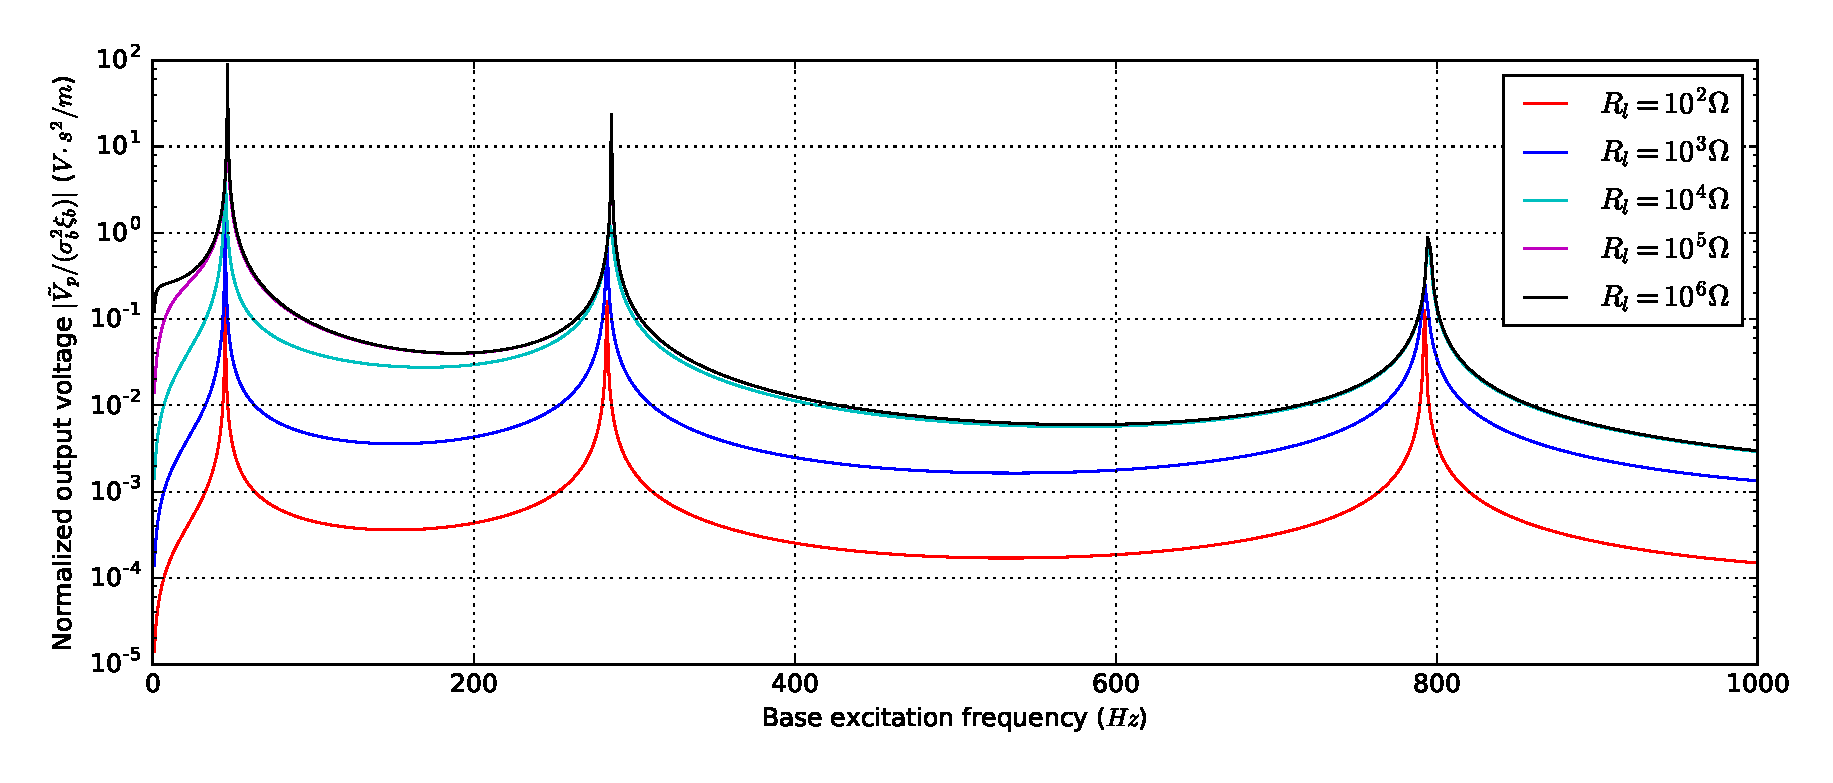
\includegraphics[width=\textwidth]{./img_eig_asy/fig_sol_analytic_perf_vs_fr}
    \caption{Validation calculation of the normalized output voltage versus base excitation frequency for a unimorph piezoelectric cantilever energy harvester based on the data from \cite{erturk2008distributed}.}
    \label{fig:fig_sol_analytic_perf_vs_fr}
\end{figure}

Secondly, according to equations (\ref{eq:eq_disp_func_general_coeffs}) and (\ref{eq:eq_disp_func_coeffs_exps}), the dimensionless displacement amplitude function $u(z)$ is totally determined by the three dimensionless parameters $\sigma$, $\beta$, and $\delta$ introduced before. Among the dimensionless parameters, $\sigma$ is the dimensionless base excitation frequency, $\beta$ is the dimensionless electrical resonant frequency, and $\delta$ is the dimensionless electromechanical coupling strength for the structure. As $\sigma$ and $\beta$ is determined by the base excitation and externally connected circuit respectively, only the parameter $\delta$ is fully determined by the structure itself. Hence we would like to investigate the influence of parameter $\delta$ upon the solution displacement function $u(z)$. By taking different values of $\delta$ , we calculate the displacement amplitude function $u(z)$ and plot the results in Figure~\ref{fig:fig_sol_analytic_disp_fun}.

\begin{figure}[!htbp]
    \centering
    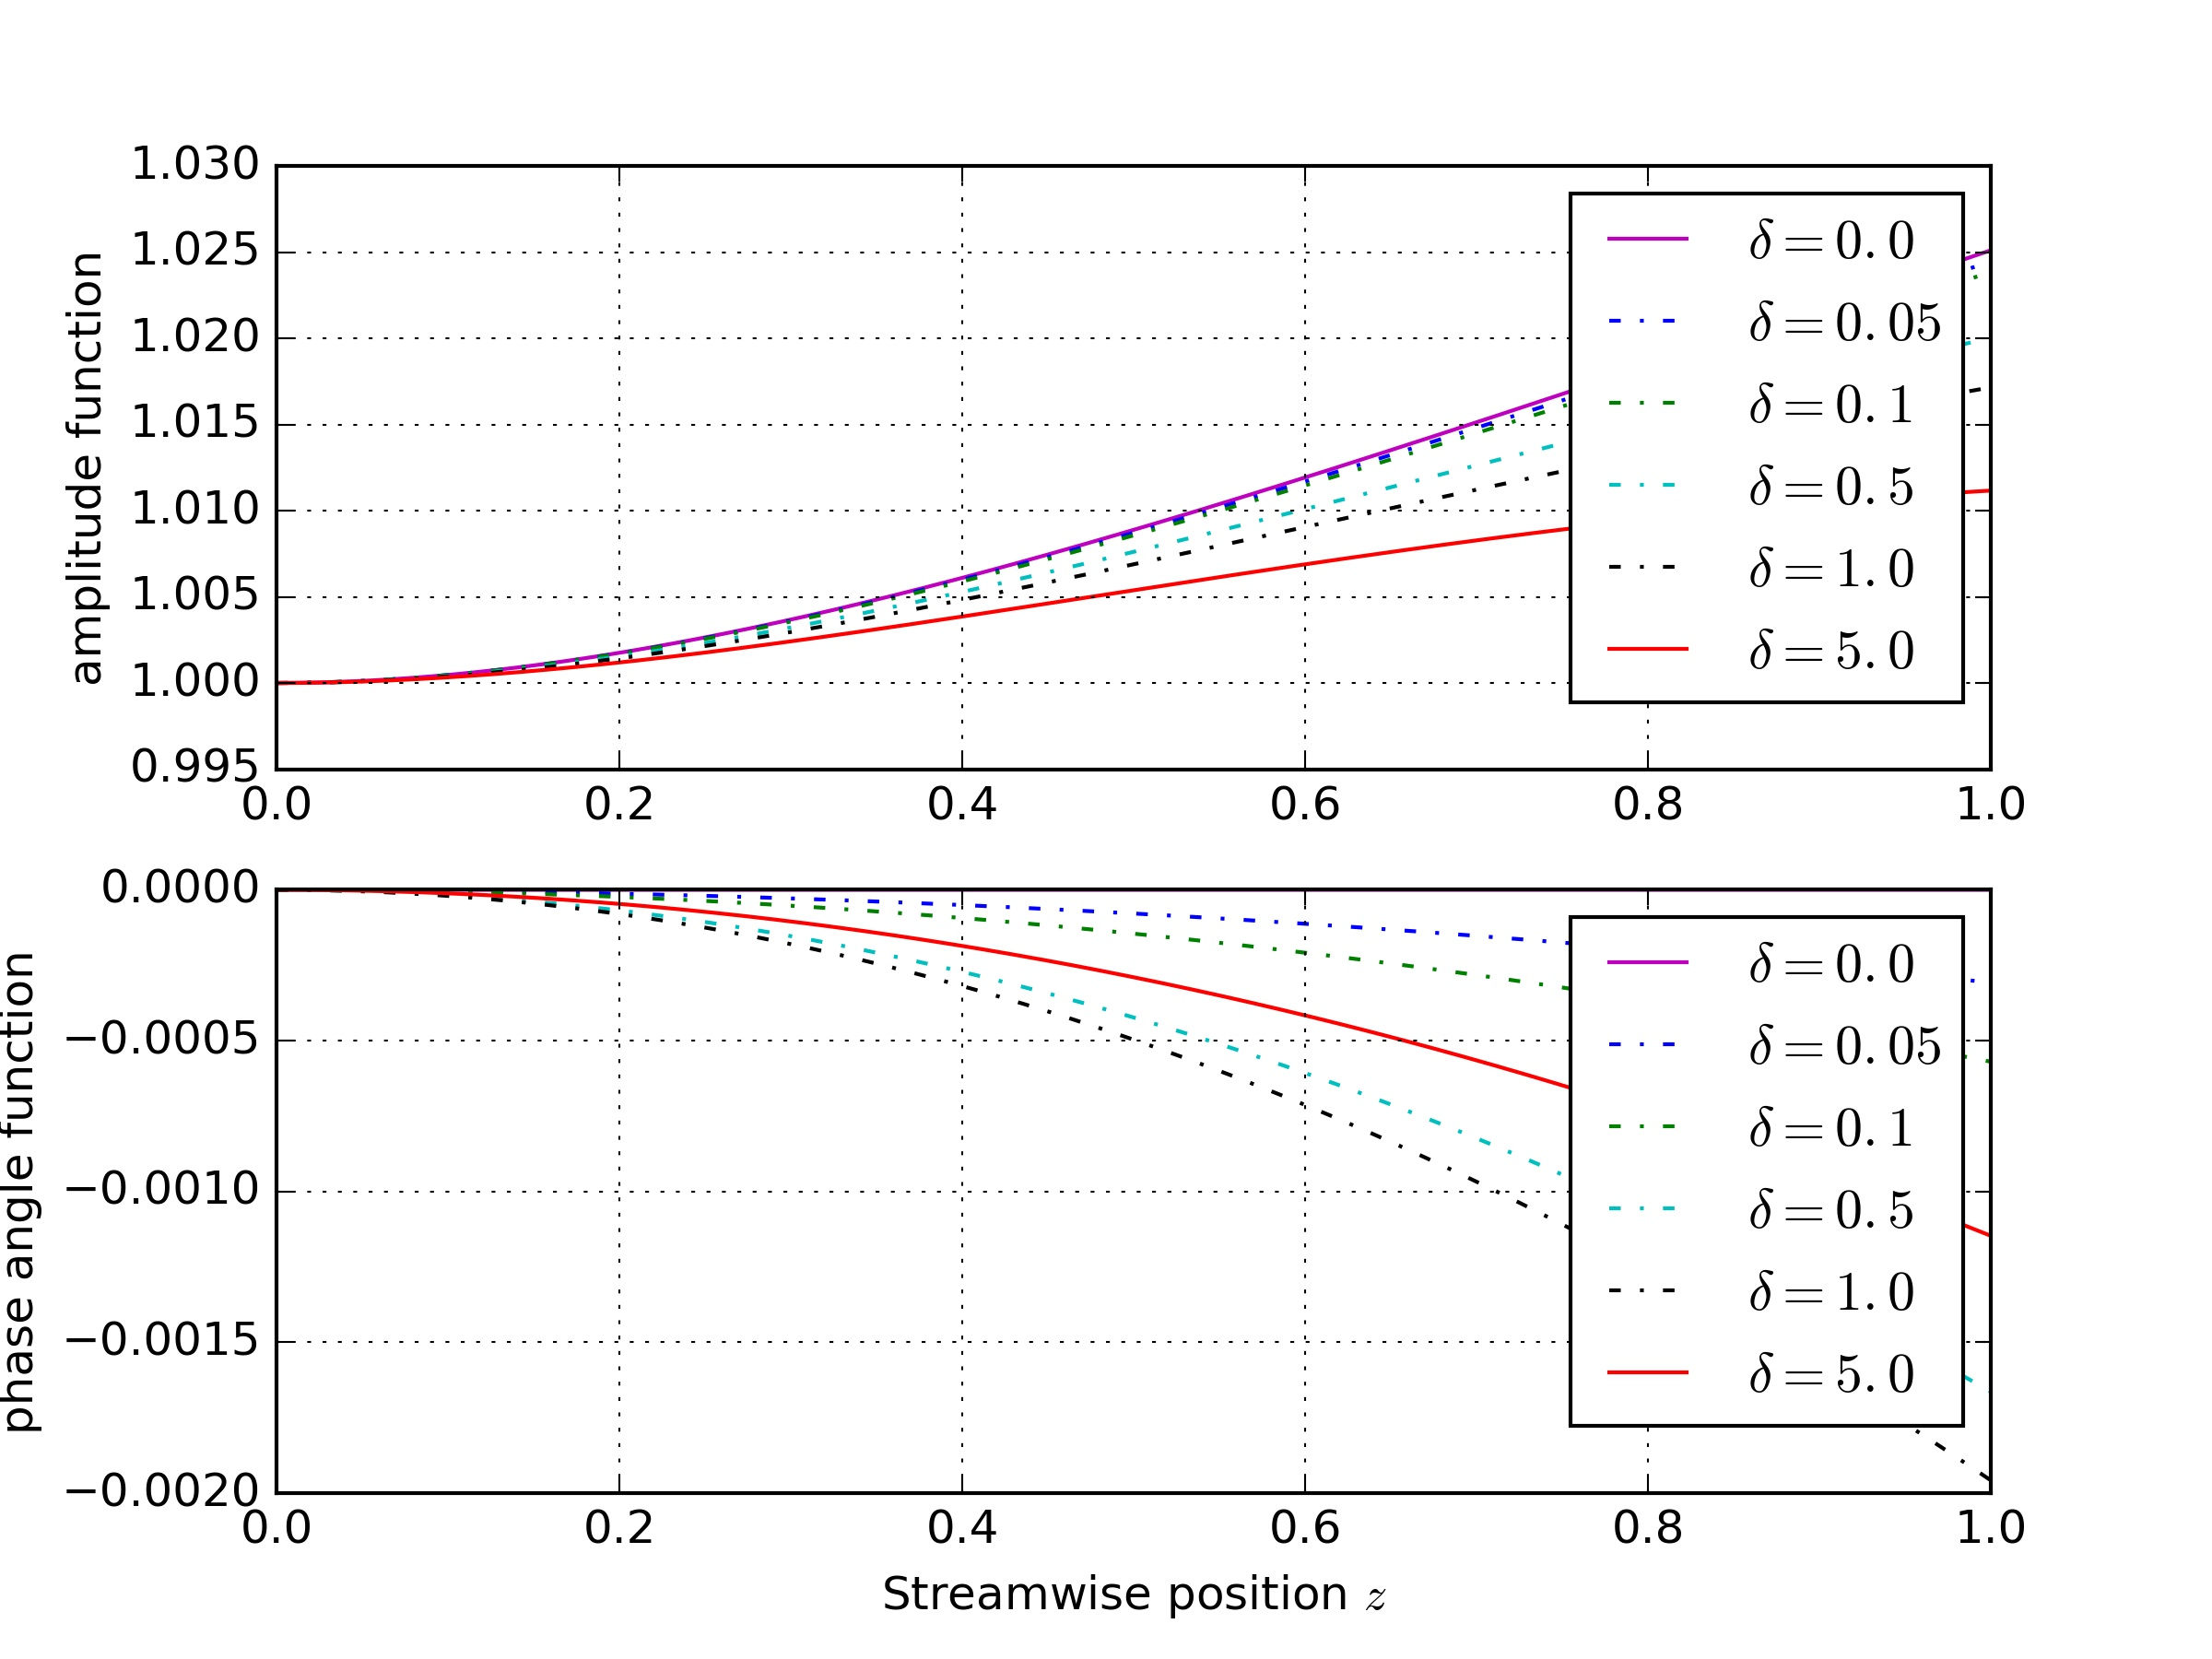
\includegraphics[width=\textwidth]{./img_eig_asy/fig_sol_analytic_disp_fun.jpg}
    \caption{Amplitude and phase of the displacement function $u(z)$ for difference values of $\delta$ }
    \label{fig:fig_sol_analytic_disp_fun}
\end{figure}





It is shown in Figure~\ref{fig:fig_sol_analytic_disp_fun}, the parameter $\delta$ changes the function $u(z)$ through the change of the third boundary condition (\textcolor{red}{to be inserted}). When $\delta$ is zero, i.e., no electromechanical coupling is present, the system degenerates to the classical elastic cantilever beam problem, whose solution is a real function. That is to say, the phase of $u(z)$ is a constant across the whole beam (in the range of $0 \leq z \leq 1$).
Analytical expressions for the coefficients are 
\begin{equation}
    \left\{\begin{aligned}
        A_{\varnothing} &= \frac{ 1 + \cos\sqrt{\sigma } \cosh\sqrt{\sigma } - \sin\sqrt{\sigma } \sinh\sqrt{\sigma} }{2 \left[ 1 + \cos\sqrt{\sigma } \cosh\sqrt{\sigma } \right]}, \\
        B_{\varnothing} &= \frac{ \cos\sqrt{\sigma } \sinh\sqrt{\sigma } + \sin\sqrt{\sigma } \cosh\sqrt{\sigma} }{2 \left[ 1 + \cos\sqrt{\sigma } \cosh\sqrt{\sigma } \right]}, \\
        C_{\varnothing} &= \frac{ 1 + \cos\sqrt{\sigma } \cosh\sqrt{\sigma } + \sin\sqrt{\sigma } \sinh\sqrt{\sigma} }{2 \left[ 1 + \cos\sqrt{\sigma } \cosh\sqrt{\sigma } \right]}, \\
        D_{\varnothing} &= \frac{ -\cos\sqrt{\sigma } \sinh\sqrt{\sigma } - \sin\sqrt{\sigma } \cosh\sqrt{\sigma} }{2 \left[ 1 + \cos\sqrt{\sigma } \cosh\sqrt{\sigma } \right]}.
    \end{aligned}\right.
    \label{eq:eq_disp_func_coeffs_exps_zero}
\end{equation}
and the resulting dimensionless displacement function $u_{\varnothing} (z)$ is represented as
\begin{equation}
    u_{\varnothing} (z) = A_{\varnothing} \cos{\sqrt{\sigma}z} + B_{\varnothing} \sin{\sqrt{\sigma}z} + C_{\varnothing} \cosh{\sqrt{\sigma}z} + D_{\varnothing} \sinh{\sqrt{\sigma}z} - 1.
\end{equation}
When the electromechanical coupling is extremely strong, and $\delta$ is extremely large and can be seen as $\infty$ in mathematical sense. In this situation, the solution $u_\infty (z)$ is again real without any phase difference in the $z$ direction. The coefficients can be analytically expressed as 
\begin{equation}
    \left\{\begin{aligned}
        A_\infty &= \frac{ \cos\sqrt{\sigma } \sinh\sqrt{\sigma } }{ \cos\sqrt{\sigma } \sinh\sqrt{\sigma } + \sin\sqrt{\sigma } \cosh\sqrt{\sigma } }, \\
        B_\infty &= \frac{ \sin\sqrt{\sigma } \sinh\sqrt{\sigma } }{ \cos\sqrt{\sigma } \sinh\sqrt{\sigma } + \sin\sqrt{\sigma } \cosh\sqrt{\sigma } }, \\
        C_\infty &= \frac{ \sin\sqrt{\sigma } \cosh\sqrt{\sigma } }{ \cos\sqrt{\sigma } \sinh\sqrt{\sigma } + \sin\sqrt{\sigma } \cosh\sqrt{\sigma } }, \\
        D_\infty &= \frac{ - \sin\sqrt{\sigma } \sinh\sqrt{\sigma } }{ \cos\sqrt{\sigma } \sinh\sqrt{\sigma } + \sin\sqrt{\sigma } \cosh\sqrt{\sigma } }.
    \end{aligned}\right.
    \label{eq:eq_disp_func_coeffs_exps_infty}
\end{equation}
and hence the dimensionless displacement function $u_{\infty} (z)$ is
\begin{equation}
    u_{\infty} (z) = A_{\infty} \cos{\sqrt{\sigma}z} + B_{\infty} \sin{\sqrt{\sigma}z} + C_{\infty} \cosh{\sqrt{\sigma}z} + D_{\infty} \sinh{\sqrt{\sigma}z} - 1.
\end{equation}
While a finite non-zero electromechanical coupling factor $\delta$ is present, which is expected in most applications, the resulting dimensionless displacement function $u(z)$ has varying magnitude and phase along the stream-wise direction or $z$ direction. Nevertheless, it is seen from the right panel of Figure~\ref{fig:fig_sol_analytic_disp_fun} that for different values of $\delta$, the phase change of $u(z)$ is very small in the $z$ direction, actually in the order $10^{-2}$. 


\begin{figure}[!htbp]
    \centering
    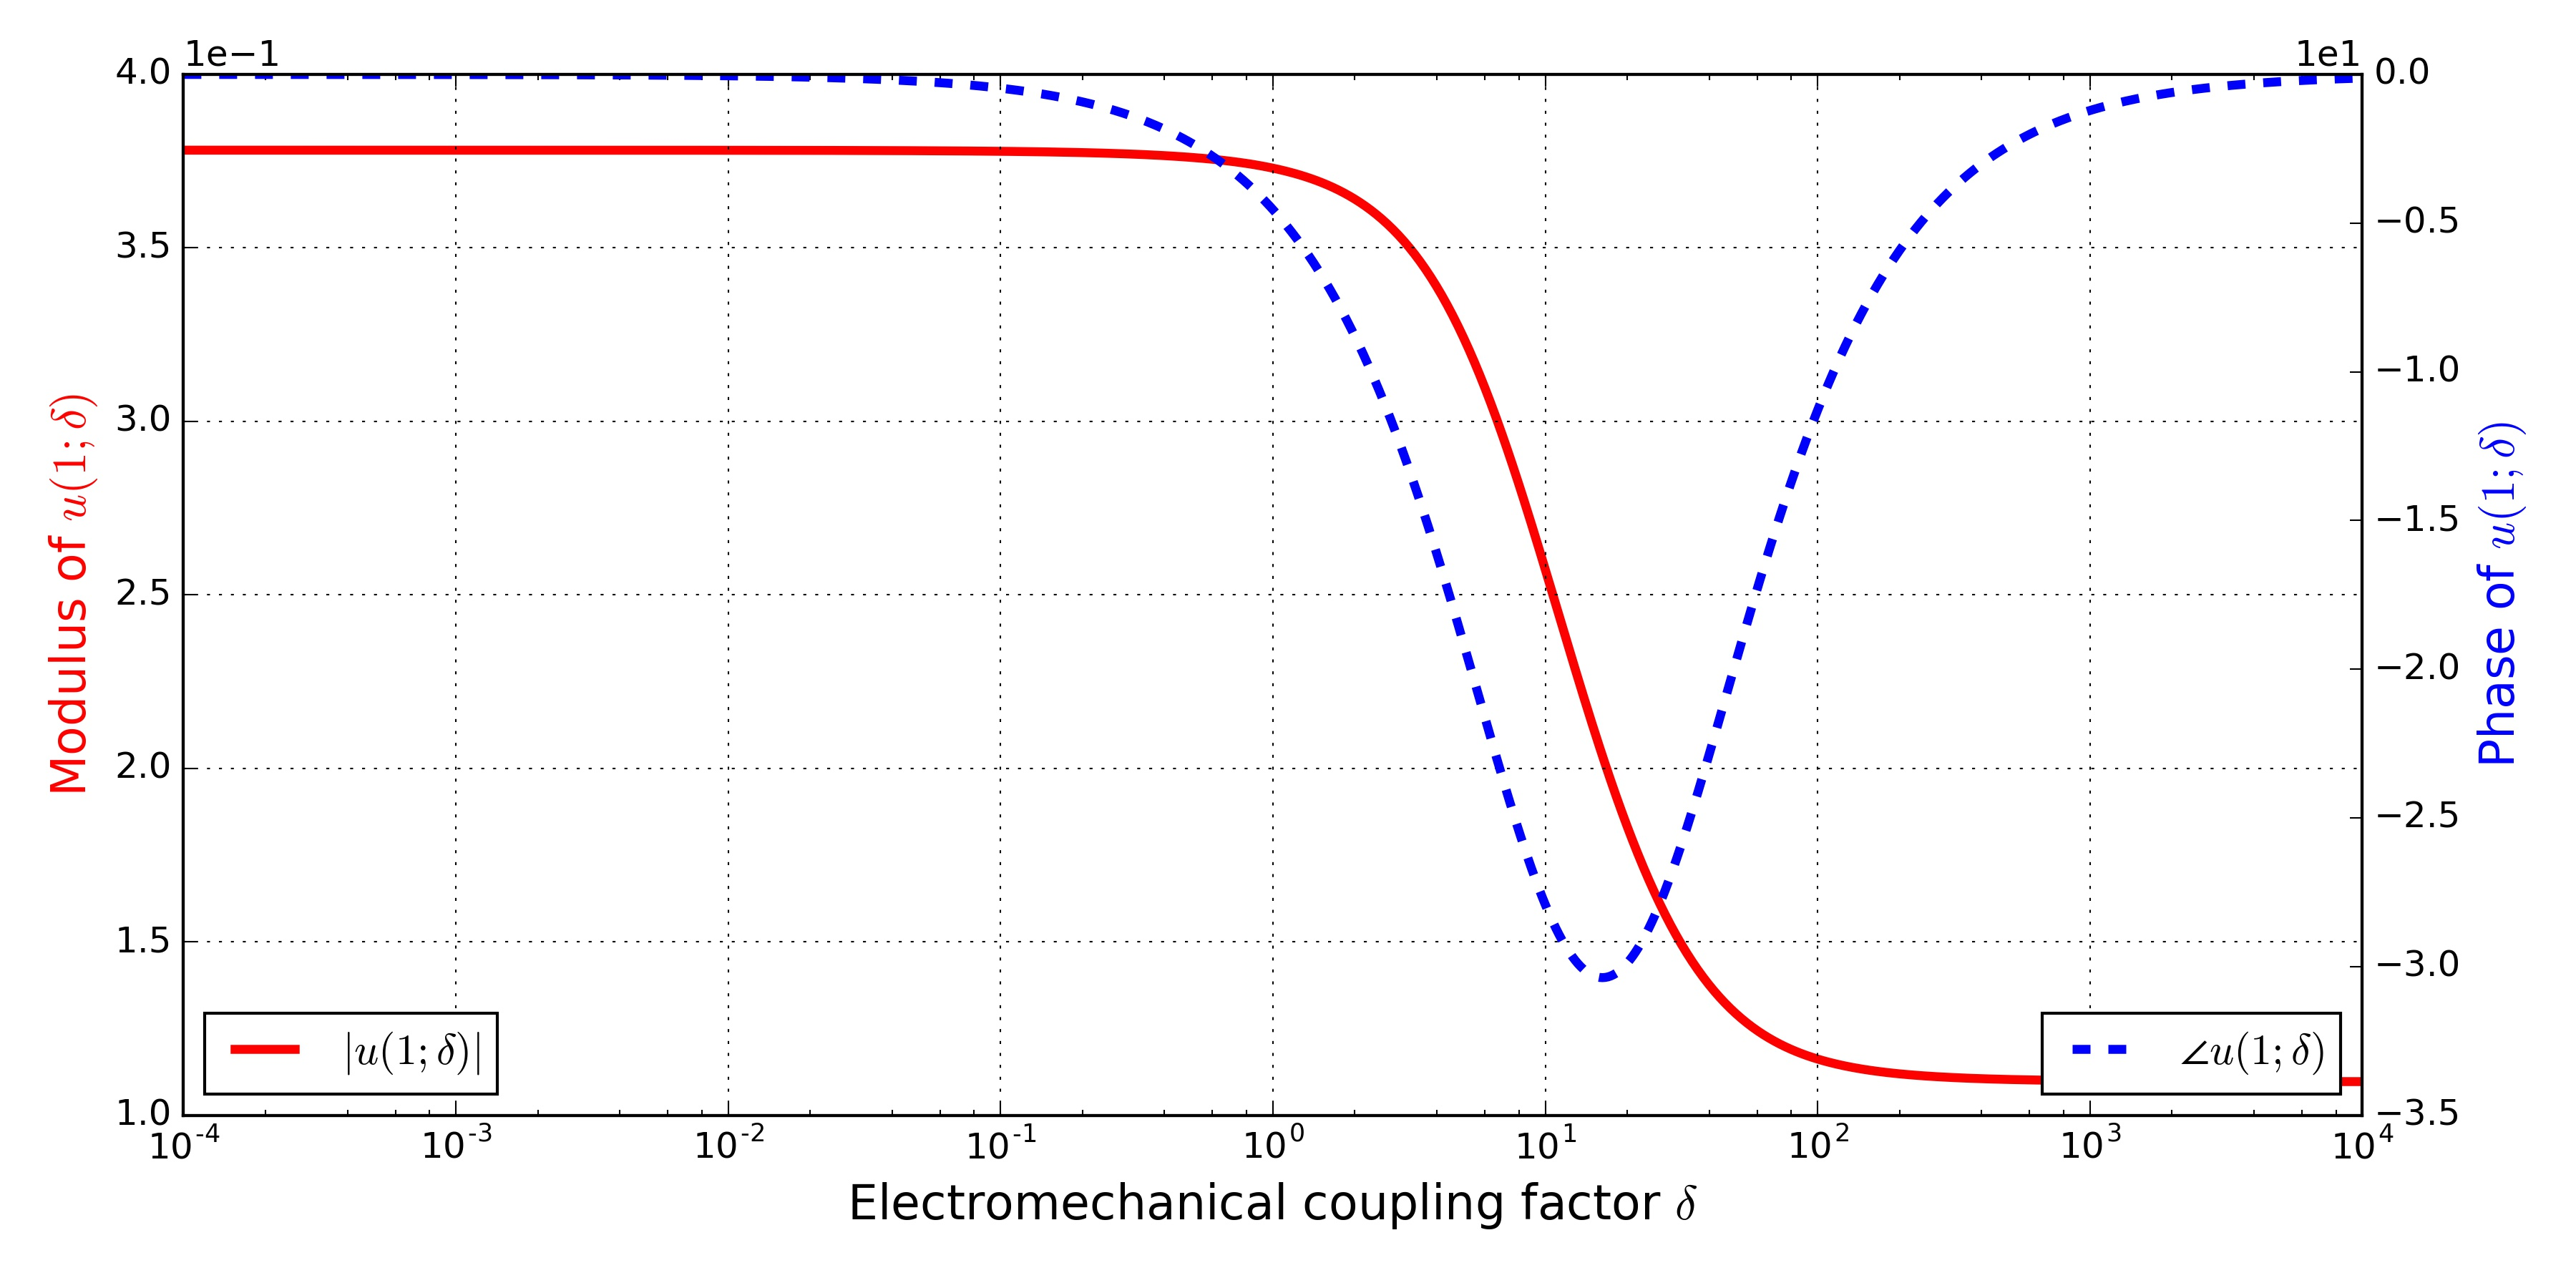
\includegraphics[width=0.8\textwidth]{./img_eig_asy/fig_sol_analytic_disp_end.jpg}
    \caption{Amplitude and phase of the displacement function $u(z)$ at the position $z=1$ versus electromechanical coupling factor $\delta$. }
    \label{fig:fig_sol_analytic_disp_end}
\end{figure}


To make it more clear, we plot the phase of $u(z)$ at $z=1$ versus different values of $\delta$ in Figure~\ref{fig:fig_sol_analytic_disp_end}. It is clear that with the increase of $\delta$, amplitude of the end displacement $(z=1)$ of the beam $|u(z)|$ decreases, while its phase reaches a minimum at around $\delta = 10$. This also explains the fact expressed in Figure~\ref{fig:fig_sol_analytic_disp_fun} that the amplitude of displacement function $u_\delta (z)$ with $0 < \delta < \infty$ is always between that of $u_\varnothing (z)$ and $u_\infty (z)$.


As for the output voltage $V_p(t)$, output current $I_p(t)$, and output power $P_p(t)$ for the classical piezoelectric cantilever energy harvester, their corresponding complex amplitudes $\tilde{V}_p$, $\tilde{I}_p$, and $\tilde{P}_p$ can be formulated as
\begin{equation}
    \left\{\begin{aligned}
        \tilde{V}_p &= -\frac{j \sigma \beta}{j \sigma \beta + 1} \frac{\eta_b}{l_p} \frac{e_p}{C_p} u^\prime(1), \\
        &= -\frac{j \sigma \beta}{j \sigma \beta + 1} \frac{\eta_b}{l_p} \frac{e_p}{C_p} \sigma^{1/2} \left( - A_\delta \sin{\sqrt{\sigma}} + B_\delta \cos{\sqrt{\sigma}} + C_\delta \sinh{\sqrt{\sigma}} + D_\delta \cosh{\sqrt{\sigma}} \right) \\
        &= - \frac{j \sigma \beta}{j \sigma \beta + 1} \frac{\eta_b}{l_p} \frac{e_p}{C_p}  \frac{ \sqrt{\sigma} \left( \sinh\sqrt{\sigma} - \sin\sqrt{\sigma} \right) }{ 1 + \cos\sqrt{\sigma } \cosh\sqrt{\sigma } + \frac{j \beta \sqrt{\sigma}}{ 1+ j \beta \sigma } \delta \left( \cos\sqrt{\sigma } \sinh\sqrt{\sigma } + \sin\sqrt{\sigma } \cosh\sqrt{\sigma } \right) }\\
        &= - \frac{j \sigma \beta}{j \sigma \beta + 1} \left(\frac{\eta_b}{l_p}\right) \left(\frac{e_p}{C_p}\right) \chi_p , \\
        \tilde{I}_p &=  \tilde{V}_p / R_l = - \frac{ j \sigma \beta } {j \sigma \beta + 1} \left( \frac{\eta_b}{l_p} \right) \left( \frac{e_p}{C_p R_l} \right) \chi_p , \\
        \tilde{P}_p &=  \tilde{V}_p^2 / R_l = \left(\frac{\eta_b}{l_p}\right)^2 \left(\frac{e_p}{C_p}\right) \left( \frac{e_p}{C_p R_l} \right) \left( \frac{ j \sigma \beta}{ j \sigma \beta + 1 } \right)^2 \chi_p^2∫,
    \end{aligned}\right.
    \label{eq:eq_peh_perfs_compact_form}
\end{equation}
in which we have used the notations that 
\begin{equation}
    \chi_p = u_1^\prime(1) = \frac{ \sqrt{\sigma} \left( \sinh\sqrt{\sigma} - \sin\sqrt{\sigma} \right) }{ 1 + \cos\sqrt{\sigma } \cosh\sqrt{\sigma } + \frac{j \beta \sqrt{\sigma}}{ 1+ j \beta \sigma } \delta \left( \cos\sqrt{\sigma } \sinh\sqrt{\sigma } + \sin\sqrt{\sigma } \cosh\sqrt{\sigma } \right) }.
    \label{eq:eq_peh_perfs_compact_form_end_ders}
\end{equation}
Clearly, The three output measures $\tilde{V}_p$, $\tilde{I}_p$, and $\tilde{P}_p$ are heavily dependent on another dimensionless parameter $r_d = \eta_b/l_p$. Formally, both $\tilde{V}_p$ and $\tilde{I}_p$ depend linearly upon $r_d$, while $\tilde{P}_p$ shows a quadratic dependence on $r_d$. The only dependence upon $\delta$ is introduced in $\chi_p$. However, it should be noted that the parameter $\delta$ relies on $e_p$, $l_p$, $C_p$, and $B_p$, while the three measures $\tilde{V}_p$, $\tilde{I}_p$, and $\tilde{P}_p$ are dimensional values and depend on $e_p$, $\sigma_b$, and $R_l$. As a result, the change of parameter $\delta$ results in the change of reference voltage $e_p / C_p$, reference current $e_p / (C_p R_l)$, and reference power $(e_p / C_p)[e_p / (C_p R_l)]$, and therefore the corresponding values of $\tilde{V}_p$, $\tilde{I}_p$, and $\tilde{P}_p$. Hence, we may establish a bijective relation between $\delta$ and $e_p$, and relate the change of $\delta$ to that of $e_p$. In this way, we calculate the output measures at different values of $\delta$ and plot their amplitudes in Figure~\ref{fig:fig_sol_analytic_perf_fun}. 
\begin{figure}[!htbp]
    \centering
    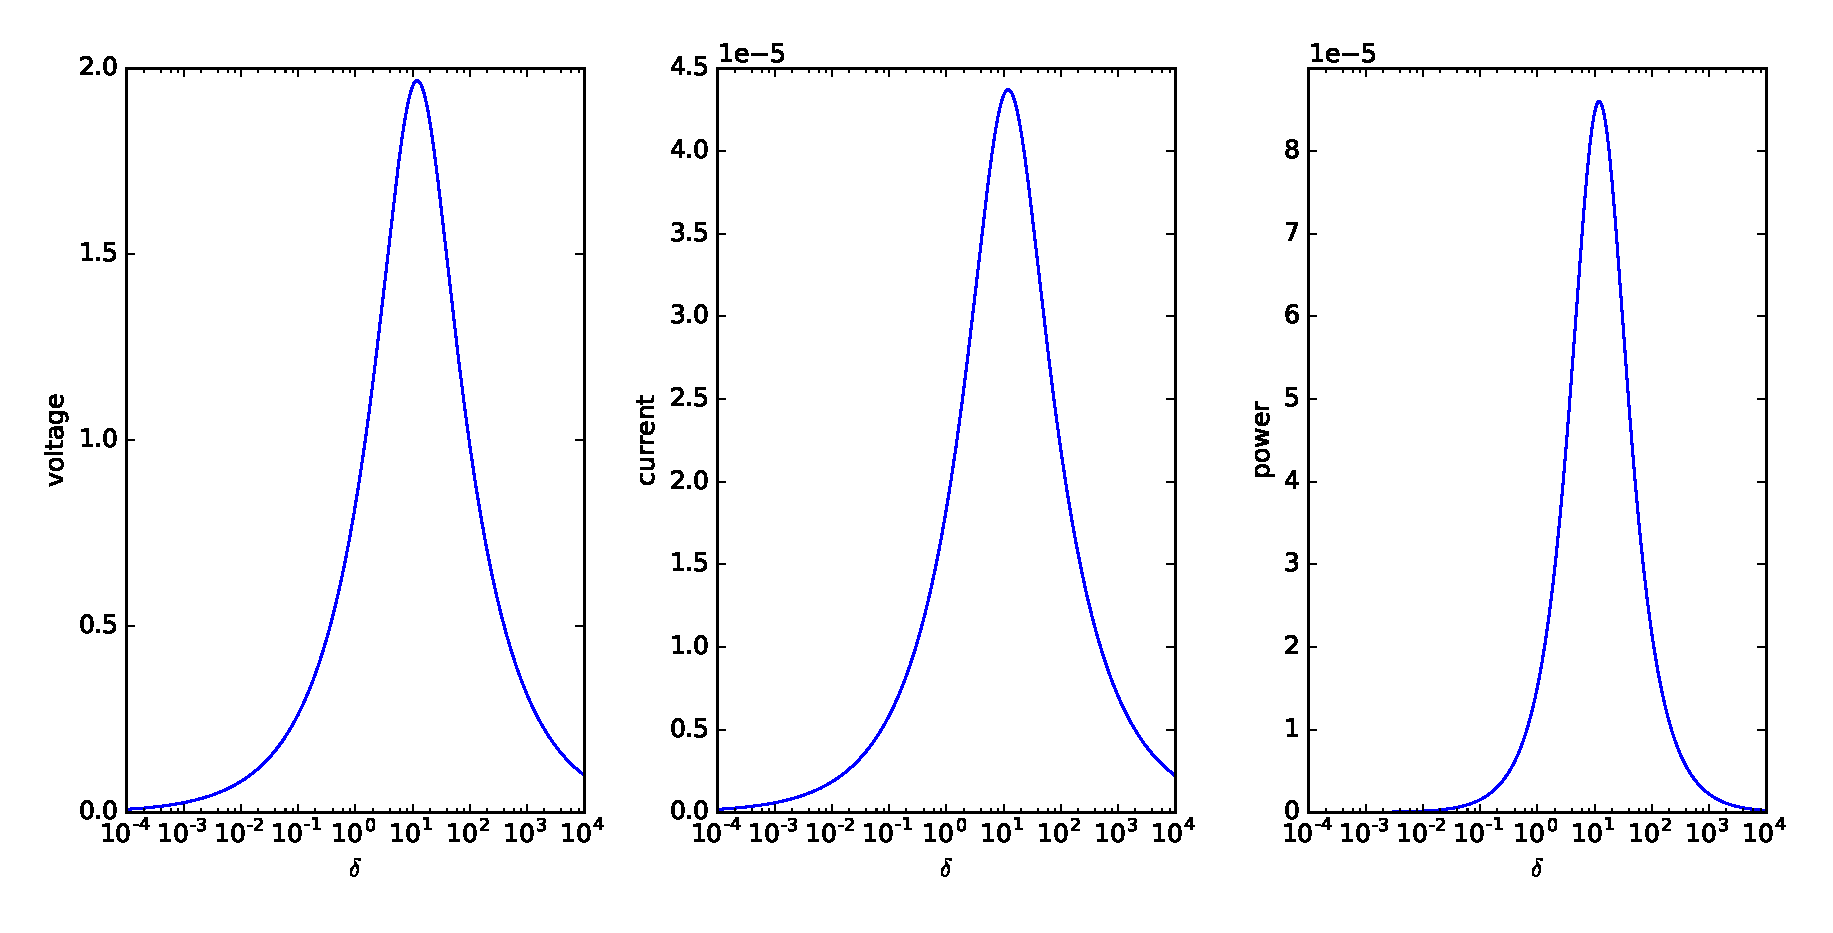
\includegraphics[width=\textwidth]{./img_eig_asy/fig_sol_analytic_perf_fun}
    \caption{Voltage, current and power output for the piezoelectric cantilever energy harvester}
    \label{fig:fig_sol_analytic_perf_fun}
\end{figure}
% For a typical piezoelectric cantilever energy harvester in the literature \cite{erturk2008distributed,erturk2009experimentally}, this parameter $\delta$ is rather small


It is seen from Figure~\ref{fig:fig_sol_analytic_perf_fun} that all the three measures show a maximum peak with the increase of $\delta$ at the approximate value of $\delta = 10$. When $\delta$ is small, or equivalently, $e_p$ is small, amplitude of the three output measures $\tilde{V}_p$, $\tilde{I}_p$, and $\tilde{P}_p$ increase with the increase of $\delta$. Then after the critical value of $\delta$, a further increase of $\delta$ causes the decrease of output measures. Thus we come to a small conclusion that to obtain an optimal output performance, the electromechanical coupling factor $\delta$ should be set to an appropriate value. However, a direct calculation using the parameters introduced in the literature \cite{erturk2008distributed,erturk2009experimentally} shows that the parameter $\delta$ is rather small for a typical piezoelectric cantilever energy harvester. For example, for a piezoelectric voltage constant $e_{31} = -5.35\ C / m^2$, the value of $e_p$ is $-5.35 \times 10^{-5}\ C$, and the final value of $\delta$ is $0.028$. According to the properties of commonly used piezoelectric materials, the parameter $e_{31}$ is always in the range of several or several tens $C / m^2$ \textcolor{red}{reference to be inserted}. That is to say, the final value of $\delta$ can be seen always in the order of $10^{-2}$, which is a rather small value according to the diagram. Hence we could present an asymptotic analysis of the performance of the classical piezoelectric energy harvester. This is the subject of the following section.


\section{Asymptotic analysis of the problem}

Considering that the parameter $\delta$ is small, we expand the theoretical solution to the problem in terms of the small parameter $\delta$ using the following regular expansion:
\begin{equation}
    \left\{\begin{aligned}
        A_\delta &= A_0 + \delta A_1 + \delta^2 A_2 + \cdots, \\
        B_\delta &= B_0 + \delta B_1 + \delta^2 B_2 + \cdots, \\
        C_\delta &= C_0 + \delta C_1 + \delta^2 C_2 + \cdots, \\
        D_\delta &= D_0 + \delta D_1 + \delta^2 D_2 + \cdots. 
    \end{aligned}\right.
\end{equation}
As a result, we obtain the following successive expansion problem:

\noindent
$O(\delta^0)$:
\begin{equation}
    \left\{\begin{aligned}
        A_0 + C_0 &= 1, \\
        B_0 + D_0 &= 0, \\
        - A_0 \cos{\sqrt{\sigma}} - B_0 \sin{\sqrt{\sigma}} + C_0 \cosh{\sqrt{\sigma}} + D_0 \sinh{\sqrt{\sigma}} &= 0, \\
        A_0 \sin{\sqrt{\sigma}} - B_0 \cos{\sqrt{\sigma}} + C_0 \sinh{\sqrt{\sigma}} + D_0 \cosh{\sqrt{\sigma}} &= 0.
    \end{aligned}\right.
\end{equation}
The solution is
\begin{equation}
    \left\{\begin{aligned}
        A_0 &= \frac{1 + \cos\sqrt{\sigma} \cosh\sqrt{\sigma} - \sin\sqrt{\sigma} \sinh\sqrt{\sigma} }{2 + 2 \cos\sqrt{\sigma} \cosh\sqrt{\sigma} }, \\
        B_0 &= \frac{\cosh\sqrt{\sigma} \sin\sqrt{\sigma} + \cos\sqrt{\sigma} \sinh\sqrt{\sigma} }{2 + 2 \cos\sqrt{\sigma} \cosh\sqrt{\sigma} }, \\
        C_0 &= \frac{1 + \cos\sqrt{\sigma} \cosh\sqrt{\sigma} + \sin\sqrt{\sigma} \sinh\sqrt{\sigma} }{2 + 2 \cos\sqrt{\sigma} \cosh\sqrt{\sigma} }, \\
        D_0 &= -\frac{\cosh\sqrt{\sigma} \sin\sqrt{\sigma} + \cos\sqrt{\sigma} \sinh\sqrt{\sigma} }{2 + 2 \cos\sqrt{\sigma} \cosh\sqrt{\sigma} }.
    \end{aligned}\right.
\end{equation}
Hence we have
\begin{equation}
    - A_0 \sin{\sqrt{\sigma}} + B_0 \cos{\sqrt{\sigma}} + C_0 \sinh{\sqrt{\sigma}} + D_0 \cosh{\sqrt{\sigma}} = \frac{\sinh\sqrt{\sigma }-\sin\sqrt{\sigma }}{\cos\sqrt{\sigma } \cosh\sqrt{\sigma }+1}
\end{equation}

\noindent
$O(\delta^1)$:
\begin{equation}
    \left\{\begin{aligned}
        A_1 + C_1 &= 0, \\
        B_1 + D_1 &= 0, \\
        \left( - A_1 \cos{\sqrt{\sigma}} - B_1 \sin{\sqrt{\sigma}} + C_1 \cosh{\sqrt{\sigma}} + D_1 \sinh{\sqrt{\sigma}} \right) &+ \\
        \frac{j \beta \sqrt{\sigma}}{ j\sigma \beta + 1 } \left( - A_0 \sin{\sqrt{\sigma}} + B_0 \cos{\sqrt{\sigma}} + C_0 \sinh{\sqrt{\sigma}} + D_0 \cosh{\sqrt{\sigma}} \right) &= 0, \\
        A_1 \sin{\sqrt{\sigma}} - B_1 \cos{\sqrt{\sigma}} + C_1 \sinh{\sqrt{\sigma}} + D_1 \cosh{\sqrt{\sigma}} &= 0.
    \end{aligned}\right.
\end{equation}
The solution is
\begin{equation}
    \left\{\begin{aligned}
        A_1 &= \frac{j \beta  \sqrt{\sigma }}{1+j \beta  \sigma } \left( \frac{\sinh\sqrt{\sigma }-\sin\sqrt{\sigma }}{\cos\sqrt{\sigma } \cosh\sqrt{\sigma }+1} \right) \left(\frac{\cos\sqrt{\sigma }+\cosh\sqrt{\sigma }}{2 \cos\sqrt{\sigma }\cosh\sqrt{\sigma }+2} \right) \\
        B_1 &= \frac{j \beta  \sqrt{\sigma }}{1+j \beta  \sigma } \left( \frac{\sinh\sqrt{\sigma }-\sin\sqrt{\sigma }}{\cos\sqrt{\sigma } \cosh\sqrt{\sigma }+1} \right) \left( \frac{-\sinh\sqrt{\sigma }+\sin\sqrt{\sigma }}{2 \cos\sqrt{\sigma }\cosh\sqrt{\sigma }+2} \right)\\
        C_1 &= \frac{j \beta  \sqrt{\sigma }}{1+j \beta  \sigma } \left( \frac{\sinh\sqrt{\sigma }-\sin\sqrt{\sigma }}{\cos\sqrt{\sigma } \cosh\sqrt{\sigma }+1} \right) \left( -\frac{\cos\sqrt{\sigma }+\cosh\sqrt{\sigma }}{2 \cos\sqrt{\sigma } \cosh\sqrt{\sigma }+2} \right)\\
        D_1 &= \frac{j \beta  \sqrt{\sigma }}{1+j \beta  \sigma } \left( \frac{\sinh\sqrt{\sigma }-\sin\sqrt{\sigma }}{\cos\sqrt{\sigma } \cosh\sqrt{\sigma }+1} \right) \left( \frac{-\sin\sqrt{\sigma }+\sinh\sqrt{\sigma }}{2 \cos\sqrt{\sigma }\cosh\sqrt{\sigma }+2} \right)
    \end{aligned}\right.
\end{equation}
Then we have
\begin{equation}
    \begin{aligned}
        - A_1 \sin{\sqrt{\sigma}} + B_1 \cos{\sqrt{\sigma}} + C_1 \sinh{\sqrt{\sigma}} + D_1 \cosh{\sqrt{\sigma}} \\
        = \frac{j \beta  \sqrt{\sigma }}{1+j \beta  \sigma } \left(\frac{\sin\sqrt{\sigma } -\sinh\sqrt{\sigma }}{\cos\sqrt{\sigma } \cosh\sqrt{\sigma }+1} \right)  \left( \frac{\cos\sqrt{\sigma } \sinh\sqrt{\sigma }+\sin\sqrt{\sigma } \cosh\sqrt{\sigma }}{\cos\sqrt{\sigma } \cosh\sqrt{\sigma }+1} \right)
    \end{aligned}
\end{equation}

\noindent
$O(\delta^2)$:
\begin{equation}
    \left\{\begin{aligned}
        A_2 + C_2 &= 0, \\
        B_2 + D_2 &= 0, \\
        \left( - A_2 \cos{\sqrt{\sigma}} - B_2 \sin{\sqrt{\sigma}} + C_2 \cosh{\sqrt{\sigma}} + D_2 \sinh{\sqrt{\sigma}} \right) &+ \\
        \frac{j \beta \sqrt{\sigma}}{ j\sigma \beta + 1 } \left( - A_1 \sin{\sqrt{\sigma}} + B_1 \cos{\sqrt{\sigma}} + C_1 \sinh{\sqrt{\sigma}} + D_1 \cosh{\sqrt{\sigma}} \right) &= 0, \\
        A_2 \sin{\sqrt{\sigma}} - B_2 \cos{\sqrt{\sigma}} + C_2 \sinh{\sqrt{\sigma}} + D_2 \cosh{\sqrt{\sigma}} &= 0.
    \end{aligned}\right.
\end{equation}
The solution is
\scriptsize
\begin{equation}
    \left\{\begin{aligned}
        A_2 &= \left( \frac{j \beta \sqrt{\sigma }}{1+j \beta \sigma } \right)^2 \left(\frac{ \sinh\sqrt{\sigma } - \sin\sqrt{\sigma }}{\cos\sqrt{\sigma } \cosh\sqrt{\sigma }+1} \right) \left( \frac{\cos\sqrt{\sigma } \sinh\sqrt{\sigma }+\sin\sqrt{\sigma } \cosh\sqrt{\sigma }}{\cos\sqrt{\sigma } \cosh\sqrt{\sigma }+1} \right) \left(\frac{\cos\sqrt{\sigma }+\cosh\sqrt{\sigma }}{2 \cos\sqrt{\sigma }\cosh\sqrt{\sigma }+2} \right) \\
        B_2 &= \left( \frac{j \beta \sqrt{\sigma }}{1+j \beta \sigma } \right)^2 \left(\frac{\sinh\sqrt{\sigma } - \sin\sqrt{\sigma }}{\cos\sqrt{\sigma } \cosh\sqrt{\sigma }+1} \right) \left( \frac{\cos\sqrt{\sigma } \sinh\sqrt{\sigma }+\sin\sqrt{\sigma } \cosh\sqrt{\sigma }}{\cos\sqrt{\sigma } \cosh\sqrt{\sigma }+1} \right) \left( \frac{-\sinh\sqrt{\sigma }+\sin\sqrt{\sigma }}{2 \cos\sqrt{\sigma }\cosh\sqrt{\sigma }+2} \right)\\
        C_2 &= \left( \frac{j \beta \sqrt{\sigma }}{1+j \beta \sigma } \right)^2 \left(\frac{\sinh\sqrt{\sigma } - \sin\sqrt{\sigma }}{\cos\sqrt{\sigma } \cosh\sqrt{\sigma }+1} \right) \left( \frac{\cos\sqrt{\sigma } \sinh\sqrt{\sigma }+\sin\sqrt{\sigma } \cosh\sqrt{\sigma }}{\cos\sqrt{\sigma } \cosh\sqrt{\sigma }+1} \right) \left( -\frac{\cos\sqrt{\sigma }+\cosh\sqrt{\sigma }}{2 \cos\sqrt{\sigma } \cosh\sqrt{\sigma }+2} \right)\\
        D_2 &= \left( \frac{j \beta \sqrt{\sigma }}{1+j \beta \sigma } \right)^2 \left(\frac{\sinh\sqrt{\sigma } - \sin\sqrt{\sigma }}{\cos\sqrt{\sigma } \cosh\sqrt{\sigma }+1} \right) \left( \frac{\cos\sqrt{\sigma } \sinh\sqrt{\sigma }+\sin\sqrt{\sigma } \cosh\sqrt{\sigma }}{\cos\sqrt{\sigma } \cosh\sqrt{\sigma }+1} \right) \left( \frac{-\sin\sqrt{\sigma }+\sinh\sqrt{\sigma }}{2 \cos\sqrt{\sigma }\cosh\sqrt{\sigma }+2} \right)
    \end{aligned}\right.
\end{equation}
\normalsize

Indeed, we can continue to obtain the coefficients for higher order ($\geq 2$) expansions, as shown in the appendices (\textcolor{red}{To add some comments}) using successive iteration method. Nevertheless, it suffices here to consider up to the second order expansion $u^{(0)} (z)$, $u^{(1)} (z)$, and $u^{(2)} (z)$, respectively:
\begin{equation}
    \left\{\begin{aligned}
        u^{(0)} (z) &= u_0 (z), \\
        u^{(1)} (z) &= u_0 (z) + \delta u_1(z), \\
        u^{(2)} (z) &= u_0 (z) + \delta u_1(z) + \delta^2 u_2 (z),
    \end{aligned}\right.
\end{equation}
where the terms $u_0 (z)$, $u_1(z)$, and $u_2 (z)$ are defined as
\begin{equation}
    \left\{\begin{aligned}
        u_0 (z) &= A_0 \cos{\sqrt{\sigma}z} + B_0 \sin{\sqrt{\sigma}z} + C_0 \cosh{\sqrt{\sigma}z} + D_0 \sinh{\sqrt{\sigma}z} - 1, \\
        u_1 (z) &= A_1 \cos{\sqrt{\sigma}z} + B_1 \sin{\sqrt{\sigma}z} + C_1 \cosh{\sqrt{\sigma}z} + D_1 \sinh{\sqrt{\sigma}z}, \\
        u_2 (z) &= A_2 \cos{\sqrt{\sigma}z} + B_2 \sin{\sqrt{\sigma}z} + C_2 \cosh{\sqrt{\sigma}z} + D_2 \sinh{\sqrt{\sigma}z}.
    \end{aligned}\right.
\end{equation}


For different values of $\delta$ and $\sigma$ (Here in this simulation, the value of $\sigma$ is changed through the variance of base excitation frequency $f_b$), the asymptotic approximations of the dimensionless relative beam displacement function $u(z;\delta)$ up to the second order $u^{(0)}(z)$, $u^{(1)}(z)$, and $u^{(2)}(z)$ are calculated and compared to the closed solution $u(z;\delta)$ itself. The results are shown in Figure~\ref{fig:fig_sol_analytic_disp_cmp_fr001}, \ref{fig:fig_sol_analytic_disp_cmp_fr020}, \ref{fig:fig_sol_analytic_disp_cmp_fr040}, \ref{fig:fig_sol_analytic_disp_cmp_fr045}, \ref{fig:fig_sol_analytic_disp_cmp_fr060}, \ref{fig:fig_sol_analytic_disp_cmp_fr080}, \ref{fig:fig_sol_analytic_disp_cmp_fr100}. 


\begin{figure}[!htbp]
    \centering
    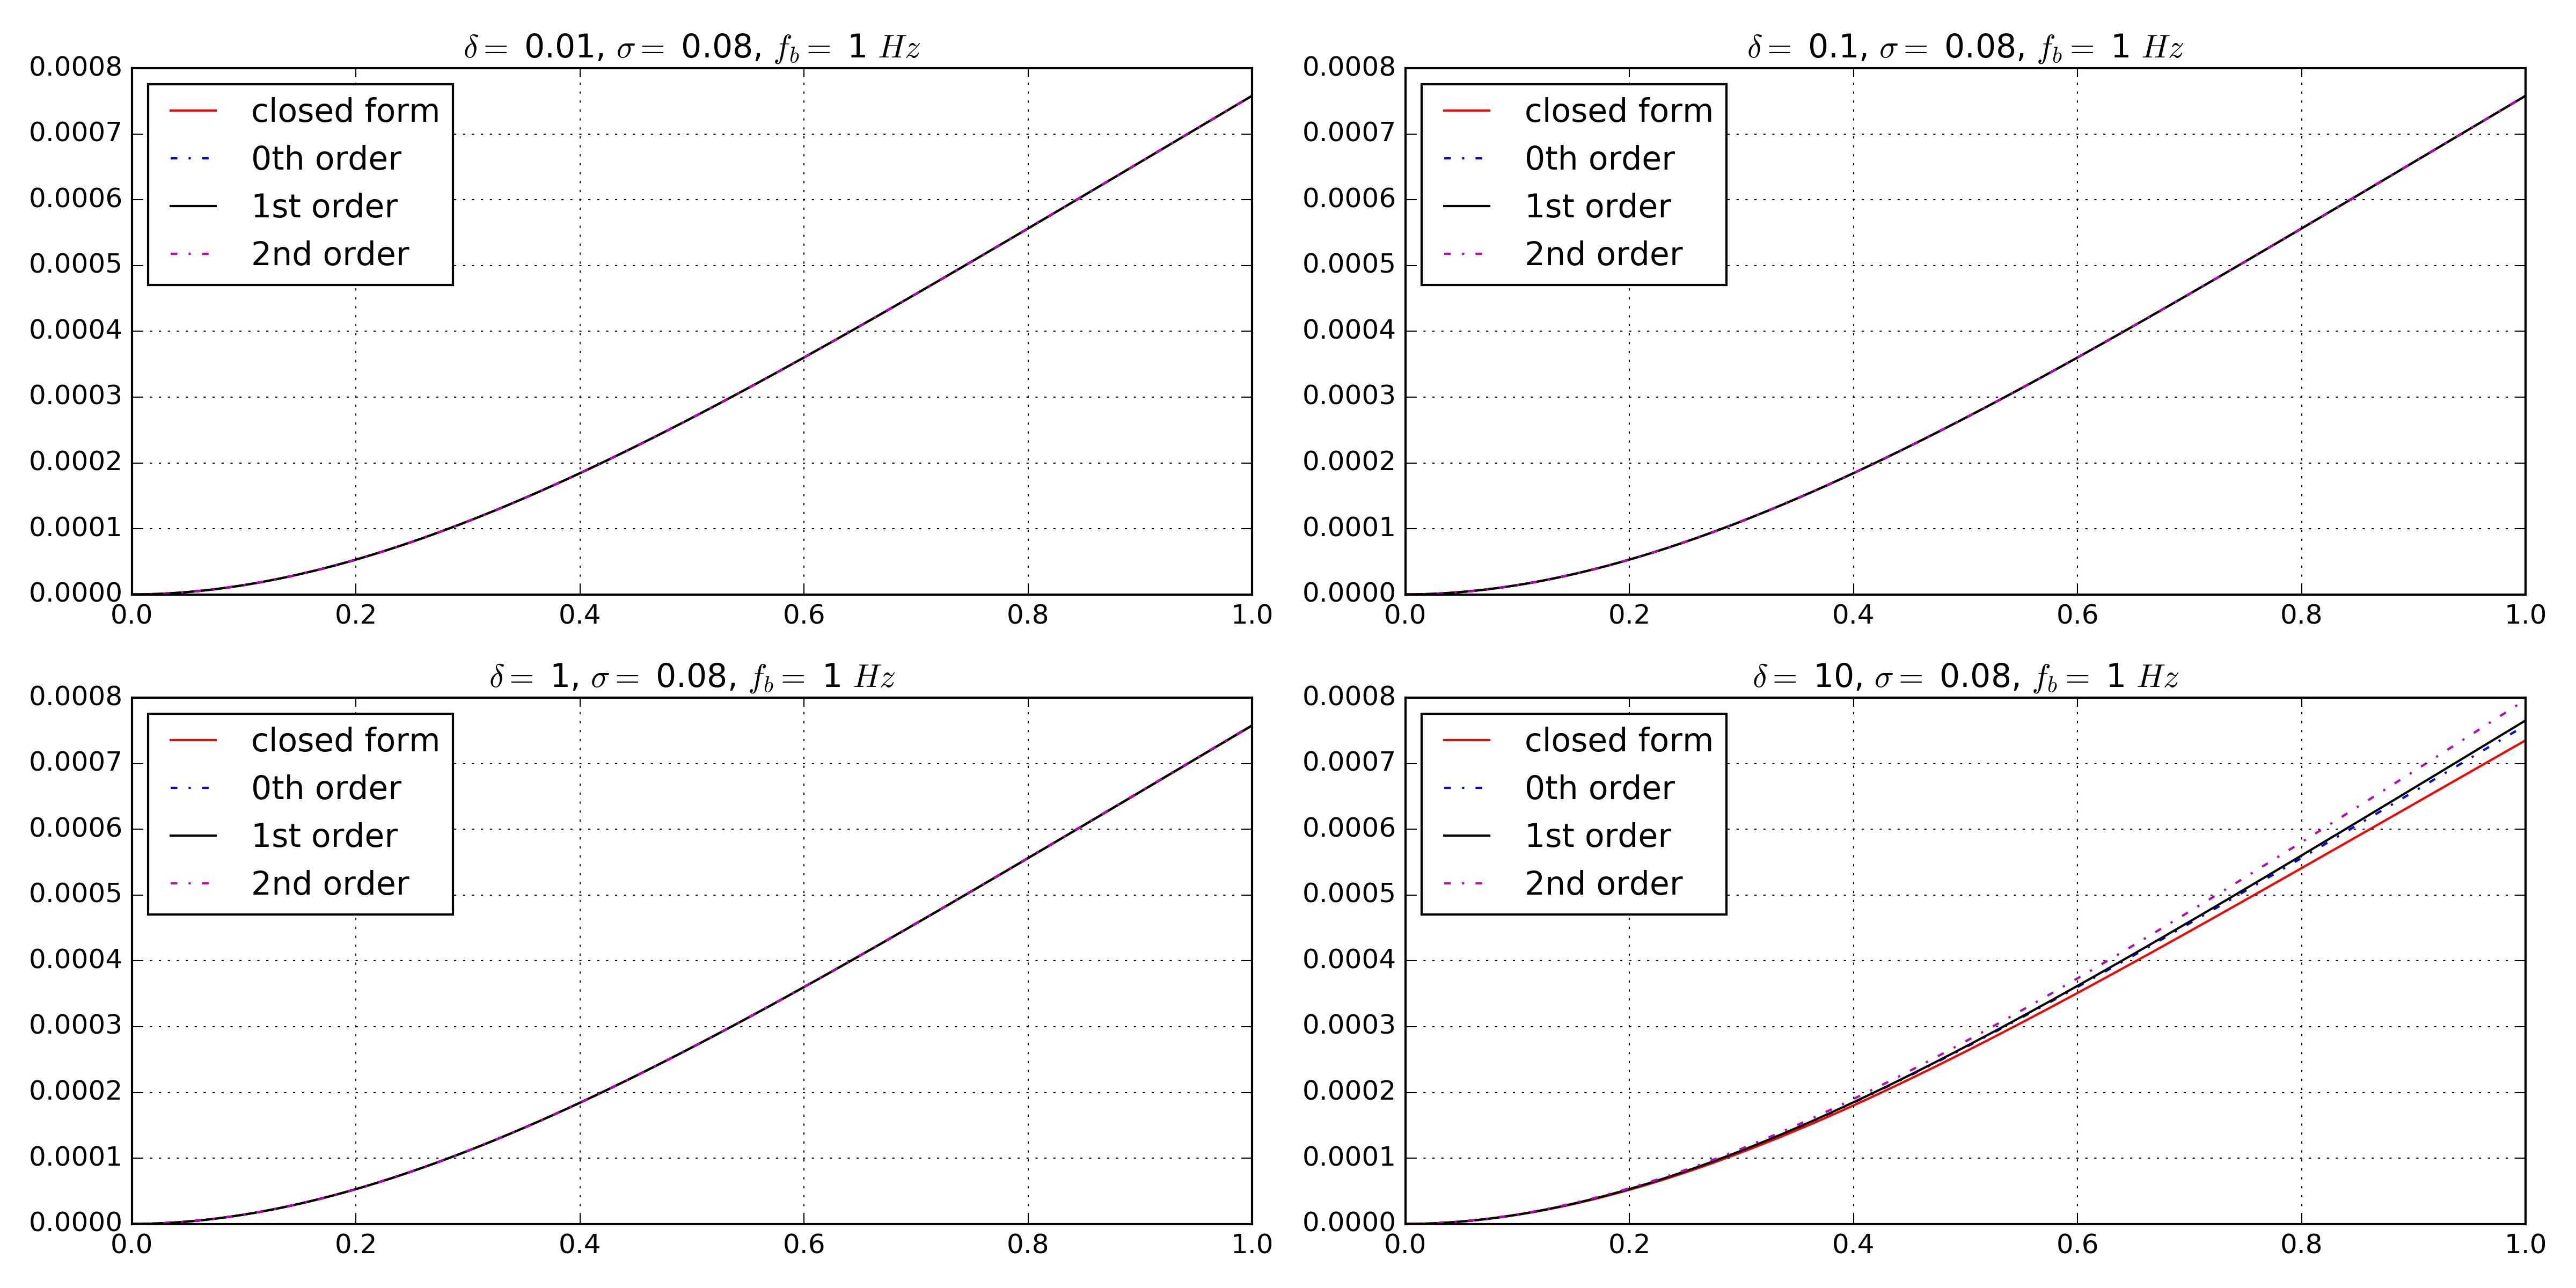
\includegraphics[width=\textwidth]{./img_eig_asy/fig_sol_analytic_disp_cmp_fr001}
    \caption{Comparison for the different orders of asymptotic expansion for the dimensionless relative displacement function $u_\delta(z)$.}
    \label{fig:fig_sol_analytic_disp_cmp_fr001}
\end{figure}



Notice from Figure~\ref{fig:fig_sol_analytic_perf_vs_fr} that the first mode resonant frequency for the device is around $45\ Hz$. It is seen from these results that a smaller value of $\delta$ results in a better approximation, whatever the value of $f_b$. This is consistent with the philosophy behind asymptotic expansion. Besides, for the frequency away from the resonant frequency, the approximation results are relatively accurate in the range of $\delta \leq 0.1$ depending on the value of $f_b$. While when the base excitation frequency $f_b$ is close to a resonance, for example $f_b = 45\ Hz$, the approximation results are not accurate even at the value of $\delta = 0.01$. That is to say, the asymptotic expansion in terms of $\delta$ is not uniform with respect to parameter $\sigma$. Especially, the existence of resonance actually restrict the behavior of the asymptotic expansion. Around the resonance the expansion will show low accuracy, while away from the resonance, the expansion accuracy is easily retained. Nonetheless, for commonly used piezoelectric materials and energy harvesting device configuration, the value of $\delta$ is usually in the range of $10^{-2}$. Hence, it is generally validated to use the asymptotic expansion method to approximate the dimensionless displacement function $u(z;\delta)$. Furthermore, in view of the approximating performances of the asymptotic expansions to different orders, it suffices to keep only the $0th$ order terms. Then, we have that 
\begin{equation}
    u(z;\delta) \approx u^{(0)}(z) = A_0 \cos{\sqrt{\sigma}z} + B_0 \sin{\sqrt{\sigma}z} + C_0 \cosh{\sqrt{\sigma}z} + D_0 \sinh{\sqrt{\sigma}z} - 1.
\end{equation}


\begin{figure}[!htbp]
    \centering
    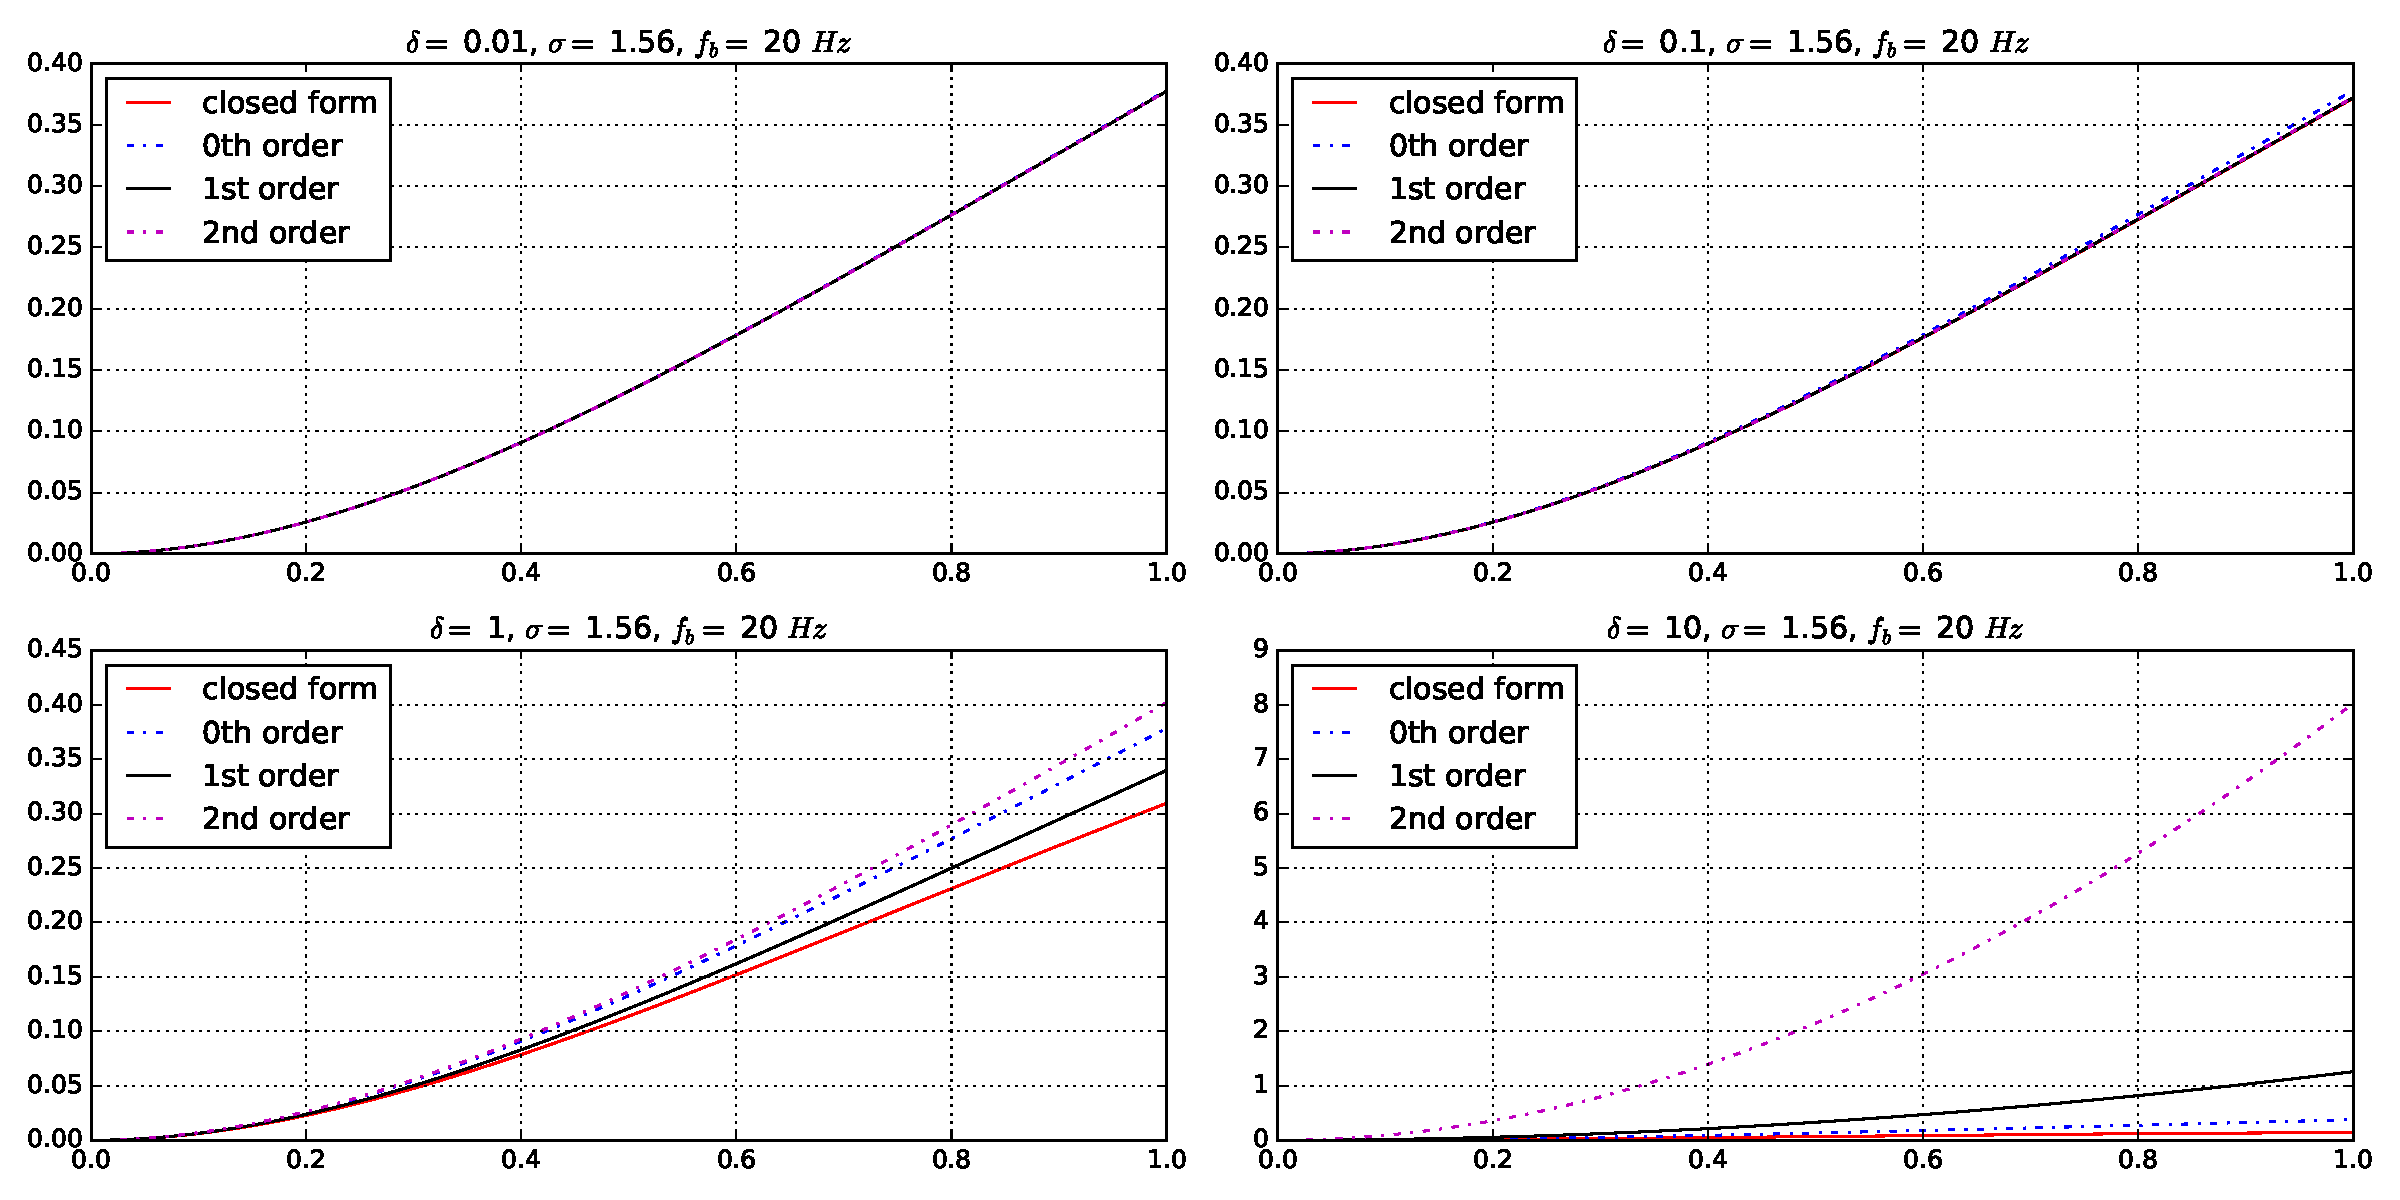
\includegraphics[width=\textwidth]{./img_eig_asy/fig_sol_analytic_disp_cmp_fr020}
    \caption{Comparison for the different orders of asymptotic expansion for the dimensionless relative displacement function $u_\delta(z)$.}
    \label{fig:fig_sol_analytic_disp_cmp_fr020}
\end{figure}


This is exactly the displacement function of a pure elastic cantilever beam. It means that for most piezoelectric energy harvesting devices, due to the fact that the electromechanical coupling factor is relatively small, the displacement function is not much affected. In this way, we have indeed uncoupled the electrical part and elastic part of a piezoelectric energy harvesting device. It should be noted that the approximation is not valid near the resonant points.





\begin{figure}[!htbp]
    \centering
    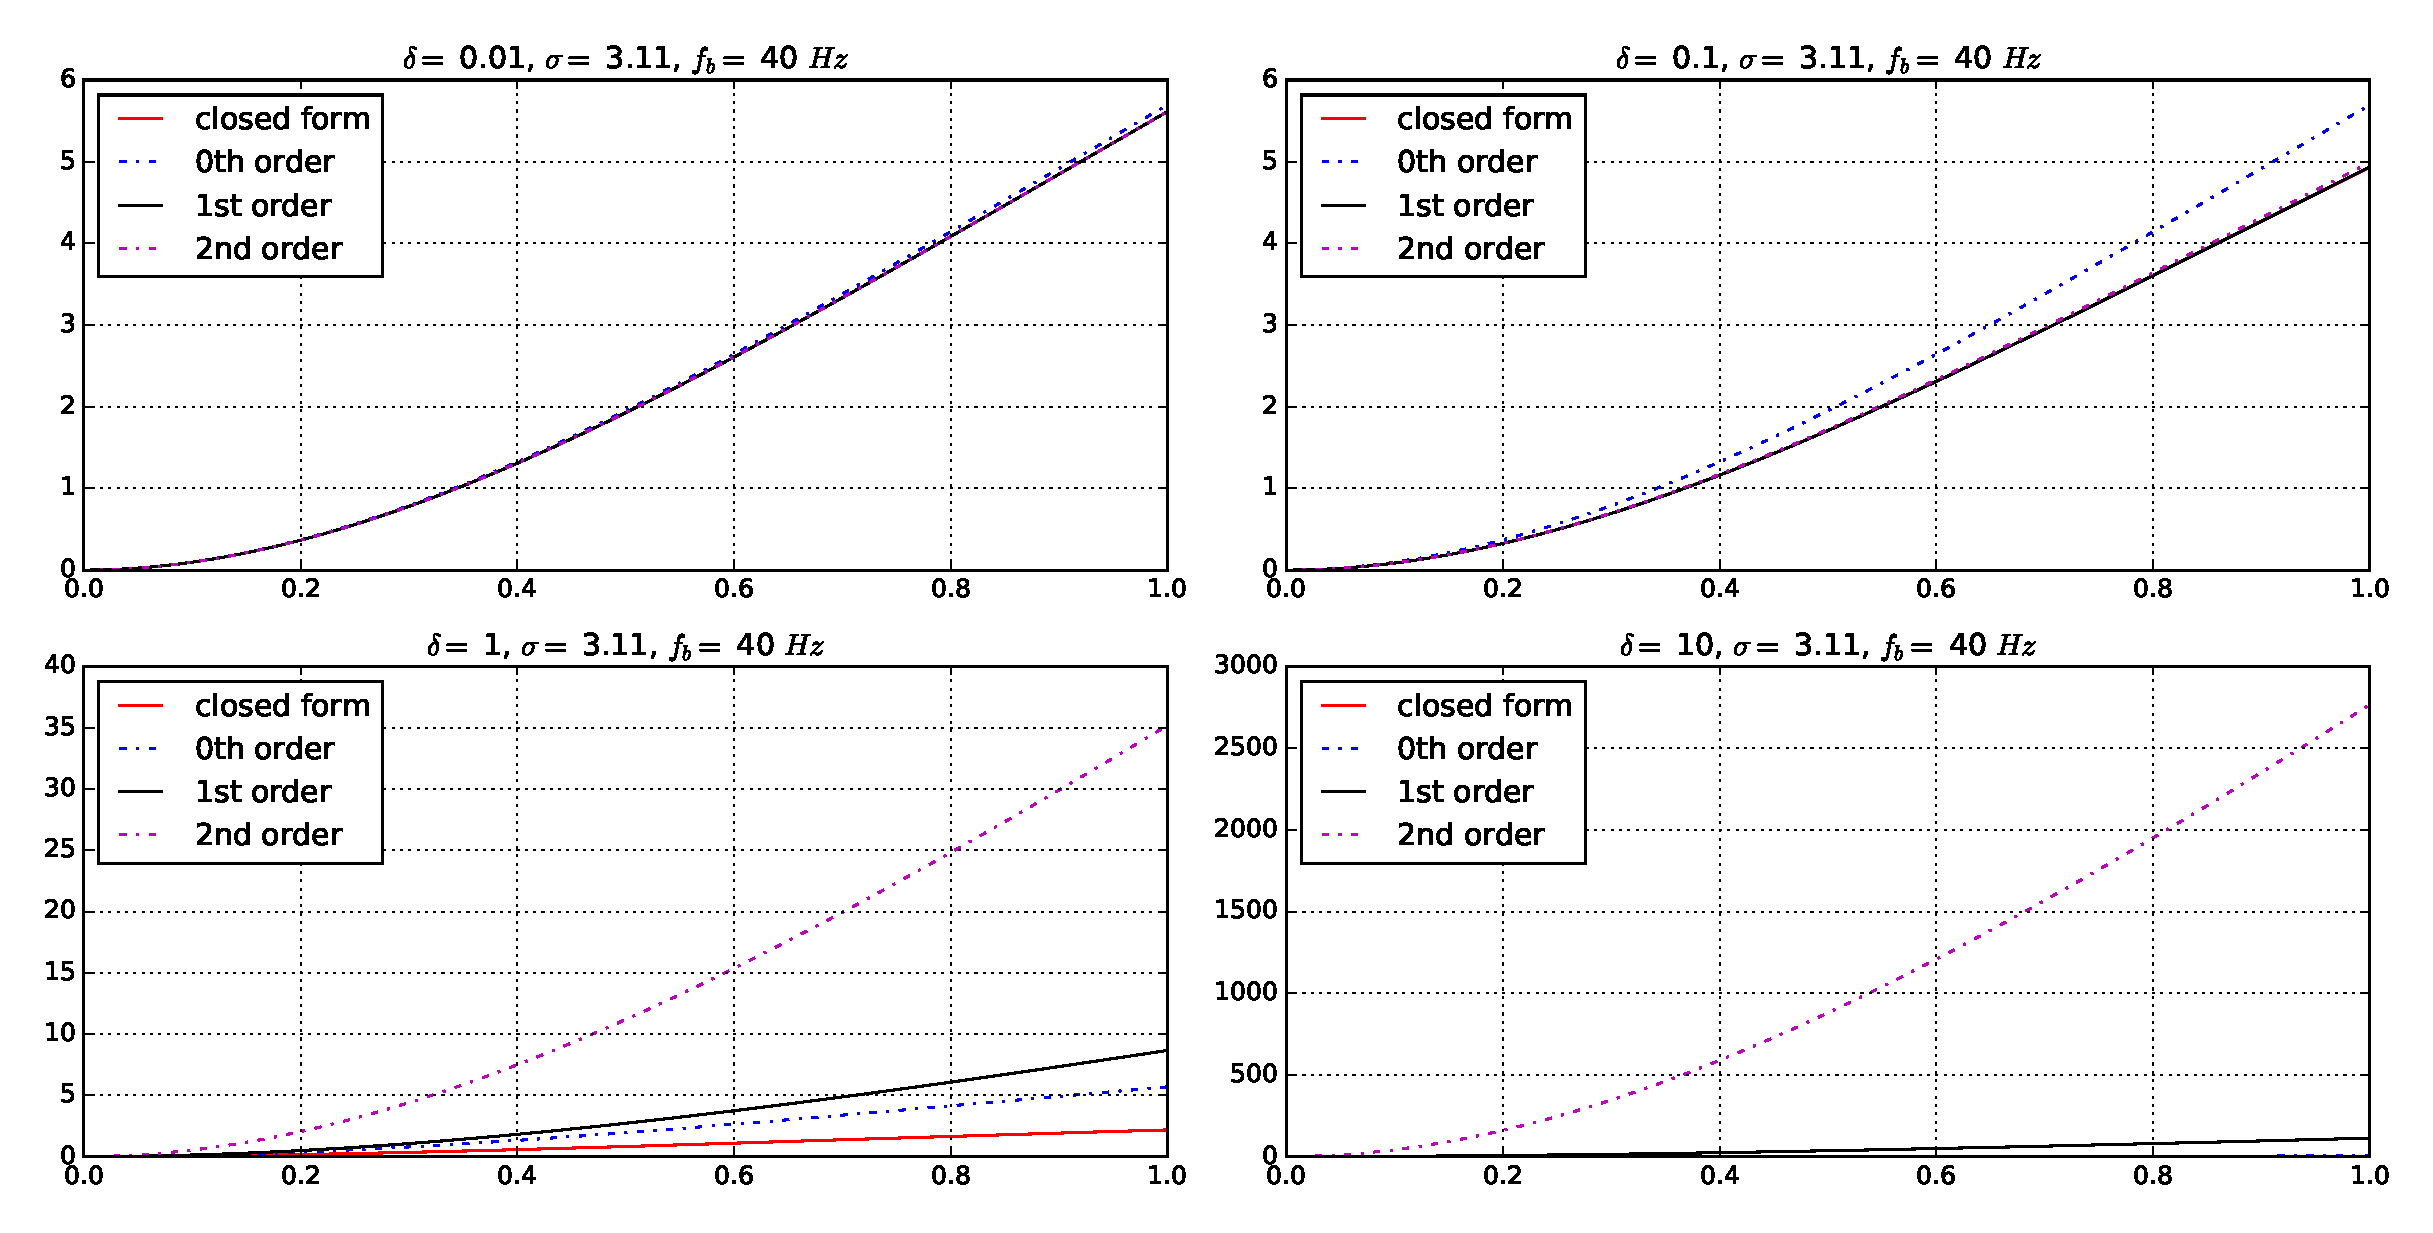
\includegraphics[width=\textwidth]{./img_eig_asy/fig_sol_analytic_disp_cmp_fr040}
    \caption{Comparison for the different orders of asymptotic expansion for the dimensionless relative displacement function $u_\delta(z)$.}
    \label{fig:fig_sol_analytic_disp_cmp_fr040}
\end{figure}


\begin{figure}[!htbp]
    \centering
    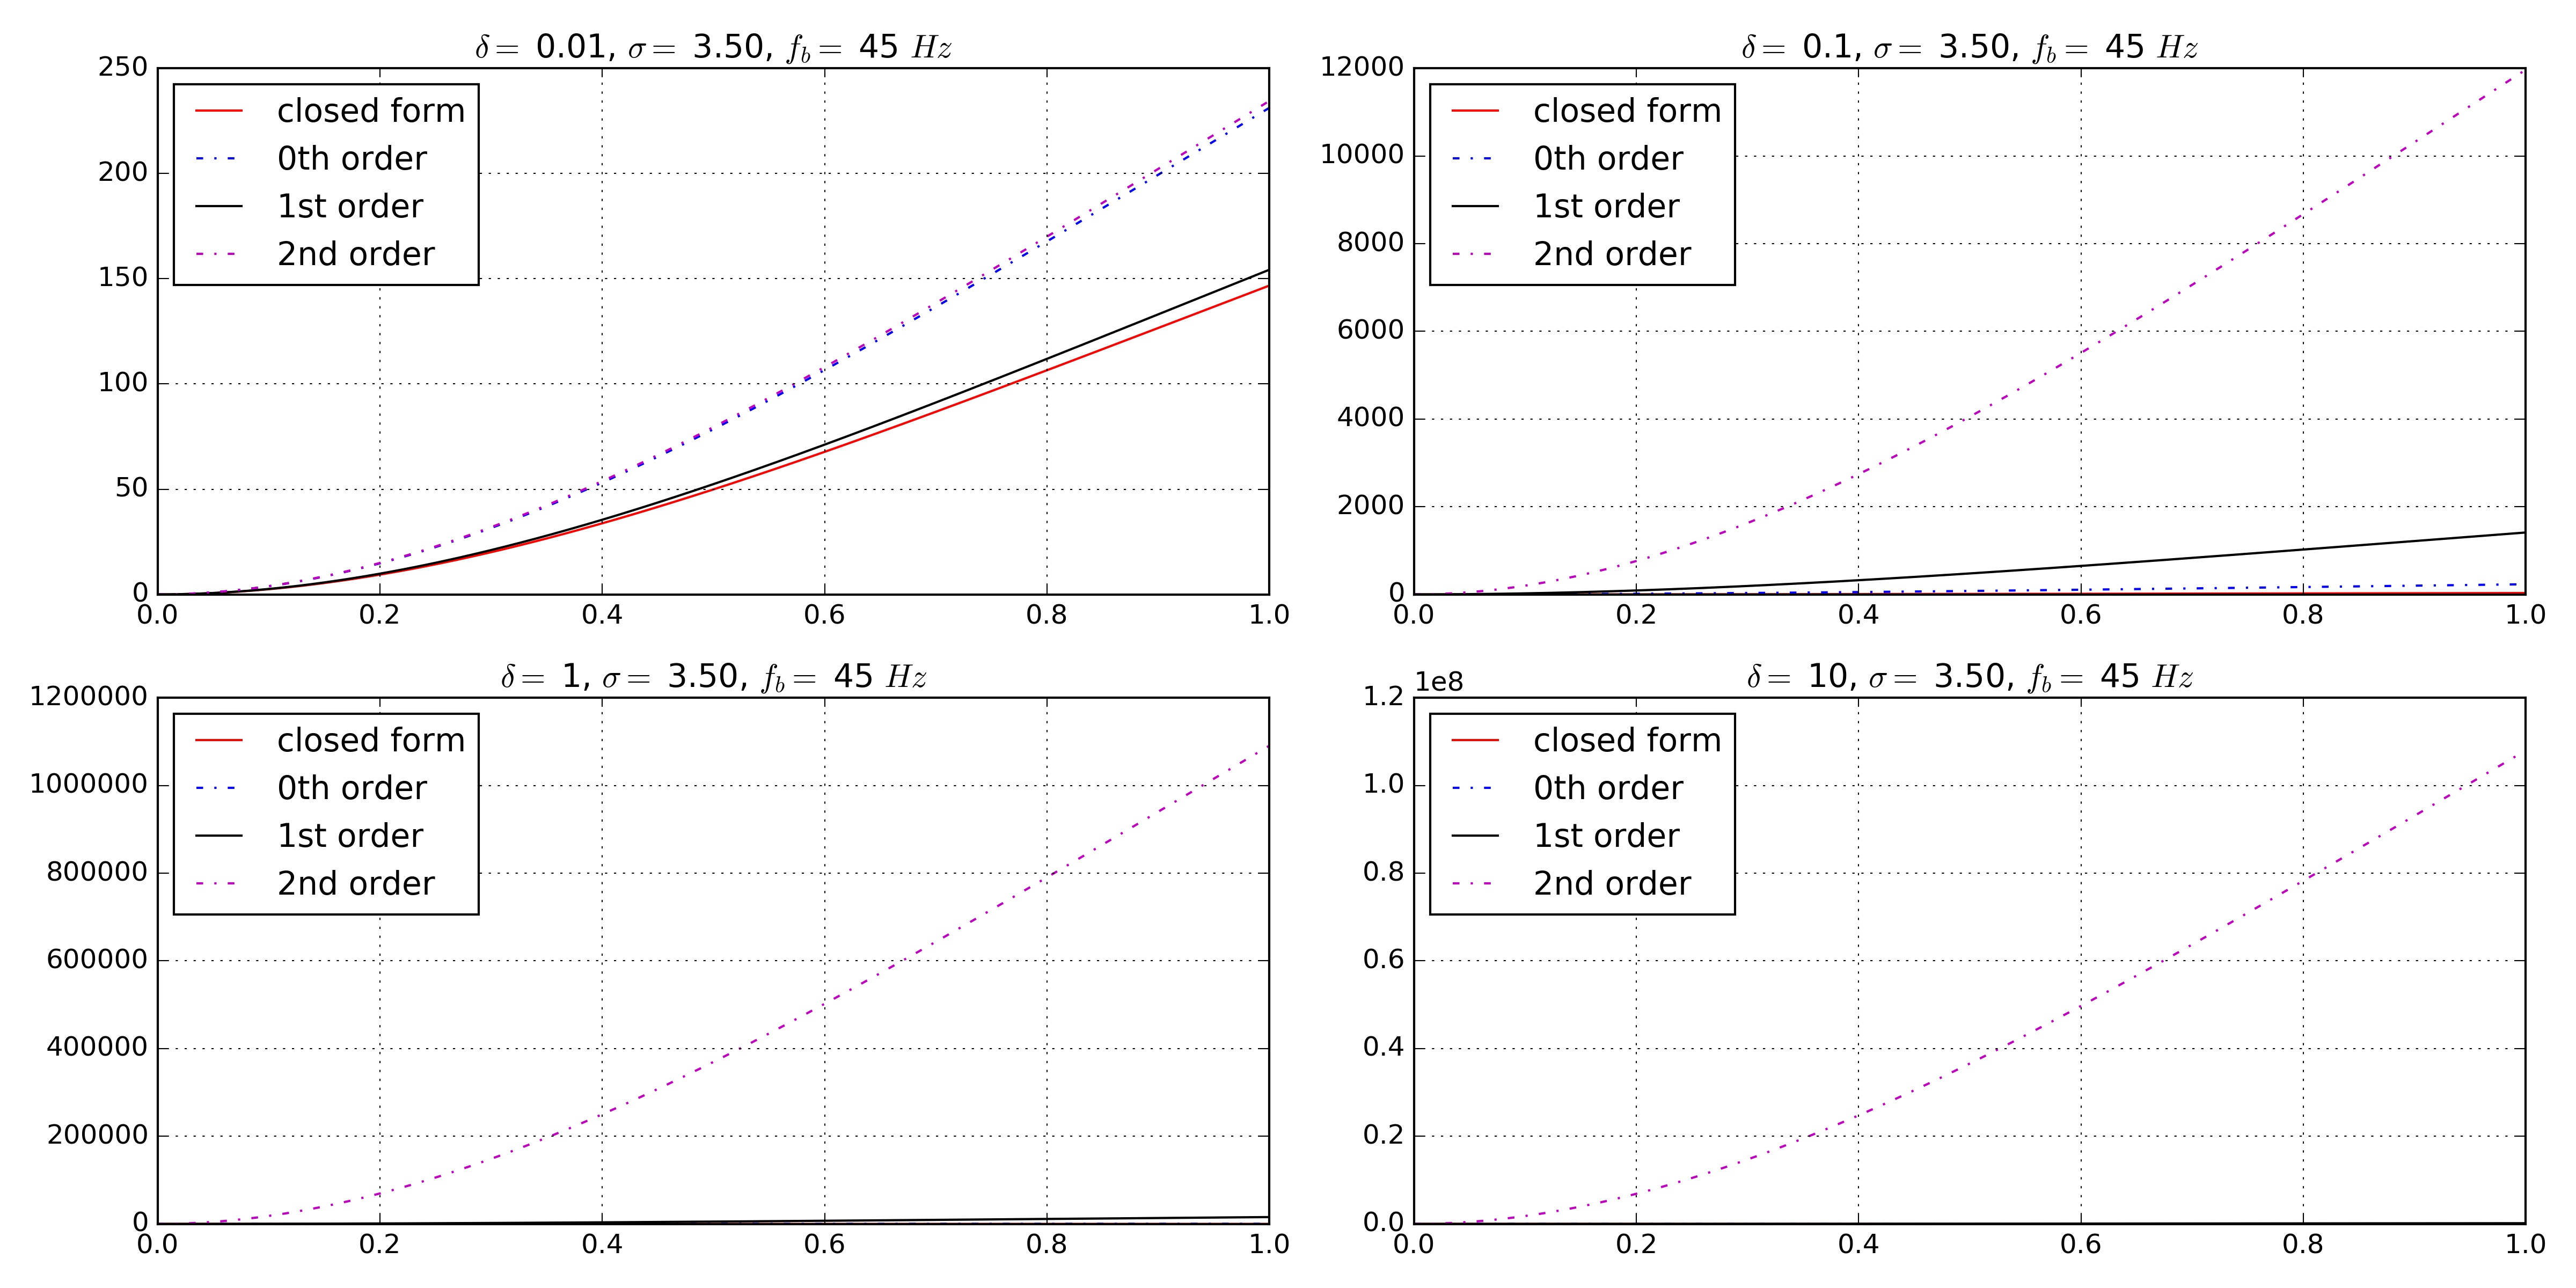
\includegraphics[width=\textwidth]{./img_eig_asy/fig_sol_analytic_disp_cmp_fr045}
    \caption{Comparison for the different orders of asymptotic expansion for the dimensionless relative displacement function $u_\delta(z)$.}
    \label{fig:fig_sol_analytic_disp_cmp_fr045}
\end{figure}


\begin{figure}[!htbp]
    \centering
    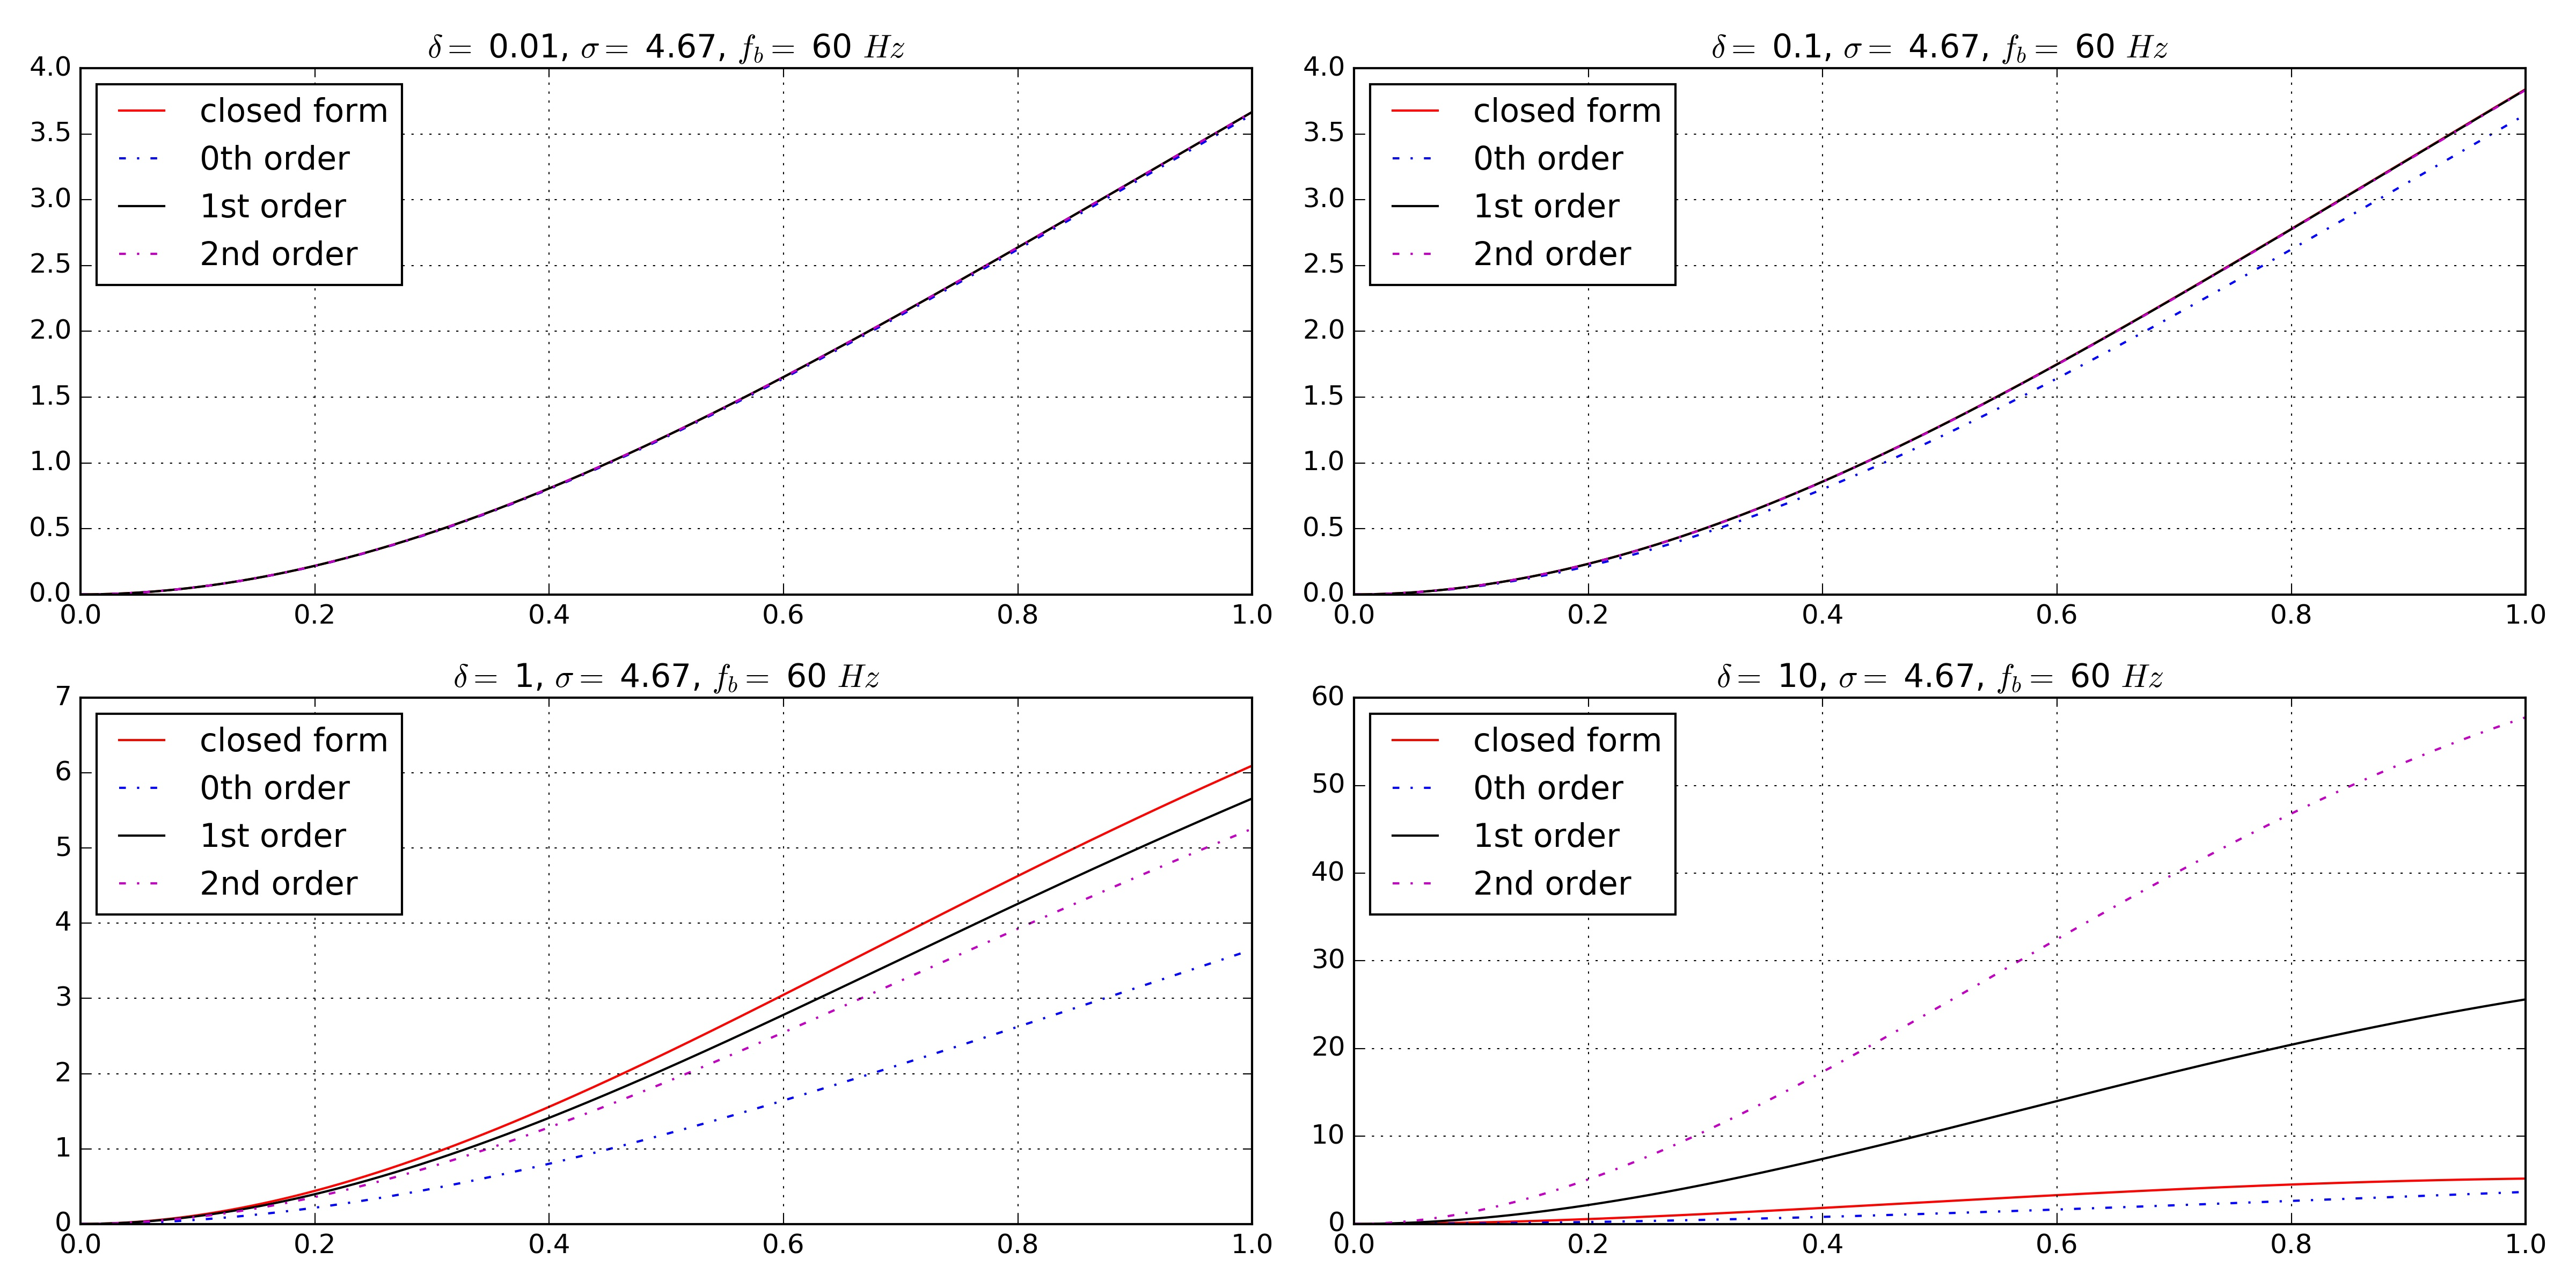
\includegraphics[width=\textwidth]{./img_eig_asy/fig_sol_analytic_disp_cmp_fr060}
    \caption{Comparison for the different orders of asymptotic expansion for the dimensionless relative displacement function $u_\delta(z)$.}
    \label{fig:fig_sol_analytic_disp_cmp_fr060}
\end{figure}


\begin{figure}[!htbp]
    \centering
    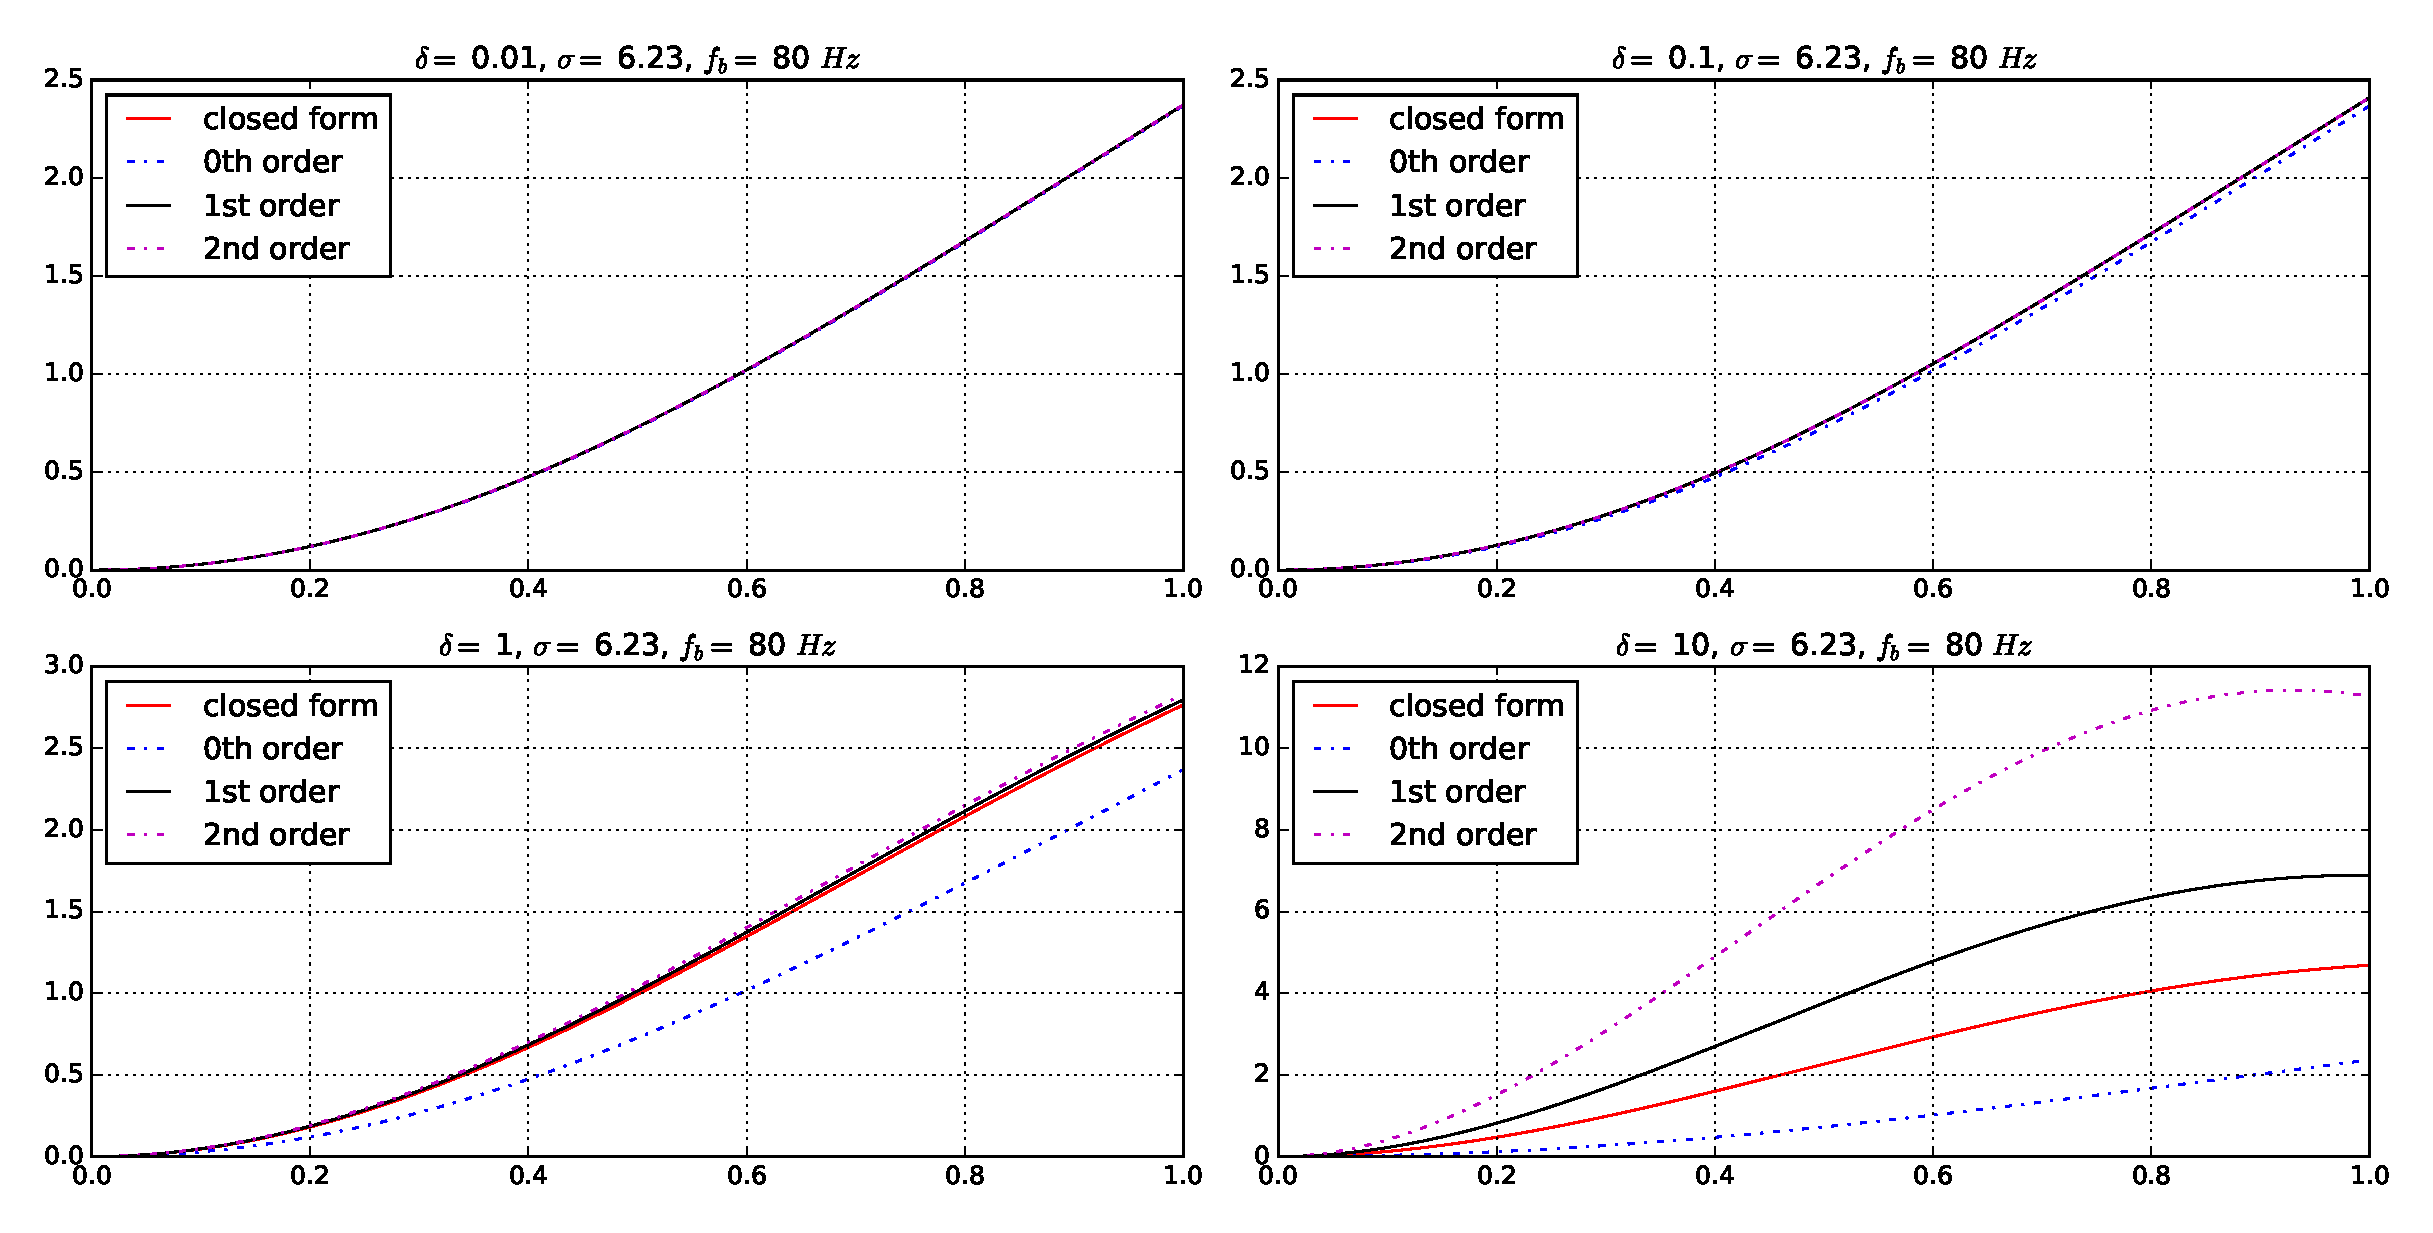
\includegraphics[width=\textwidth]{./img_eig_asy/fig_sol_analytic_disp_cmp_fr080}
    \caption{Comparison for the different orders of asymptotic expansion for the dimensionless relative displacement function $u_\delta(z)$.}
    \label{fig:fig_sol_analytic_disp_cmp_fr080}
\end{figure}


\begin{figure}[!htbp]
    \centering
    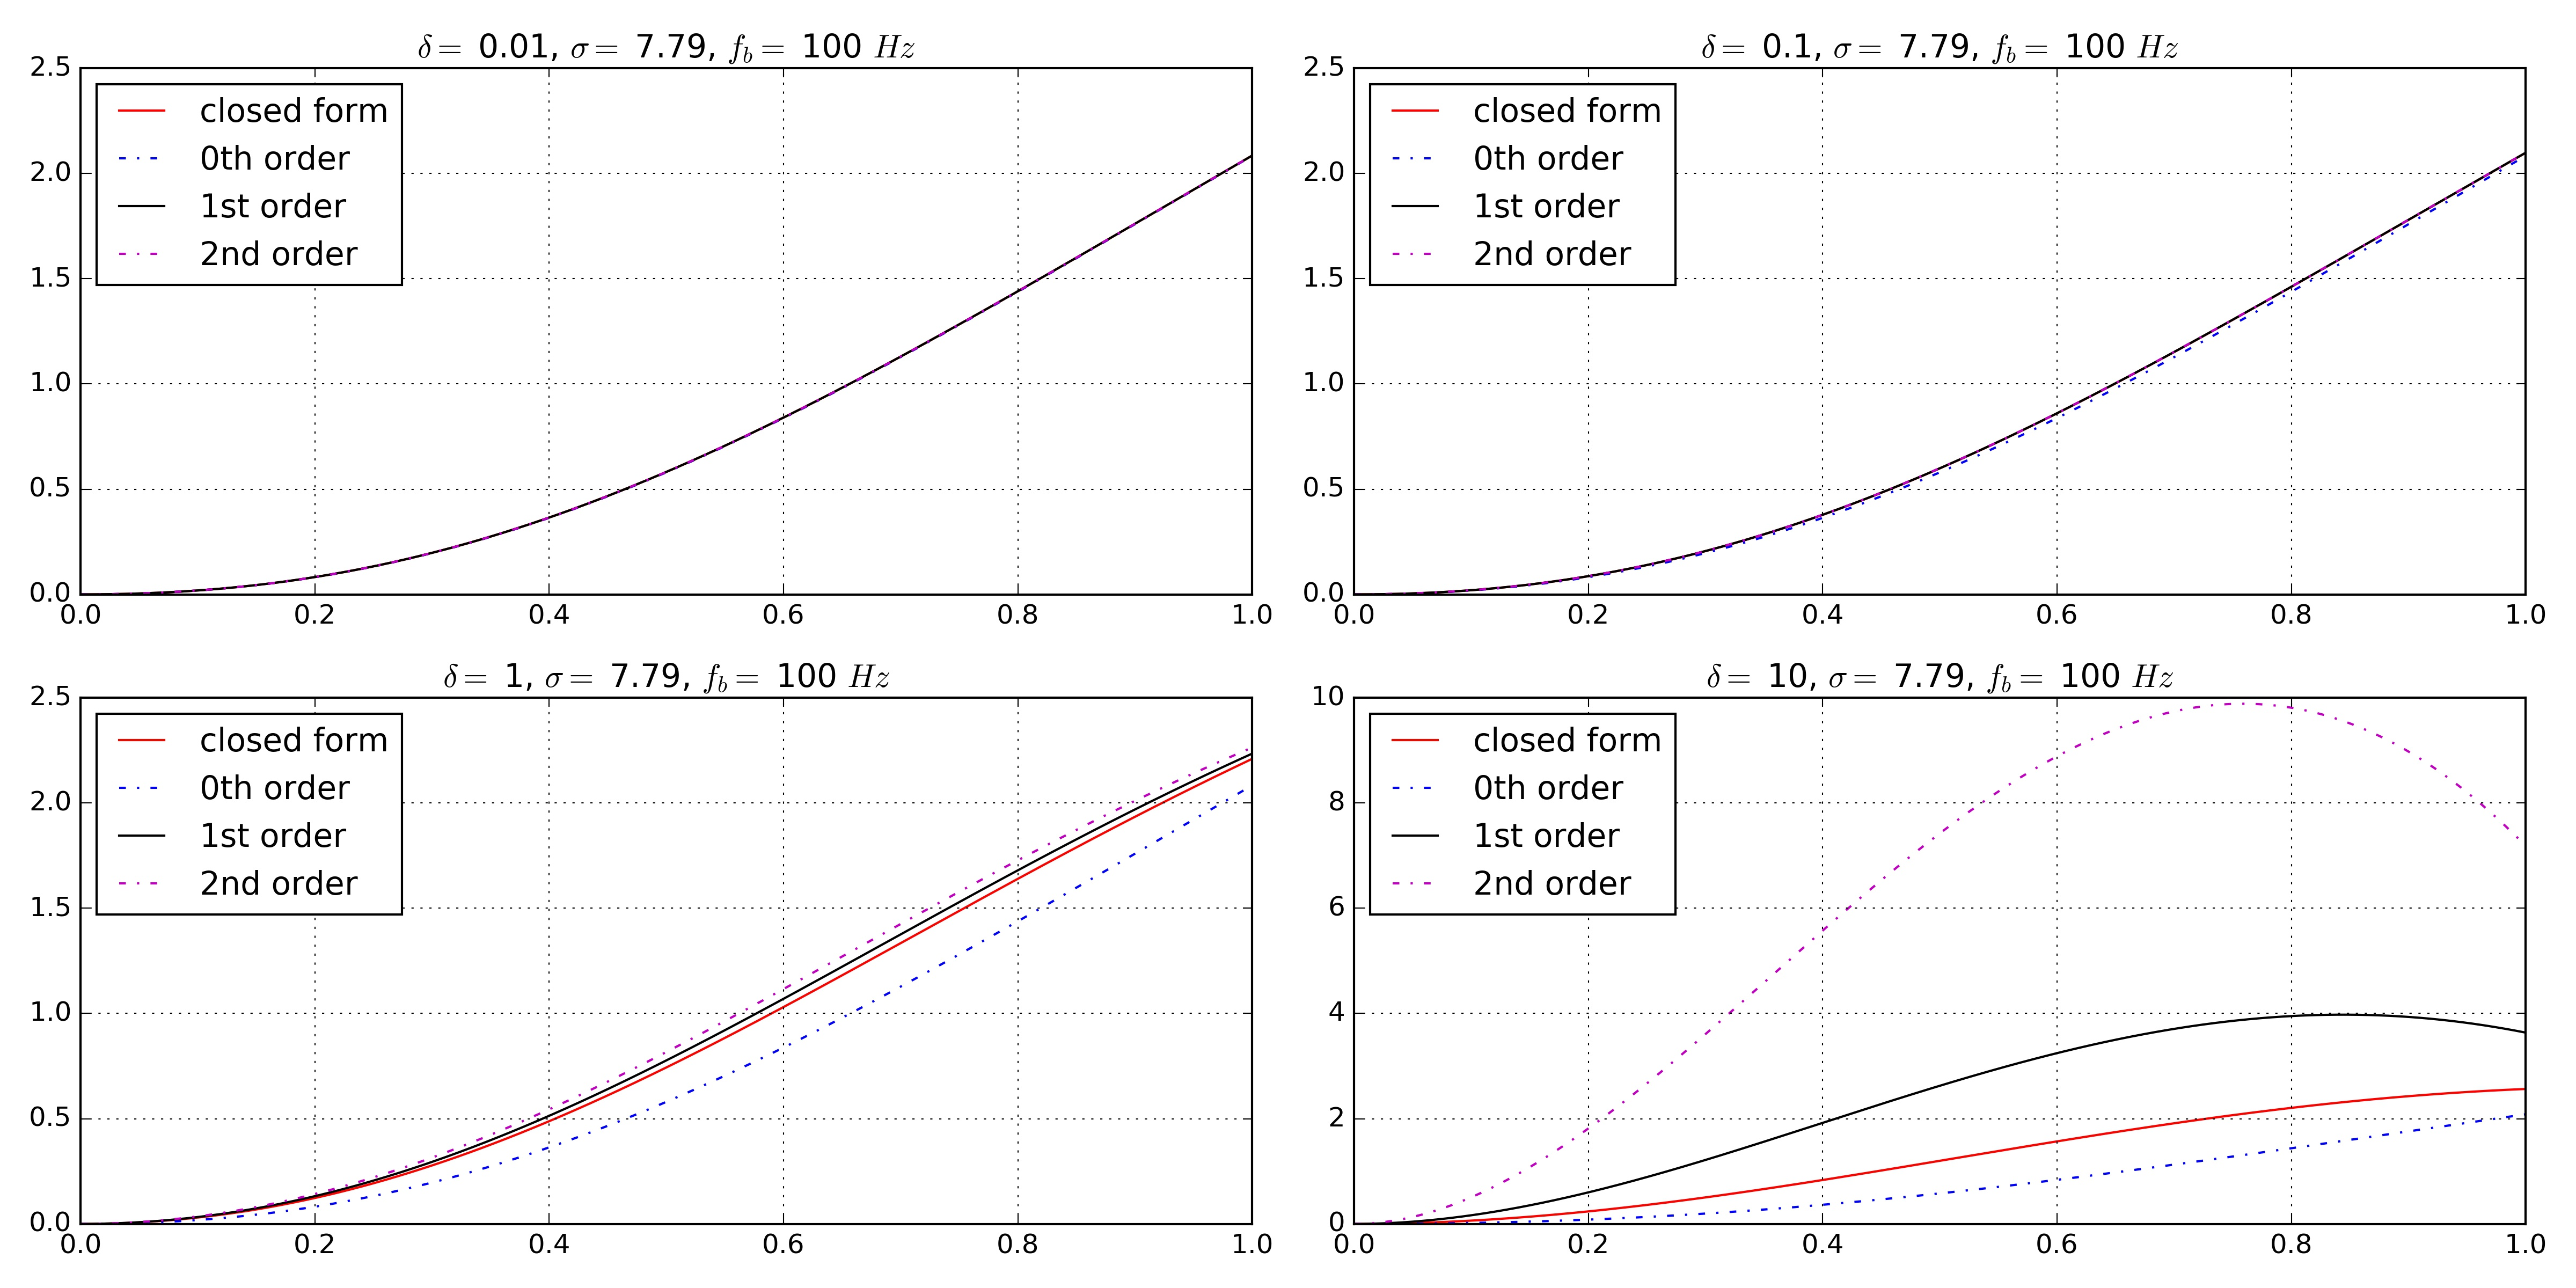
\includegraphics[width=\textwidth]{./img_eig_asy/fig_sol_analytic_disp_cmp_fr100}
    \caption{Comparison for the different orders of asymptotic expansion for the dimensionless relative displacement function $u_\delta(z)$.}
    \label{fig:fig_sol_analytic_disp_cmp_fr100}
\end{figure}


Theoretically, the first order derivative of the dimensionless relative displacement function $u(z;\delta)$ is 
\begin{equation}
    u^{\prime}(z;\delta) = \sigma^{1/2} \left( - A_\delta \sin{\sqrt{\sigma}z} + B_\delta \cos{\sqrt{\sigma}z} + C_\delta \sinh{\sqrt{\sigma}z} + D_\delta \cosh{\sqrt{\sigma}z} \right).
\end{equation}
\begin{equation}
    \chi_p = u_1^\prime(1) = \frac{ \sqrt{\sigma} \left( \sinh\sqrt{\sigma} - \sin\sqrt{\sigma} \right) }{ 1 + \cos\sqrt{\sigma } \cosh\sqrt{\sigma } + \frac{j \beta \sqrt{\sigma}}{ 1+ j \beta \sigma } \delta \left( \cos\sqrt{\sigma } \sinh\sqrt{\sigma } + \sin\sqrt{\sigma } \cosh\sqrt{\sigma } \right) }.
    \label{eq:eq_peh_perfs_compact_form_end_ders1}
\end{equation}
The value of this function at the free end ($z=1$) is just the output index $\chi_p$ according to equation (\ref{eq:eq_peh_perfs_compact_form_end_ders}). To see the influences of $\delta$ and $f_b$, therefore $\sigma$, upon $\chi_p$, we firstly calculate the values of $\chi_p$ for different values of $\delta$ by fixing the value of $f_b$ to be some discrete values. The results are shown in Figure~\ref{fig:fig_sol_analytic_out_index_vs_delta}. 


\begin{figure}[!htbp]
    \centering
    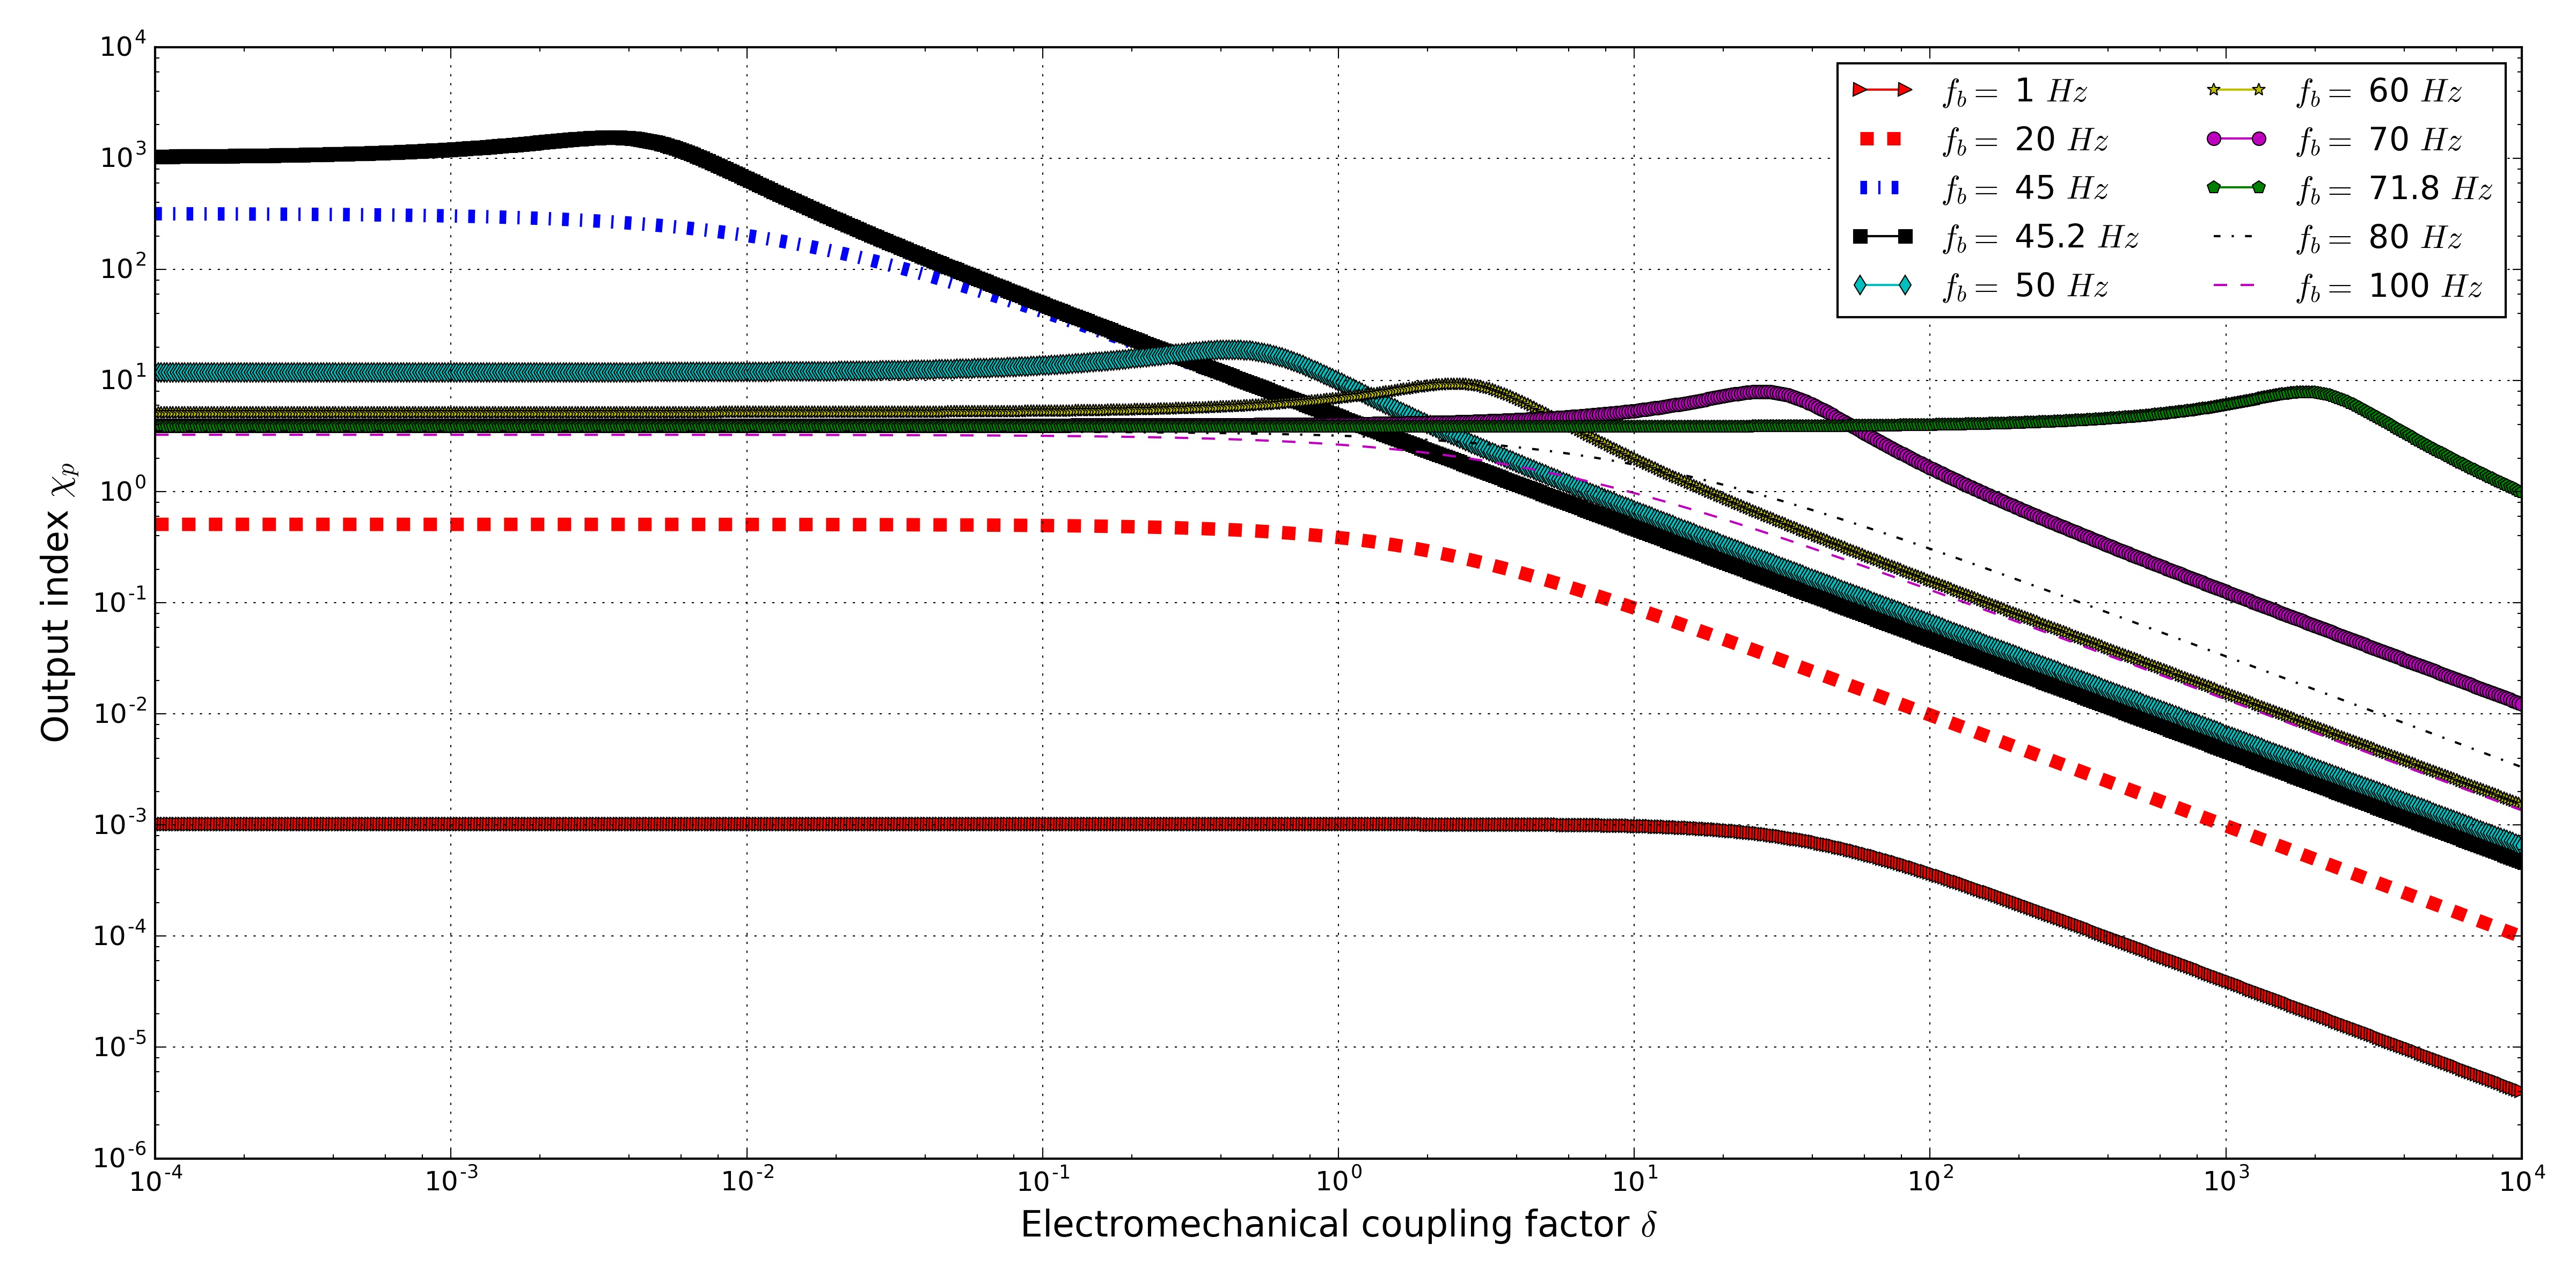
\includegraphics[width=\textwidth]{./img_eig_asy/fig_sol_analytic_out_index_vs_delta}
    \caption{Output index $\chi_p$ as a function of electromechanical coupling factor $\delta$ at different values of base excitation frequency $f_b$.}
    \label{fig:fig_sol_analytic_out_index_vs_delta}
\end{figure}


It is seen that the dependence of $\chi_p$ upon $\delta$ shows two different modes in the frequency range of $1\ - \ 100\ Hz$. For the frequencies of $45.2\ Hz \leq f_b \leq 71.8\ Hz$, a peak corresponding to a critical value of $\delta_p$ is present in the considered range of $\delta$. When $\delta$ is smaller than $\delta_p$, the output index $\chi_p$ increases along with $\delta$, and when $\delta$ is larger than $\delta_p$, the output index $\chi_p$ decreases with the increase of $\delta$. On the other hand, for the frequency range of $f_b \leq 45\ Hz$ or $f_b \geq 80\ Hz$, the output index $\chi_p$ shows a monotonic decrease with respect to the increase $\delta$.


\begin{figure}[!htbp]
    \centering
    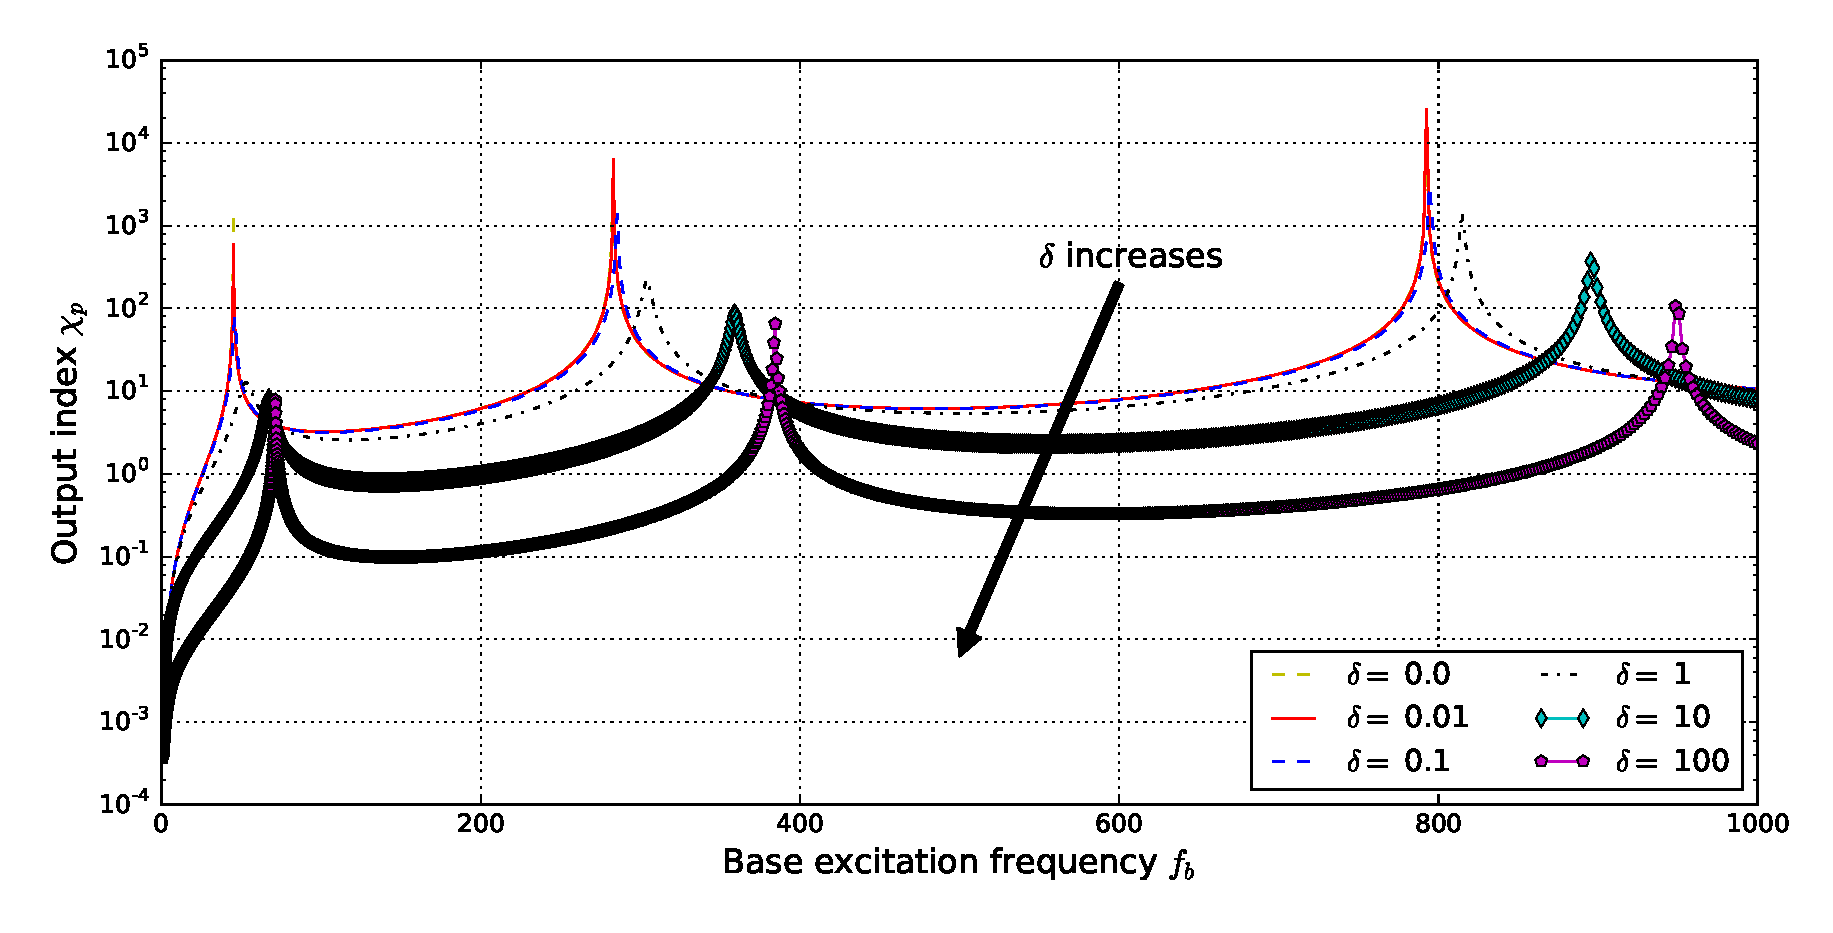
\includegraphics[width=\textwidth]{./img_eig_asy/fig_sol_analytic_out_index_vs_fr}
    \caption{Output index $\chi_p$ as a function of base excitation frequency $f_b$ at different values of electromechanical coupling factor $\delta$.}
    \label{fig:fig_sol_analytic_out_index_vs_fr}
\end{figure}


Alternatively, by fixing the values of $\delta$ to a discrete set of numbers, we calculate the values of $\chi_p$ in relation to different values of $f_b$. This is very similar to a frequency response of the output index as a function of $\sigma$. The results are shown in Figure~\ref{fig:fig_sol_analytic_out_index_vs_fr}. It is clearly shown that with the increase of electromechanical coupling factor $\delta$, the resonant frequencies to the system increase with the increase of $\delta$. This is clearly shown in the shift to the right of the frequency response curve. Besides, we add in this figure the case where $\delta = 0.0$ as a reference. Simple comparisons show that the discrepancy between the frequency response curves related to the case of $\delta = 0$, $\delta=0.01$, and $\delta = 0.1$ is small. A direct conclusion is that for relatively small values of electromechanical coupling factor $\delta$, the output index $\chi_p$ can be approximated by 
\begin{equation}
    \chi_p \approx \frac{ \sqrt{\sigma} \left( \sinh\sqrt{\sigma} - \sin\sqrt{\sigma} \right) }{ 1 + \cos\sqrt{\sigma } \cosh\sqrt{\sigma } }.
\end{equation}

As a result, the output performance measures $\tilde{V}_p$, $\tilde{I}_p$, and $\tilde{P}_p$ can be approximated by 
\begin{equation}
    \left\{\begin{aligned}
        \tilde{V}_p &= - \frac{j \sigma \beta}{j \sigma \beta + 1} \left(\frac{\eta_b}{l_p}\right) \left(\frac{e_p}{C_p}\right) \chi_p , \\
        &= - \frac{j \sigma \beta}{j \sigma \beta + 1} \left(\frac{\eta_b}{l_p}\right) \left(\frac{e_p}{C_p}\right) \frac{ \sqrt{\sigma} \left( \sinh\sqrt{\sigma} - \sin\sqrt{\sigma} \right) }{ 1 + \cos\sqrt{\sigma } \cosh\sqrt{\sigma } } , \\
        \tilde{I}_p &=  \tilde{V}_p / R_l = - \frac{ j \sigma \beta } {j \sigma \beta + 1} \left( \frac{\eta_b}{l_p} \right) \left( \frac{e_p}{C_p R_l} \right) \chi_p , \\
        &= - \frac{ j \sigma \beta } {j \sigma \beta + 1} \left( \frac{\eta_b}{l_p} \right) \left( \frac{e_p}{C_p R_l} \right) \frac{ \sqrt{\sigma} \left( \sinh\sqrt{\sigma} - \sin\sqrt{\sigma} \right) }{ 1 + \cos\sqrt{\sigma } \cosh\sqrt{\sigma } }, \\
        \tilde{P}_p &=  \tilde{V}_p^2 / R_l = \left(\frac{\eta_b}{l_p}\right)^2 \left(\frac{e_p}{C_p}\right) \left( \frac{e_p}{C_p R_l} \right) \left( \frac{ j \sigma \beta}{ j \sigma \beta + 1 } \right)^2 \chi_p^2, \\
        &= \left(\frac{\eta_b}{l_p}\right)^2 \left(\frac{e_p}{C_p}\right) \left( \frac{e_p}{C_p R_l} \right) \left( \frac{ j \sigma \beta}{ j \sigma \beta + 1 } \right)^2 \left( \frac{ \sqrt{\sigma} \left( \sinh\sqrt{\sigma} - \sin\sqrt{\sigma} \right) }{ 1 + \cos\sqrt{\sigma } \cosh\sqrt{\sigma } } \right)^2.
    \end{aligned}\right.
    \label{eq:eq_peh_perfs_compact_form_approx}
\end{equation}


\begin{figure}[!htbp]
    \centering
    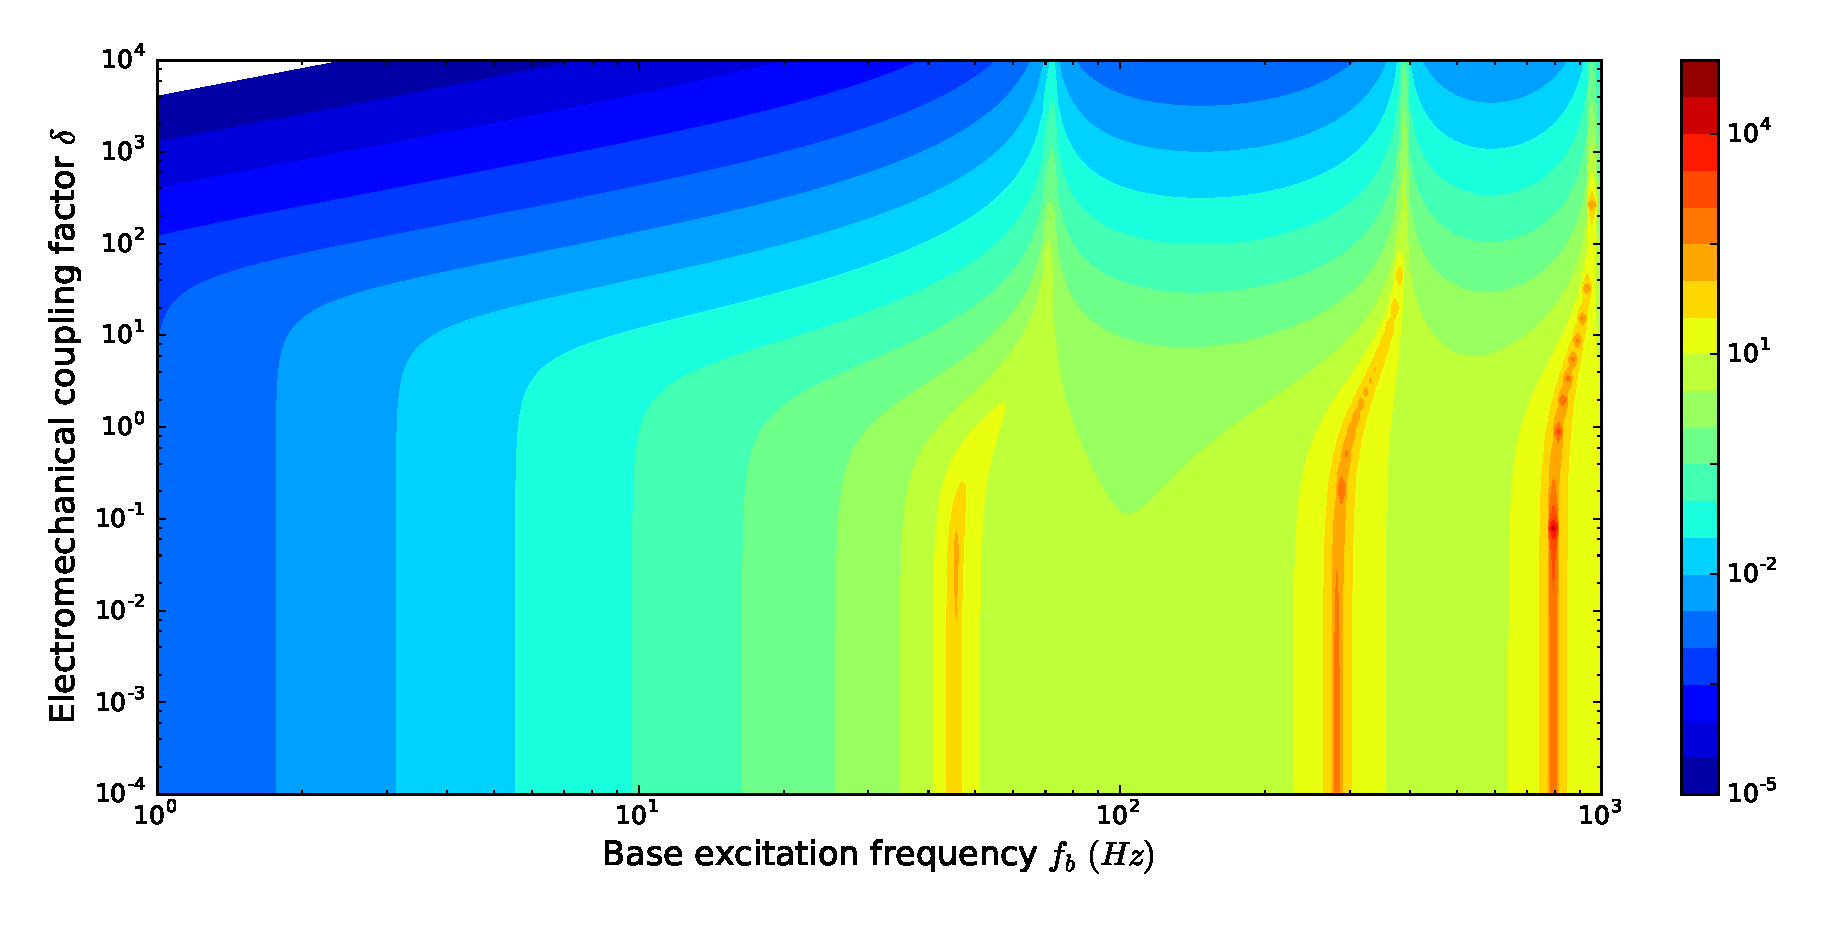
\includegraphics[width=\textwidth]{./img_eig_asy/fig_sol_analytic_out_index_contour}
    \caption{Output index $\chi_p$ as a function of base excitation frequency $f_b$ and electromechanical coupling factor $\delta$.}
    \label{fig:fig_sol_analytic_out_index_contour}
\end{figure}



\begin{figure}[!htbp]
    \centering
    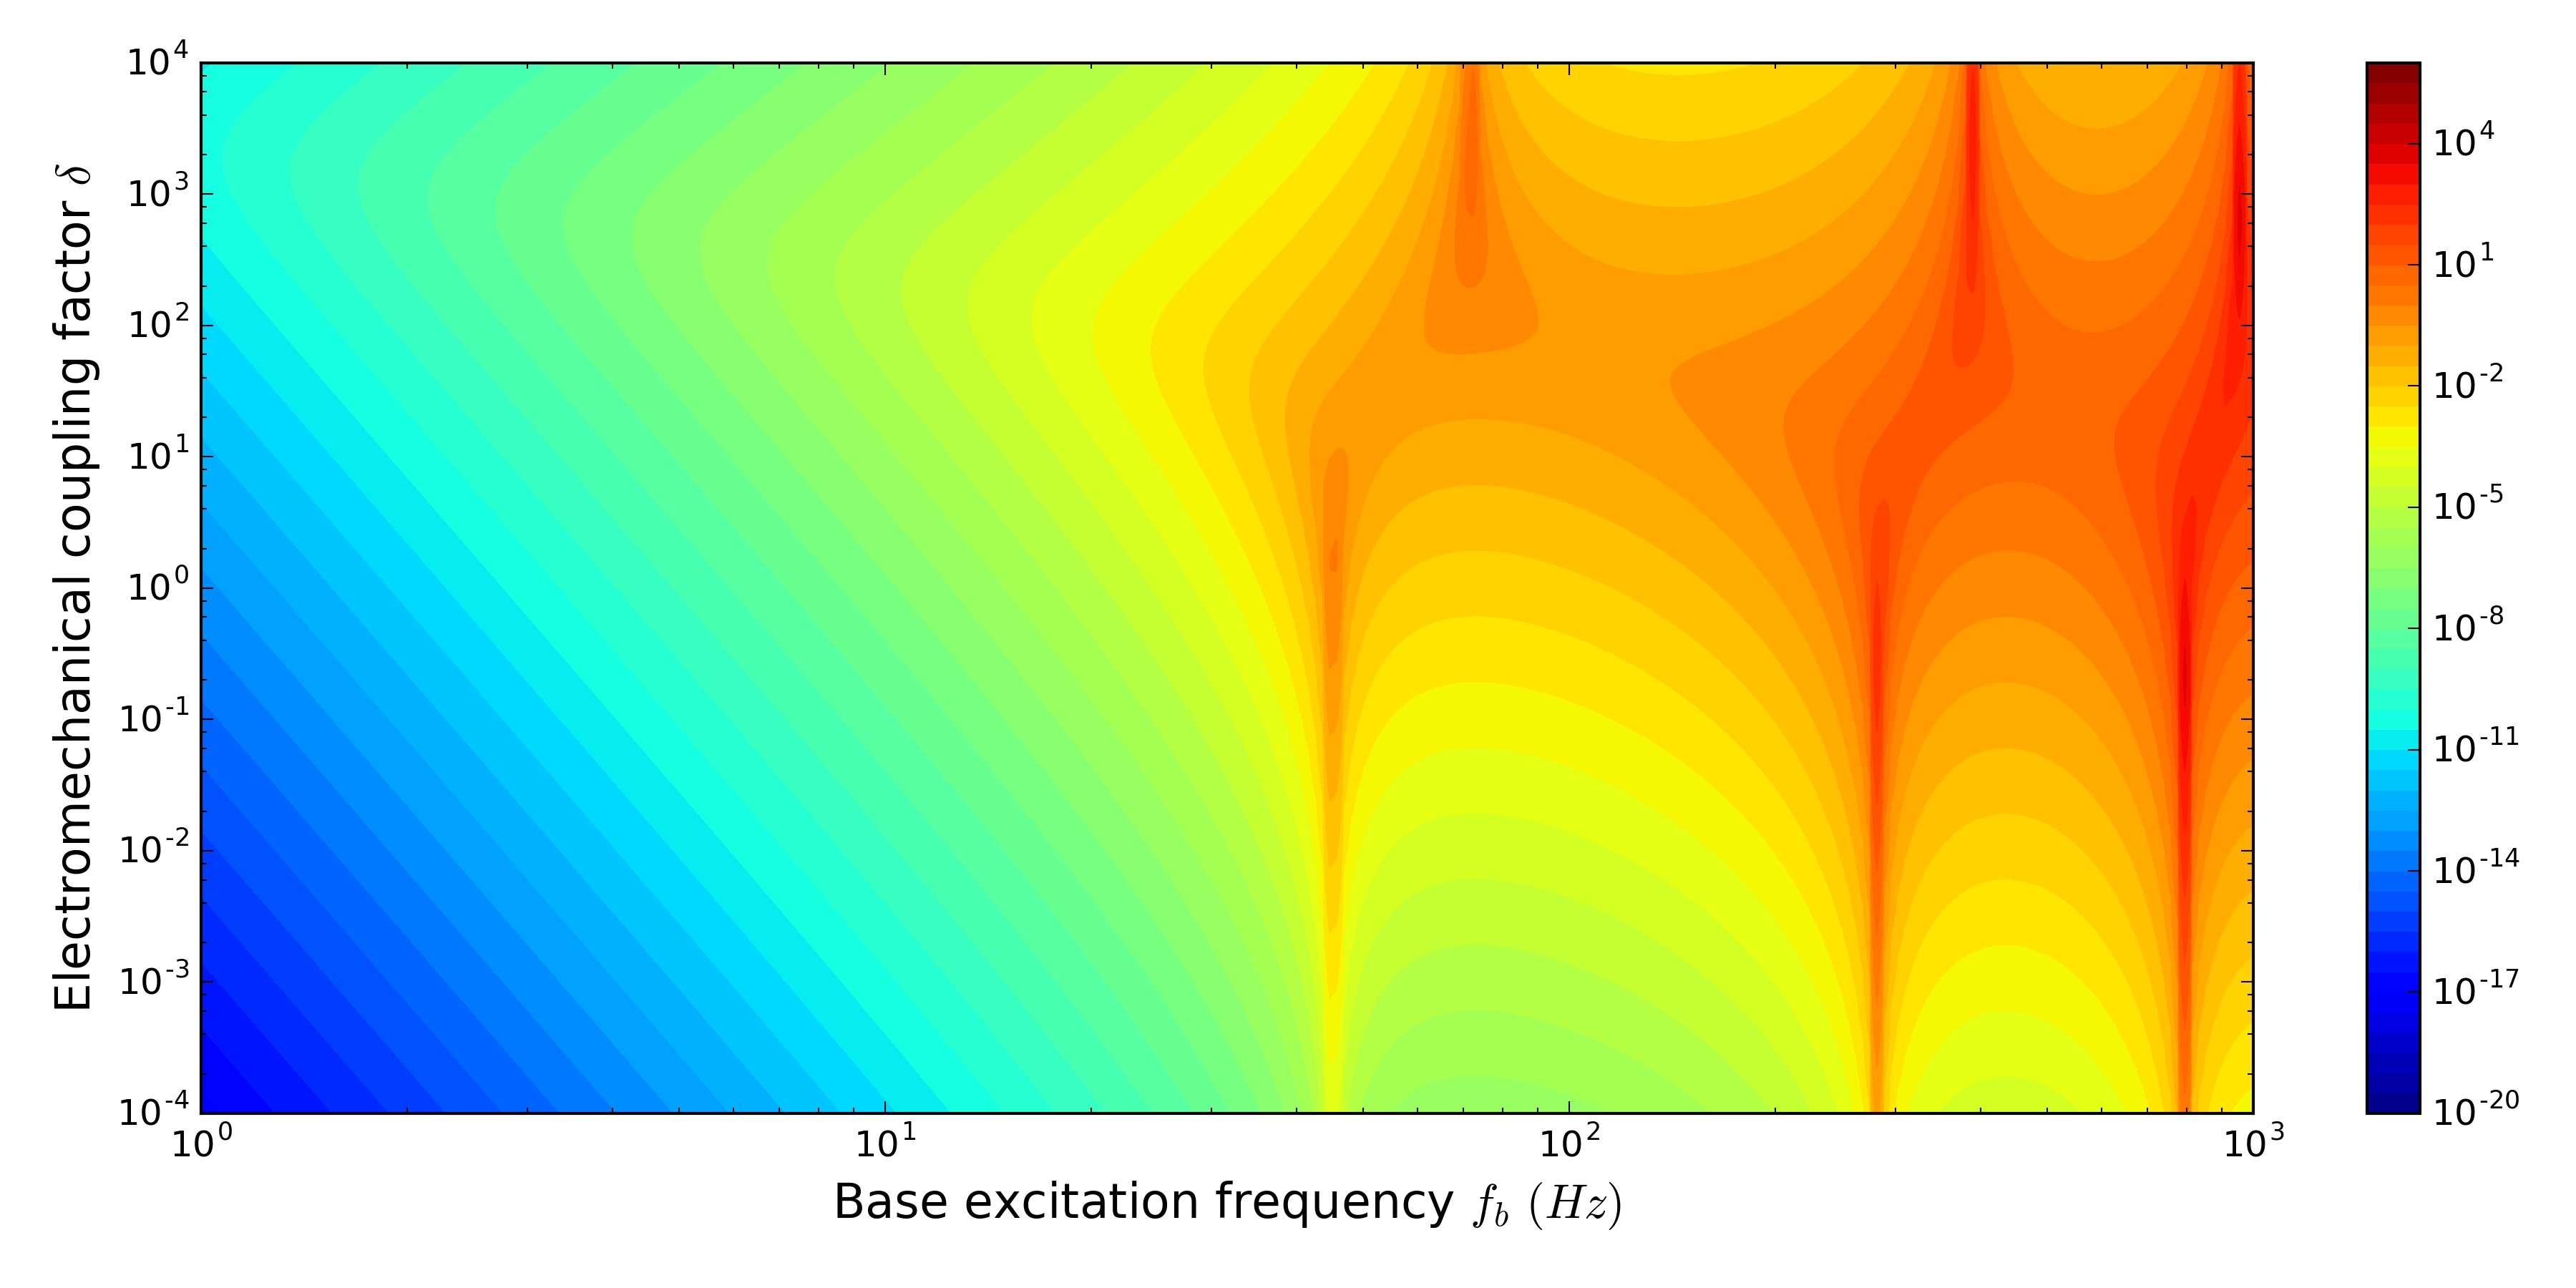
\includegraphics[width=\textwidth]{./img_eig_asy/fig_sol_analytic_out_vol_contour}
    \caption{Output voltage $\tilde{V}_p$ as a function of base excitation frequency $f_b$ and electromechanical coupling factor $\delta$.}
    \label{fig:fig_sol_analytic_out_vol_contour}
\end{figure}




\begin{figure}[!htbp]
    \centering
    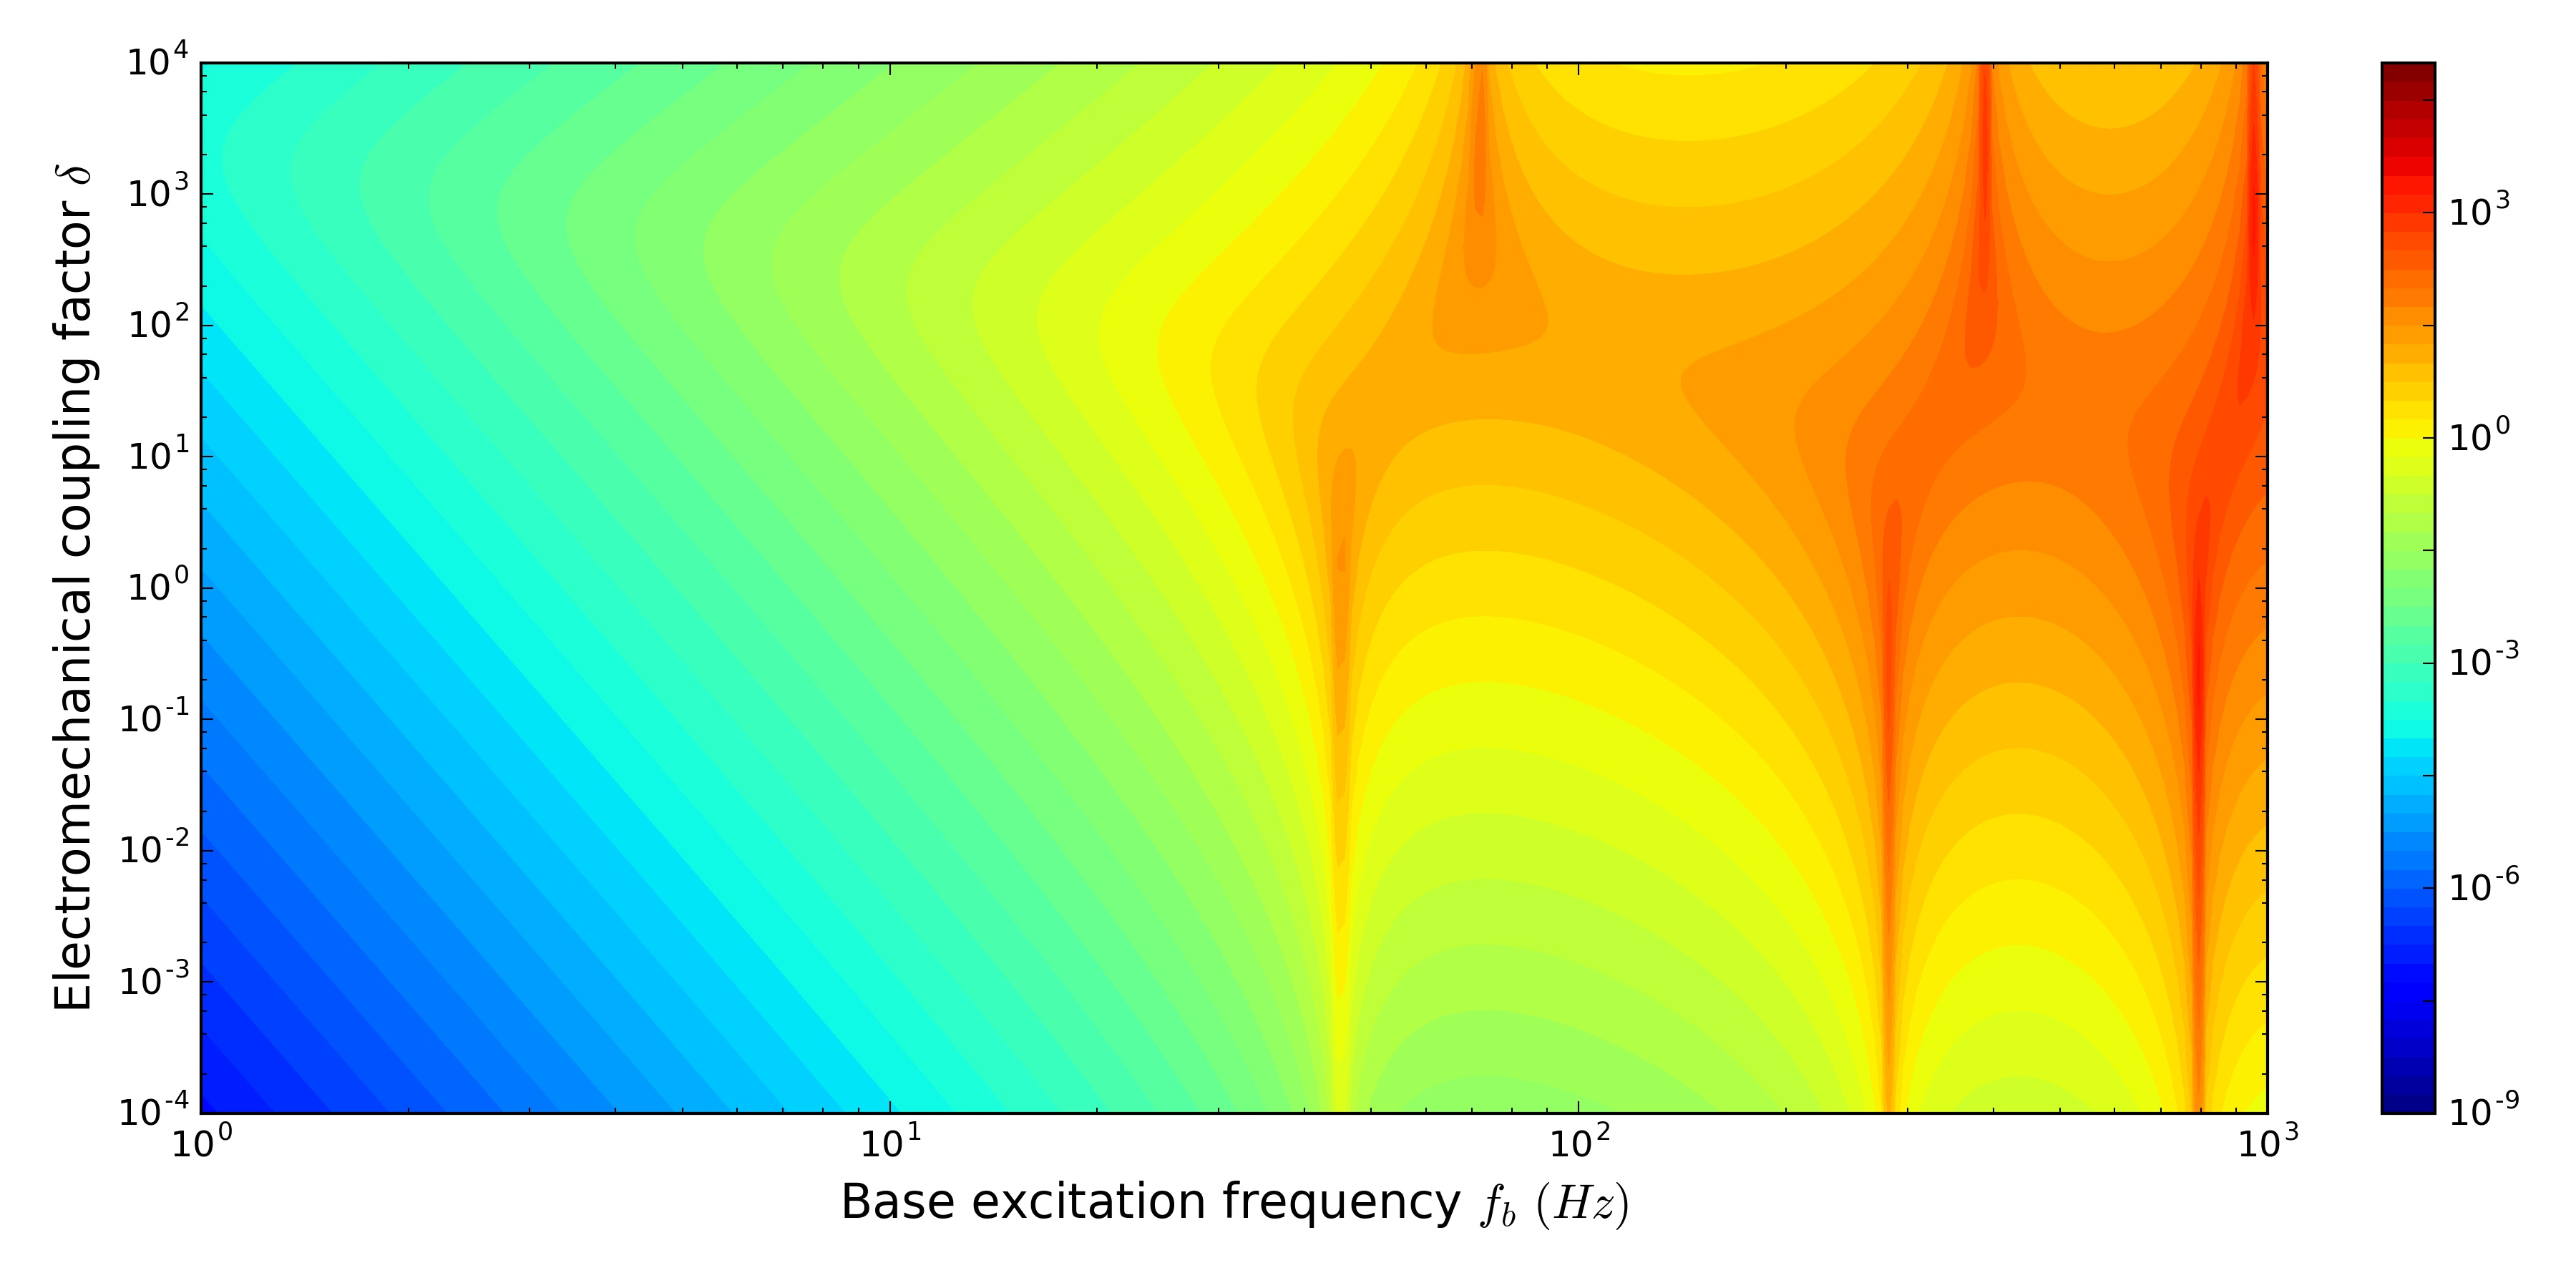
\includegraphics[width=\textwidth]{./img_eig_asy/fig_sol_analytic_out_pow_contour}
    \caption{Output voltage $\tilde{P}_p$ as a function of base excitation frequency $f_b$ and electromechanical coupling factor $\delta$.}
    \label{fig:fig_sol_analytic_out_pow_contour}
\end{figure}










\section{Conclusion}



















\section*{Appendices}

The asymptotic expansion of equation (\ref{eq:eq_disp_func_coeffs_exps}) can be found using an iterative method. In fact, for higher order expansions ($k \geq 1$), we have the following iterative relation: 
\begin{equation}
    \left\{\begin{aligned}
        A_{k+1} + C_{k+1} &= 0, \\
        B_{k+1} + D_{k+1} &= 0, \\
        \left( - A_{k+1} \cos{\sqrt{\sigma}} - B_{k+1} \sin{\sqrt{\sigma}} + C_{k+1} \cosh{\sqrt{\sigma}} + D_{k+1} \sinh{\sqrt{\sigma}} \right) &+ \\
        \frac{j \beta \sqrt{\sigma}}{ j\sigma \beta + 1 } \left( - A_{k} \sin{\sqrt{\sigma}} + B_{k} \cos{\sqrt{\sigma}} + C_{k} \sinh{\sqrt{\sigma}} + D_{k} \cosh{\sqrt{\sigma}} \right) &= 0, \\
        A_{k+1} \sin{\sqrt{\sigma}} - B_{k+1} \cos{\sqrt{\sigma}} + C_{k+1} \sinh{\sqrt{\sigma}} + D_{k+1} \cosh{\sqrt{\sigma}} &= 0,
    \end{aligned}\right.
\end{equation}
whose solution is expressed by
\begin{equation}
    \left\{\begin{aligned}
        A_{k+1} &= \left( \frac{j \beta \sqrt{\sigma }}{1+j \beta \sigma } \right) \left(\frac{\cos\sqrt{\sigma }+\cosh\sqrt{\sigma }}{2 \cos\sqrt{\sigma }\cosh\sqrt{\sigma }+2} \right) \left( Q_k \right), \\
        B_{k+1} &= \left( \frac{j \beta \sqrt{\sigma }}{1+j \beta \sigma } \right) \left( \frac{-\sinh\sqrt{\sigma }+\sin\sqrt{\sigma }}{2 \cos\sqrt{\sigma }\cosh\sqrt{\sigma }+2} \right) \left( Q_k \right), \\
        C_{k+1} &= \left( \frac{j \beta \sqrt{\sigma }}{1+j \beta \sigma } \right) \left( -\frac{\cos\sqrt{\sigma }+\cosh\sqrt{\sigma }}{2 \cos\sqrt{\sigma } \cosh\sqrt{\sigma }+2} \right) \left( Q_k \right), \\
        D_{k+1} &= \left( \frac{j \beta \sqrt{\sigma }}{1+j \beta \sigma } \right) \left( \frac{-\sin\sqrt{\sigma }+\sinh\sqrt{\sigma }}{2 \cos\sqrt{\sigma }\cosh\sqrt{\sigma }+2} \right) \left( Q_k \right), 
    \end{aligned}\right.
\end{equation}
in which
\begin{equation}
    Q_k = - A_{k} \sin{\sqrt{\sigma}} + B_{k} \cos{\sqrt{\sigma}} + C_{k} \sinh{\sqrt{\sigma}} + D_{k} \cosh{\sqrt{\sigma}}.
\end{equation}


In terms of $Q_k$ ($k \geq 0$), we have the following iterative relation
% \begin{equation}
%     \begin{aligned}
%         Q_{k+1} &= - A_{k+1} \sin{\sqrt{\sigma}} + B_{k+1} \cos{\sqrt{\sigma}} + C_{k+1} \sinh{\sqrt{\sigma}} + D_{k+1} \cosh{\sqrt{\sigma}} \\
%         &= - \left( \frac{ \sin\sqrt{\sigma} \cosh\sqrt{\sigma} + \cos\sqrt{\sigma} \sinh\sqrt{\sigma} }{ \cos\sqrt{\sigma }\cosh\sqrt{\sigma }+1 } \right) \left( \frac{j \beta \sqrt{\sigma }}{1+j \beta \sigma } \right) Q_k,
%     \end{aligned}
% \end{equation}
\begin{equation}
    Q_{k+1} = - \left( \frac{ \sin\sqrt{\sigma} \cosh\sqrt{\sigma} + \cos\sqrt{\sigma} \sinh\sqrt{\sigma} }{ \cos\sqrt{\sigma }\cosh\sqrt{\sigma }+1 } \right) \left( \frac{j \beta \sqrt{\sigma }}{1+j \beta \sigma } \right) Q_k,
\end{equation}
and the initial two values $Q_0$ and $Q_1$:
% \begin{equation}
%     \begin{aligned}
%         Q_{1} &= - A_1 \sin{\sqrt{\sigma}} + B_1 \cos{\sqrt{\sigma}} + C_1 \sinh{\sqrt{\sigma}} + D_1 \cosh{\sqrt{\sigma}} \\
%         &= \frac{j \beta  \sqrt{\sigma }}{1+j \beta  \sigma } \left(\frac{\sin\sqrt{\sigma } -\sinh\sqrt{\sigma }}{\cos\sqrt{\sigma } \cosh\sqrt{\sigma }+1} \right)  \left( \frac{\cos\sqrt{\sigma } \sinh\sqrt{\sigma }+\sin\sqrt{\sigma } \cosh\sqrt{\sigma }}{\cos\sqrt{\sigma } \cosh\sqrt{\sigma }+1} \right)
%     \end{aligned}
% \end{equation}
% \begin{equation}
%     Q_0 = \frac{\sinh\sqrt{\sigma }-\sin\sqrt{\sigma }}{\cos\sqrt{\sigma } \cosh\sqrt{\sigma }+1}
% \end{equation}
\begin{equation}
    \left\{\begin{aligned}
        Q_0 &= \frac{\sinh\sqrt{\sigma }-\sin\sqrt{\sigma }}{\cos\sqrt{\sigma } \cosh\sqrt{\sigma }+1}, \\
        Q_{1} &= \frac{j \beta  \sqrt{\sigma }}{1+j \beta  \sigma } \left(\frac{\sin\sqrt{\sigma } -\sinh\sqrt{\sigma }}{\cos\sqrt{\sigma } \cosh\sqrt{\sigma }+1} \right)  \left( \frac{\cos\sqrt{\sigma } \sinh\sqrt{\sigma }+\sin\sqrt{\sigma } \cosh\sqrt{\sigma }}{\cos\sqrt{\sigma } \cosh\sqrt{\sigma }+1} \right).
    \end{aligned}\right.
\end{equation}
Hence it is shown that for $k \geq 0$,
% \begin{equation}
%     \begin{aligned}
%         Q_{k} &= - \left( \frac{ \sin\sqrt{\sigma} \cosh\sqrt{\sigma} + \cos\sqrt{\sigma} \sinh\sqrt{\sigma} }{ \cos\sqrt{\sigma }\cosh\sqrt{\sigma }+1 } \right) \left( \frac{j \beta \sqrt{\sigma }}{1+j \beta \sigma } \right) Q_k \\
%         &= \left[- \left( \frac{j \beta \sqrt{\sigma }}{1+j \beta \sigma } \right) \left( \frac{ \sin\sqrt{\sigma} \cosh\sqrt{\sigma} + \cos\sqrt{\sigma} \sinh\sqrt{\sigma} }{ \cos\sqrt{\sigma }\cosh\sqrt{\sigma }+1 } \right)  \right]^k \left( \frac{\sinh\sqrt{\sigma }-\sin\sqrt{\sigma }}{\cos\sqrt{\sigma } \cosh\sqrt{\sigma }+1} \right)
%     \end{aligned}
% \end{equation}
\begin{equation}
    Q_{k} = \left[- \left( \frac{j \beta \sqrt{\sigma }}{1+j \beta \sigma } \right) \left( \frac{ \sin\sqrt{\sigma} \cosh\sqrt{\sigma} + \cos\sqrt{\sigma} \sinh\sqrt{\sigma} }{ \cos\sqrt{\sigma }\cosh\sqrt{\sigma }+1 } \right)  \right]^k \left( \frac{\sinh\sqrt{\sigma }-\sin\sqrt{\sigma }}{\cos\sqrt{\sigma } \cosh\sqrt{\sigma }+1} \right).
\end{equation}
As a result, we obtain that for $k \geq 1$,
\footnotesize
\begin{equation*}
    \left\{\begin{aligned}
        A_{k} &= \left( \frac{j \beta \sqrt{\sigma }}{1+j \beta \sigma } \right)^{k} \left( \frac{ -\sin\sqrt{\sigma} \cosh\sqrt{\sigma} - \cos\sqrt{\sigma} \sinh\sqrt{\sigma} }{ \cos\sqrt{\sigma }\cosh\sqrt{\sigma }+1 } \right)^{k-1} \left( \frac{\sinh\sqrt{\sigma }-\sin\sqrt{\sigma }}{\cos\sqrt{\sigma } \cosh\sqrt{\sigma }+1} \right) \left(\frac{\cos\sqrt{\sigma }+\cosh\sqrt{\sigma }}{2 \cos\sqrt{\sigma }\cosh\sqrt{\sigma }+2} \right), \\
        B_{k} &= \left( \frac{j \beta \sqrt{\sigma }}{1+j \beta \sigma } \right)^{k}  \left( \frac{ -\sin\sqrt{\sigma} \cosh\sqrt{\sigma} - \cos\sqrt{\sigma} \sinh\sqrt{\sigma} }{ \cos\sqrt{\sigma }\cosh\sqrt{\sigma }+1 } \right)^{k-1} \left( \frac{\sinh\sqrt{\sigma }-\sin\sqrt{\sigma }}{\cos\sqrt{\sigma } \cosh\sqrt{\sigma }+1} \right) \left( \frac{-\sinh\sqrt{\sigma }+\sin\sqrt{\sigma }}{2 \cos\sqrt{\sigma }\cosh\sqrt{\sigma }+2} \right), \\
        C_{k} &= \left( \frac{j \beta \sqrt{\sigma }}{1+j \beta \sigma } \right)^{k}  \left( \frac{ -\sin\sqrt{\sigma} \cosh\sqrt{\sigma} - \cos\sqrt{\sigma} \sinh\sqrt{\sigma} }{ \cos\sqrt{\sigma }\cosh\sqrt{\sigma }+1 } \right)^{k-1} \left( \frac{\sinh\sqrt{\sigma }-\sin\sqrt{\sigma }}{\cos\sqrt{\sigma } \cosh\sqrt{\sigma }+1} \right) \left( \frac{-\cos\sqrt{\sigma }-\cosh\sqrt{\sigma }}{2 \cos\sqrt{\sigma } \cosh\sqrt{\sigma }+2} \right), \\
        D_{k} &= \left( \frac{j \beta \sqrt{\sigma }}{1+j \beta \sigma } \right)^{k} \left( \frac{ -\sin\sqrt{\sigma} \cosh\sqrt{\sigma} - \cos\sqrt{\sigma} \sinh\sqrt{\sigma} }{ \cos\sqrt{\sigma }\cosh\sqrt{\sigma }+1 } \right)^{k-1} \left( \frac{\sinh\sqrt{\sigma }-\sin\sqrt{\sigma }}{\cos\sqrt{\sigma } \cosh\sqrt{\sigma }+1} \right) \left( \frac{-\sin\sqrt{\sigma }+\sinh\sqrt{\sigma }}{2 \cos\sqrt{\sigma }\cosh\sqrt{\sigma }+2} \right).
    \end{aligned}\right.
\end{equation*}
\normalsize



\section*{Acknowledgements}


\bibliography{analysis_eig_asy.bib}
\bibliographystyle{vancouver}

\end{document}